%%%%%%%%%%%%%%%%%%%%%%%%%%%%%%%%%%%%%%%%%%%%%%%%%%%%%%%%%%%%%%%%%%%%%%%%%%%%%%%%
\Chapter{
% 
    The Direct Current Feasibility Problem
% 
}{
% 
    An Algorithmic Approach to Computing Electrical Flows
% 
}{
% 
    \footnote{I would like to thank especially Matthias Wolf and Torsten
    Ueckerdt for questions, discussions, and comments. In addition, I
    would like to thank Marc Timme for some initial conversations, his time,
    and that he encouraged me (more or less) to write this chapter. }
% 
}
\label{ch:network-analysis}
\glsresetall
%%%%%%%%%%%%%%%%%%%%%%%%%%%%%%%%%%%%%%%%%%%%%%%%%%%%%%%%%%%%%%%%%%%%%%%%%%%%%%%% 
%
The~\acrlong{ac}~\acrlong{feas} (\gls{ac} \gls{feas};
see~\cref{ch:foundations:sec:power-flow-analyses:subsec:AC-Model})
and~\acrlong{dc}~\acrlong{feas} (\gls{dc} \gls{feas};
see~\cref{ch:foundations:sec:power-flow-analyses:subsec:Lin-DC-Model}) are
subproblems of most power grid related problems such as switching
(see~\cref{ch:switching}) and ideal~\gls{facts} placement (see~\cref{ch:facts}).
In this chapter, we formalize the operation of the power grid in such a way that
we are able to develop algorithmic approaches for the electrical flow
computation. With the latter formulations, we are able to develop better
algorithms for problems that incorporate the electrical flow computation as a
subproblem. Recall that one of the first persons who increased the knowledge
in~\gls{dc}~\gls{feas} was Kirchhoff~\parencite{Kir47}, who formalized the
electrical flow and introduced structural properties.

In~\cref{ch:foundations:sec:power-flow-analyses}, we described different models
and approximations to analyze the network by calculating the power flow, which
we call more generally electrical flow. In this chapter, we focus on
the~\acrlong{dc} \acrlong{feas} (\gls{dc}~\gls{feas}; commonly known
as~\acrlong{pf}; in short~\gls{pf}) and the~\gls{dc}~\acrlong{mpfp}
(\gls{dc}~\gls{mpfp}). We describe their mathematical models using different
formulations and give some structural insights that will be important to develop
algorithms for~\gls{dc}~\gls{feas} and~\gls{dc}~\gls{mpfp}
(see~\cref{ch:foundations:sec:power-flow-analyses:subsec:Lin-DC-Model}). Note
that one of the first algorithms---though with exponential running time---to
compute electrical flows uses spanning trees
(see~\cref{ch:network-analyzes:sec:mathematical-model:lem:current_edge_from_a_to_b};
\parencite{Ses61,Sha87}). We describe the latter
algorithm~\parencite{Ses61,Sha87} briefly
in~\cref{ch:network-analyzes:sec:mathematical-model}. This algorithm was used
by~\textcite{Fel13} to construct a squaring of a
rectangle~\parencite[pp.17ff.]{Fel13}. \citeauthor{Fel13} shows that the flow of
a graph that represents such a squaring of a rectangle is equivalent to a
solution of an integer~\gls{dc}~\gls{feas}, meaning all flows have to be
integral. Since this problem uses integral electrical flows (\ie, the flow is a
function~$
    % 
    \glssymbol{flow}
    \colon
    \glssymbol{edges}
    \to
    \integers
    % 
$), we usually cannot apply an~\gls{lp}
from~\cref{ch:foundations:sec:power-flow-analyses:subsec:Lin-DC-Model}, but have
to use an~\gls{ilp}. In general solving~\gls{ilp}s is~\NP-hard~\parencite[p.245;
MP1]{Gar79}. However, if the solution space has some properties, it is possible
to solve it with other techniques and algorithms in polynomial time. One
possibility would be to relax the variables of~\gls{dc}~\gls{feas}, which means
that a solution of an~\gls{lp} yields an integral solution. However, we show
that this technique does not necessarily result in an integral flow. However, if
we do not have a fixed generation, a fixed demand, and neglect the capacities,
meaning~$\glssymbol{capacity}\equiv\infty$, but ask for a generation and demand
such that we get integral electrical flows, we can make use of some properties
of the solution space. 
% This particular result shows us that there are integral
% electrical flows, which we will use for the runtime estimations.
% 
% However, we show that this is possible for that particular case,
% since the corners of the polytope (\ie, of the solution space) are on integral
% coordinates and get a~$\bigO(\fmagnitude{\glssymbol{vertices}}^{2.5})$
% algorithm~\parencite{Vai89,Bar75} for general graphs and
% an~$\bigO(\fmagnitude{\glssymbol{vertices}})$ algorithm for planar graphs.

In~\cref{ch:network-analyzes:sec:reduction-transformation-rules}, we first give
an overview over known transformation and contraction rules. In the end
of~\cref{ch:network-analyzes:sec:reduction-transformation-rules}, we give an
algorithm for the~\source-\sink-\gls{dc}~\gls{feas} and -\gls{mpfp} on planar
biconnected graphs that runs in~$\bigO(\fmagnitude{\glssymbol{vertices}}^3)$
time. Recall that~\gls{dc}~\gls{feas} and~\gls{mpfp} can be formulated as a
linear system of equations and an~\gls{lp}, respectively, that can be solved 
in~$\bigO(\fmagnitude{\glssymbol{edges}}^{2.5})$ time~\parencite{Vai89,Bar75}.
% 
Thus, using the contraction and transformation rules in the fashion described
in~\cref{ch:network-analyzes:sec:reduction-transformation-rules} does not yield
an algorithm that has a better running time than the known mathematical methods.
However, it gives some structural information.

While restricting our graphs to biconnected planar \source-\sink-graphs, we
develop an algorithm that transforms the formulation given
in~\cref{ch:foundations:sec:power-flow-analyses}
and~\cref{ch:network-analyzes:sec:mathematical-model} to an equivalent
formulation of~\emph{simultaneous flows}
(\cref{ch:network-analyzes:simultaneous-flow-representation}). For this
formulation, we are able to develop an algorithmic approach for~\source-\sink-
\gls{dc}~\gls{feas} and -\gls{mpf} algorithm for biconnected graphs
(\cref{ch:network-analyzes:sec:algorithm}) that can be extended to an algorithm
for multiple sources and multiple sinks on planar graphs by using the
superposition principle for linear physical systems.
% 
% 
%%%%%%%%%%%%%%%%%%%%%%%%%%%%%%%%%%%%%%%%%%%%%%%%%%%%%%%%%%%%%%%%%%%%%%%%%%%%%%%
\section[A Mathematical Model for the Feasibility Problem of Electrical Flows]{
A Mathematical Model for the \protect\linebreak{Feasibility Problem of Electrical Flows}} 
% 
\label{ch:network-analyzes:sec:mathematical-model}
%%%%%%%%%%%%%%%%%%%%%%%%%%%%%%%%%%%%%%%%%%%%%%%%%%%%%%%%%%%%%%%%%%%%%%%%%%%%%%%
% 
\textcite[p.13]{Cai12} give the structural hint that power grids are often
planar. Note that this might not be true in general. In addition, power grids
are quite sparse.
% 
The electrical network's topology is described by a bidirected
graph~$\glssymbol{graph} = (\glssymbol{vertices},\glssymbol{edges})$,
where~\glssymbol{vertices} is the set of vertices representing the buses (\ie,
line junctions), and~\glssymbol{edges} is the set of edges representing the
lines or cables (the conventional name is branch). Though the underlying graph
is undirected~\parencite[p.13]{Cai12}, we are always able to direct its
edges~$\{\vertexa,\vertexc\}\in
\glssymbol{undirectededges}$ by inserting two edges in opposite direction~$
(\vertexa,\vertexc), (\vertexc,\vertexa)\in\glssymbol{edges}$. Introducing the
direction is motivated by the electrical network's direction that is usually
defined by the voltage or current source representing the~\emph{reference}
vertex (also known as~\emph{slack} or~\emph{datum};
see~\cref{ch:foundations:tbl:load-flow-bus-specification} on
Page~\pageref{ch:foundations:tbl:load-flow-bus-specification}). The direction is
used for notational convenience and for electrical networks that
are~\emph{nonreciprocal}. Nonreciprocal electrical networks have components on
their edge that have a predefined direction such as diodes. However, in our case
the electrical network is reciprocal (also known as \emph{bilateral}) and thus,
the flow on each edge is allowed to flow in both directions. The underlying
graph is undirected, and we define for notational convenience the
set~\glssymbol{undirectededges} of undirected edges
by~$
    % 
    \glssymbol{undirectededges} 
    = 
    \{
        \undirectededge
        \mid
        \edge
        \in
        \glssymbol{edges}
    \}
    % 
$, \ie, $
% 
\makeUndirected{(\vertexa,\vertexc)} 
= 
\makeUndirected{(\vertexc,\vertexa)} 
= 
\{\vertexa,\vertexc\}
% 
$.

Each edge has a thermal limit and a susceptance that are represented by the
functions~$\glssymbol{capacity}\colon\glssymbol{undirectededges}\to\reals$
and~$\glssymbol{susceptance}\colon\glssymbol{undirectededges}\to\reals$,
respectively. The set~\glssymbol{generators} of generators represents the energy
sources and the demands are represented by a set~\glssymbol{consumers} of
consumers. Without loss of generality, we assume
that~$
    % 
    \glssymbol{generators}
    \cap
    \glssymbol{consumers}
    =
    \emptyset
    % 
$ and~$
    % 
    \glssymbol{generators}
    \cup
    \glssymbol{consumers}
    \subseteq
    \glssymbol{vertices}
    % 
$. An \emph{electrical network} is defined by a tuple~$\dcnetworktuple$ with
minimum and maximum generation~$
    % 
    \glssymbol{realpowergenerationmin},
    \glssymbol{realpowergenerationmax}
    \colon
    \glssymbol{vertices}
    \to
    \posreals
    \cup
    \{\infty\}
    % 
$, and minimum and maximum demand~$
    % 
    \glssymbol{realpowerdemandmin},
    \glssymbol{realpowerdemandmax}
    \colon
    \glssymbol{vertices}
    \to
    \posreals
    \cup\{\infty\}
    % 
$, respectively. In general, we distinguish between \emph{bounded} (\ie, $
    % 
    \vertexa
    \in
    \glssymbol{generators}
    \colon
    \glssymbol{realpowergenerationmax}(\vertexa)
    <
    \infty
    % 
$ and $
    % 
    \vertexa
    \in
    \glssymbol{consumers}
    \colon
    \glssymbol{realpowerdemandmax}(\vertexa)
    <
    \infty
    % 
$), \emph{unbounded} (\ie, $
    % 
    \glssymbol{realpowergenerationmax}
    \equiv
    \glssymbol{realpowerdemandmax}
    \equiv
    \infty
    % 
$), and \emph{exact} (\ie, $
    % 
    % \vertexa
    % \in
    % \glssymbol{generators}
    % \colon
    \glssymbol{realpowergenerationmin}%(\vertexa) 
    \equiv
    \glssymbol{realpowergenerationmax}%(\vertexa)
    % 
$ and~$
    % 
    % \vertexa
    % \in
    % \glssymbol{consumers}
    % \colon
    \glssymbol{realpowerdemandmin}%(\vertexa)
    \equiv
    \glssymbol{realpowerdemandmax}%(\vertexa)
    % 
$) networks.

The power is defined by current and voltage functions. These functions over time
map an edge and a point in time to voltage and current values
(see~\cref{ch:foundations:sec:power-flow-analyses:subsec:AC-Model}). However, in
this work we focus on \emph{steady-state} systems that are invariant and thus,
bind the functions to one particular timestamp. The latter means that all
functions become time independent.
%
A \emph{flow} is a function~$
    % 
    \glssymbol{flow}
    \colon
    \glssymbol{edges}
    \to
    \reals,
    (\vertexa,\vertexc)
    \mapsto
    \glssymbol{flow}(\vertexa,\vertexc)
    % 
$. A flow complies with the skew-symmetry
property~$
    % 
    \glssymbol{flow}(\vertexa,\vertexc) 
    = 
    -\glssymbol{flow}(\vertexc,\vertexa)
    % 
$ for all~$(\vertexa,\vertexc)\in\glssymbol{edges}$. The \emph{net flow} at a
vertex~$\vertexa\in\glssymbol{vertices}$ is defined by~$
    % 
    \glssymbol{netflow}(\vertexa)
    \coloneqq
    \sum_{
        \{\vertexa,\vertexc\}
        \in
        \glssymbol{undirectededges}
    }
    \glssymbol{flow}(\vertexa,\vertexc)
    % 
$. We define the \emph{flow value}~$
    % 
    \glssymbol{flowvalue}(\glssymbol{network},\glssymbol{flow})
    % 
$ to be the sum of all generator excesses~$
    % 
    \sum_{
        \vertexa
        \in
        \glssymbol{generators}
    }
    \glssymbol{netflow}(\vertexa)
    % 
$.

The behavior of voltage and current in the classical physics are described by
the Kirchhoff's laws~\parencite{Kir47}\parencite[p.120; Definition 6-1]{Ses61}.
Since we are interested in power flows while using a linearization of
an~\acrshort{ac} power flow (known as~\gls{dc}~\gls{feas}), we map~\gls{dc}
currents~$\current$ to real power~$
\glssymbol{realpower}$, which we denote by~$\glssymbol{flow}$
and~\gls{dc} voltage~$\voltage$ to voltage angle
differences~$\glssymbol{voltageangledifference}$ 
(see~\cref{ch:foundations:sec:power-flow-analyses:subsec:Lin-DC-Model} on
Page~\pageref{ch:foundations:sec:power-flow-analyses:analogies-to-the-dc-model}).
% 
%%%%%%%%%%%%%%%%%%%%%%%%%%%%%%%%%%%%%%%%%%%%%%%%%%%%%%%%%%%%%%%%%%%%%%%%%%%%%%%%
\paragraph{\acrlong{kcl} (\gls{kcl})}%
\label{ch:network-analyzes:sec:mathematical-model:kcl-flow}%
%%%%%%%%%%%%%%%%%%%%%%%%%%%%%%%%%%%%%%%%%%%%%%%%%%%%%%%%%%%%%%%%%%%%%%%%%%%%%%%%
% 
The first law is called the \emph{\acrlong{kcl}}~(\gls{kcl};
\crefrange{ch:network-analyzes:sec:mathematical-model:eq:KCL-intermediate-vertex}{ch:network-analyzes:sec:mathematical-model:eq:KCL-consumer-vertex})
and describes that the power entering a vertex~$\vertexa\in\glssymbol{vertices}$
is equal to the power exiting~\vertexa. This is equivalent to the conservation
of flow in graph theory.
%
\begin{align}%
% 
\glssymbol{netflow}(\vertexa) &= 0
&\forall\vertexa\in\glssymbol{vertices}\setminus
(\glssymbol{generators}\cup\glssymbol{consumers}),
\label{ch:network-analyzes:sec:mathematical-model:eq:KCL-intermediate-vertex}
\\%
% 
\glssymbol{realpowergenerationmin}(\vertexa)
\leq\glssymbol{netflow}(\vertexa)
&\leq\glssymbol{realpowergenerationmax}(\vertexa) 
&\forall\vertexa\in\glssymbol{generators},
\label{ch:network-analyzes:sec:mathematical-model:eq:KCL-generator-vertex}
\\%
% 
-\glssymbol{realpowerdemandmax}(\vertexa)
\leq\glssymbol{netflow}(\vertexa)
&\leq
-\glssymbol{realpowerdemandmin}(\vertexa)
&\forall\vertexa\in\glssymbol{consumers}.
\label{ch:network-analyzes:sec:mathematical-model:eq:KCL-consumer-vertex}%
% 
\end{align}%
%
The~\crefrange{ch:network-analyzes:sec:mathematical-model:eq:KCL-intermediate-vertex}{ch:network-analyzes:sec:mathematical-model:eq:KCL-consumer-vertex}
constrain the flow on the edges incident to a
vertex~$\vertexa\in\glssymbol{vertices}$. We distinguish between intermediate
vertices
(\cref{ch:network-analyzes:sec:mathematical-model:eq:KCL-intermediate-vertex}),
vertices with a generator
(\cref{ch:network-analyzes:sec:mathematical-model:eq:KCL-generator-vertex})
having an excess of power, and vertices with a consumer
(\cref{ch:network-analyzes:sec:mathematical-model:eq:KCL-consumer-vertex})
having a demand (disturbance) in power. Recall
from~\cref{ch:foundations:sec:power-flow-analyses:subsec:Lin-DC-Model} that the
latter equations
(\crefrange{ch:network-analyzes:sec:mathematical-model:eq:KCL-intermediate-vertex}{ch:network-analyzes:sec:mathematical-model:eq:KCL-consumer-vertex})
are equivalent
to~\crefrange{ch:foundations:sec:power-flow-analyses:dc:eq:kcl}{ch:foundations:sec:power-flow-analyses:dc:eq:angle-difference}.
Note that as long as we only consider the~\gls{kcl}, we can always connect
generator vertices~$\vertexa\in\glssymbol{generators}$ with a super
source~\source using~$\glssymbol{realpowergenerationmax}(\vertexa)$ as capacity,
and demand vertices~$\vertexa\in\glssymbol{consumers}$ with a super sink~\sink
using~$\glssymbol{realpowerdemandmax}(\vertexa)$ as capacity. This results in a
single-source and single-sink flow that is a notational simplification.
% 
% To model the lower generation and demand
% \franzi{matthias:? Either more detailed or don't mention it at all. Not here},
% we use the transformation shown by~\textcite[p.~343; Lemma~4.2]{Gra18}. 
% 
Note that we can connect the super source~\source and super sink~\sink
with each other resulting in a circulation problem. 

Though, the aforementioned formulation is our standard way to describe
the~\gls{kcl}, we need the algebraic formulation of the~\gls{kcl} to get some
structural insights. We assume from now on---if not stated otherwise---that we
have an exact network. Thus,
\cref{ch:network-analyzes:sec:mathematical-model:eq:KCL-generator-vertex,ch:network-analyzes:sec:mathematical-model:eq:KCL-consumer-vertex}
become~\cref{ch:network-analyzes:sec:mathematical-model:eq:kcl-matrix-writing:2,ch:network-analyzes:sec:mathematical-model:eq:kcl-matrix-writing:3}
with~$
    % 
    \glssymbol{realpowergeneration}
    \equiv
    \glssymbol{realpowergenerationmin}
    \equiv
    \glssymbol{realpowergenerationmax}
    % 
$ and~$
    % 
    \glssymbol{realpowerdemand}
    \equiv
    \glssymbol{realpowerdemandmin}
    \equiv
    \glssymbol{realpowerdemandmax}
    % 
$, respectively. Recall from~\cref{ch:foundations:sec:graph-theory} that an
oriented incidence matrix (also known as connection matrix) represents the
graph's connections in terms of the vertex-edge incidence relations, \ie, an
entry in row~\vertexa and column~\edge is~$1$ (respectively~$-1$) if edge~\edge
is an incoming (respectively outgoing) edge, and~$0$ otherwise. The properties
of such a matrix are given in~\cref{ch:foundations:sec:graph-theory}.
The~\crefrange{ch:network-analyzes:sec:mathematical-model:eq:KCL-intermediate-vertex}{ch:network-analyzes:sec:mathematical-model:eq:KCL-consumer-vertex}
can be restated using the oriented incidence
matrix~$
    % 
    \glssymbol{incidenceMatrix}
    \in
    \{-1,0,1\}^{
        \fmagnitude{
            \glssymbol{vertices}
        }
        \times
        \fmagnitude{
            \glssymbol{edges}
        }
    }
    % 
$ and the vector of flows~$
    \vv{
        \glssymbol{flow}
    }
    \in
    \reals^{
        \fmagnitude{
            \glssymbol{edges}
        }
    }
    % 
$ with~$
    % 
    \vv{
        \glssymbol{flow}
    } 
    \coloneqq
    \big(
        \glssymbol{flow}(\vertexa,\vertexc)
    \big)_{ 
        (\vertexa,\vertexc)
        \in
        \glssymbol{edges}
    % 
}$. The~\gls{kcl} in matrix form is given
in~\crefrange{ch:network-analyzes:sec:mathematical-model:eq:kcl-matrix-writing:1}{ch:network-analyzes:sec:mathematical-model:eq:kcl-matrix-writing:3}.
%
\begin{align}
    % 
    \glssymbol{incidenceMatrix}_{
        \glssymbol{vertices}
        \setminus
        (
            \glssymbol{generators}
            \cup
            \glssymbol{consumers}
        )
    } 
    \vv{
        \glssymbol{flow}
    } 
    &= 
    \vv{0},
    % 
    \label{ch:network-analyzes:sec:mathematical-model:eq:kcl-matrix-writing:1}
    % 
    \\
    % 
    \glssymbol{incidenceMatrix}_{
        \glssymbol{generators}
    } 
    \vv{
        \glssymbol{flow}
    }
    &= 
    \vv{
        \glssymbol{realpowergeneration}
    },
    % 
    \label{ch:network-analyzes:sec:mathematical-model:eq:kcl-matrix-writing:2}
    \\
    % 
    \glssymbol{incidenceMatrix}_{
        \glssymbol{consumers}
    }
    \vv{
        \glssymbol{flow}
    } 
    &=
    \vv{\glssymbol{realpowerdemand}},
    % 
    \label{ch:network-analyzes:sec:mathematical-model:eq:kcl-matrix-writing:3}
    % 
\end{align}
%
where~$\vv{0}$ is the zero vector of size~$
% 
\fmagnitude{
    \glssymbol{vertices}
    \setminus
    (
        \glssymbol{generators}
        \cup
        \glssymbol{consumers}
    )
}
% 
$,
$
% 
\glssymbol{incidenceMatrix}_{
    \glssymbol{vertices}
    \setminus
    (
        \glssymbol{generators}
        \cup
        \glssymbol{consumers}
    )
}
% 
$ is a submatrix of the incidence matrix~\glssymbol{incidenceMatrix} constituted
by the vertices that are neither generators nor consumers. Similar notion is
used for the submatrix of the generators and consumers
in~\cref{ch:network-analyzes:sec:mathematical-model:eq:kcl-matrix-writing:2}
and~\cref{ch:network-analyzes:sec:mathematical-model:eq:kcl-matrix-writing:3}.
Note when~$
    % 
    (\source,\sink)
    \in
    \glssymbol{edges}
    % 
$ the flow vector~$\vv{\glssymbol{flow}}$ would have a fixed entry with~$
    % 
    \vv{
        \glssymbol{flow}
    }_{(\source,\sink)} 
    =
    \sum_{\vertexa\in\generators}
    \glssymbol{realpowergeneration}(\vertexa) 
    =
    \sum_{\vertexc\in\consumers}
    \glssymbol{realpowerdemand}(\vertexc)
    % 
$ 
and~\cref{ch:network-analyzes:sec:mathematical-model:eq:kcl-matrix-writing:1} is
sufficient.
\crefrange{ch:network-analyzes:sec:mathematical-model:eq:kcl-matrix-writing:1}
{ch:network-analyzes:sec:mathematical-model:eq:kcl-matrix-writing:3} constitute
an incidence matrix~$
    % 
    \glssymbol{incidenceMatrix}
    \in
    \reals^{
        \fmagnitude{\glssymbol{vertices}
    } 
    \times 
    \fmagnitude{
        \glssymbol{edges}
    } 
    % 
}$ with~$
    % 
    \glssymbol{incidenceMatrix}
    \coloneqq 
    \transpose{
        (
            \glssymbol{incidenceMatrix}_{
                \glssymbol{vertices}
                \setminus
                (
                    \glssymbol{generators}
                    \cup
                    \glssymbol{consumers}
                )
            },   
            \glssymbol{incidenceMatrix}_{
                \glssymbol{generators}
            },
            \glssymbol{incidenceMatrix}_{
                \glssymbol{consumers}
            }
        )
    }
    % 
$ and right-hand side vector~$
    % 
    \frighthandsidevector{ \glssymbol{incidenceMatrix} }
    \in
    \reals^{ \fmagnitude{\glssymbol{vertices}} }
    % 
$ with~$
    \frighthandsidevector{ \glssymbol{incidenceMatrix} }
    \coloneqq
    \transpose{
        (
            \vv{0},
            \vv{\glssymbol{realpowergeneration}},
            \vv{\glssymbol{realpowerdemand}}
        )
    }
$. 
% 
The whole system of linear equations is given
in~\cref{ch:network-analyzes:sec:mathematical-model:eq:kcl-matrix-writing}.
% 
\begin{equation}
    \glssymbol{incidenceMatrix} 
    \cdot 
    \vv{\glssymbol{flow}} 
    = 
    \frighthandsidevector{ \glssymbol{incidenceMatrix} }. 
    % 
    \label{ch:network-analyzes:sec:mathematical-model:eq:kcl-matrix-writing}
    % 
\end{equation}
% 
The system~$
% 
\glssymbol{incidenceMatrix}
\cdot
\vv{ \glssymbol{flow} }
=
\frighthandsidevector{ \glssymbol{incidenceMatrix} }
% =
% \transpose{(\vv{0},\vv{\realpowergeneration},\vv{\realpowerdemand})}
% 
$ represents a translation of the solution set~$
    % 
    \glssymbol{incidenceMatrix}
    \cdot
    \vv{ \glssymbol{flow} }
    =
    \vv{0}
    %
$. 
% 
The latter equation is also called \emph{homogeneous equation} (or homogeneous
problem) and has always the trivial solution~$
    % 
    \vv{\glssymbol{flow}} 
    = 
    \vv{0}
    % 
$. 
% Note that the rows of the incidence matrix~$
%      % 
%     \glssymbol{incidenceMatrix}_{
%             \glssymbol{vertices}
%             \setminus
%             (
%                 \glssymbol{generators}
%                 \cup
%                 \glssymbol{consumers}
%             )
%         } 
%     % 
% $ are linearly independent if the homogeneous equation has only the trivial
% solution. 
% 
If we have a solution~$\vv{\glssymbol{flow}}_{\mathrm{nh}}$ for the
nonhomogeneous system then the whole solution space can be described
by~$
    \vv{\glssymbol{flow}}_{\mathrm{nh}} 
    +  
    \{ 
        \vv{\glssymbol{flow}}_{\mathrm{h}}
    \mid
        \vv{\glssymbol{flow}}_{\mathrm{h}}
        \in
        \reals^{\fmagnitude{\gls{edges}}},
        \glssymbol{incidenceMatrix}
        \cdot
        \vv{\glssymbol{flow}}_{\mathrm{h}}
        =
        \vv{0}
    \}
    % 
$,
where~$\vv{\glssymbol{flow}}_{\mathrm{h}}$ is a solution vector of the
homogeneous system.
%
%%%%%%%%%%%%%%%%%%%%%%%%%%%%%%%%%%%%%%%%%%%%%%%%%%%%%%%%%%%%%%%%%%%%%%%%%%%%%%%% 
\paragraph{\gls{kcl} Flow}
\label{ch:network-analyzes:sec:mathematical-model:paragraph:kcl-flow}
%%%%%%%%%%%%%%%%%%%%%%%%%%%%%%%%%%%%%%%%%%%%%%%%%%%%%%%%%%%%%%%%%%%%%%%%%%%%%%%%
% 
We call a flow~\glssymbol{flow} complying with the~\gls{kcl} as
a~\emph{\gls{kcl} flow}. Recall that we can interpret vectors in the euclidean
space geometrically as a line segment from the origin with magnitude and
direction. Two vectors are orthogonal to each other if the angle~$\alpha$
between them is~$90^\circ$ and~$\cos (\nicefrac{\glssymbol{pi}}{2}) = 0$. Thus,
the dot product is zero meaning~$
    % 
    % \glssymbol{incidenceMatrix}
    \incidenceMatrixElement{\vertexa}
    \cdot
    \vv{\glssymbol{flow}} 
    = 
    \vv{0}
    % 
$, since~$
    % 
    \incidenceMatrixElement{\vertexa}
    \vv{\glssymbol{flow}} 
    =
    \norm{
        \incidenceMatrixElement{\vertexa}
    }{2}
    % 
    \norm{
        \vv{\glssymbol{flow}}
    }{2}
    \cos(\alpha)
    % 
$ for all vertices~$\vertexa\in\glssymbol{vertices}$. If we have~$
    % 
    \glssymbol{incidenceMatrix}
    \cdot
    \vv{\glssymbol{flow}} 
    = 
    \vv{0}
    % 
$ this implies that every vector~$\incidenceMatrixElement{\vertexa}$ in the
vector space (here a row~\vertexa in~$\glssymbol{incidenceMatrix}$) is
orthogonal to the vector~$\vv{\glssymbol{flow}}$.
% 
%%%%%%%%%%%%%%%%%%%%%%%%%%%%%%%%%%%%%%%%%%%%%%%%%%%%%%%%%%%%%%%%%%%%%%%%%%%%%%%%
\paragraph{Properties of the Incidence Matrix}
\label{ch:network-analyzes:sec:mathematical-model:paragraph:property-incidence-matrix}
%%%%%%%%%%%%%%%%%%%%%%%%%%%%%%%%%%%%%%%%%%%%%%%%%%%%%%%%%%%%%%%%%%%%%%%%%%%%%%%%
% 
Note
that~\cref{ch:network-analyzes:sec:mathematical-model:eq:kcl-matrix-writing:1}
means that the incidence matrix~\glssymbol{incidenceMatrix} and the vector~$
\vv{\glssymbol{flow}}$ are orthogonal to each other---meaning every row vector
of~\glssymbol{incidenceMatrix} is orthogonal to~$\vv{\glssymbol{flow}}$. Note
that this implies that the vectors are also linear independent, since there is
no scalar that makes~$\vv{
\glssymbol{flow}}$ colinear to one of the vertices
in~\glssymbol{incidenceMatrix}. The latter is equivalent to~$
% 
\vv{\glssymbol{flow}}
\in
\fkernel{\glssymbol{incidenceMatrix}}
% 
$ with~$
% 
\fkernel{\glssymbol{incidenceMatrix}}
\coloneqq
\{
    \vv{
        \glssymbol{flow}
    } 
    \in 
    \reals^{ \fmagnitude{ \glssymbol{edges} } }
    \mid
    \glssymbol{incidenceMatrix}
    \cdot
    \vv{\glssymbol{flow}} 
    = 
    \vv{0}
\}
\subseteq
\reals^{\fmagnitude{\glssymbol{edges}}}
% 
$. 

% 
\begin{wrapfigure}{l}{4.5cm}%
    % 
    \vspace{-4mm}
    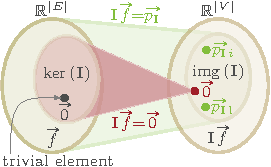
\includegraphics[scale=1,page=1]{networkAnalyzes/figures/ImageAndKernelOfALinearMappingIncidenceMatrix.pdf}
    % 
    \vspace{-5mm}%
    \caption[The image and kernel of the incidence
    matrix~\glssymbol{incidenceMatrix}.]{%
    % 
    The image~$\fimage{\glssymbol{incidenceMatrix}}$ and kernel~$\fkernel{
    \glssymbol{incidenceMatrix}}$ of the incidence
    matrix~\glssymbol{incidenceMatrix} for the linear map~$
        % 
        \glssymbol{incidenceMatrix}
        \colon
        \reals^{
            \fmagnitude{\glssymbol{edges}}
        }
        \to
        \reals^{
            \fmagnitude{\glssymbol{vertices}}
        }
        % 
    $.
    %
    }%
    % 
    \label{ch:network-analysis:fig:kernel-and-image-incidenceMatrix}%
    \vspace{-2mm}%
    % 
\end{wrapfigure}%
% 
\noindent Note that a \emph{trivial element} of the kernel is the neutral
element, \ie, in the vector space this is the zero vector~$\vv{0}$
(see~\cref{ch:network-analysis:fig:kernel-and-image-incidenceMatrix} left side).
If the kernel consists of the neutral element only then the linear map is
injective.
% 
% The dimension or size of the kernel, thus, describes the degree by which we
% fail the injectivity.
% 
From~\textcite[p.66; Theorem 4--3]{Ses61}, we know that the rank of the
matrix~\glssymbol{incidenceMatrix} is~$
% 
\rankx{ \glssymbol{incidenceMatrix} }
=
\fmagnitude{ \glssymbol{vertices} } 
- 
k
% 
$ with~$k$ being the number of connected components.
% 
The idea is that summing up the rows leads to one row of zeros per connected
component, since every column of the incidence
matrix~\glssymbol{incidenceMatrix}---representing an edge---consists of exactly
one~$1$ entry and one~$-1$ entry, which gives us~$
    % 
    \rankx{\glssymbol{incidenceMatrix}} 
    \leq 
    \fmagnitude{ \glssymbol{vertices} }
    - k
    % 
$
(see~\cref{ch:network-analyzes:sec:mathematical-model:fig:TUM-proof}\screen{b}
on Page~\pageref{ch:network-analyzes:sec:mathematical-model:fig:TUM-proof} as 
example). The aforementioned structure of the incidence
matrix~\glssymbol{incidenceMatrix} leads to an upper triangle matrix for each
connected component that cannot be reduced further leading to~$
    % 
    \rankx{\glssymbol{incidenceMatrix}} 
    \geq 
    \fmagnitude{ \glssymbol{vertices} } 
    - k
    % 
$ and thus, $
    % 
    \rankx{\glssymbol{incidenceMatrix}} 
    = 
    \fmagnitude{ \glssymbol{vertices} } 
    - k
    % 
$.
% 
Recall that the rank of the incidence matrix~\glssymbol{incidenceMatrix} (\ie,
$\rankx{\glssymbol{incidenceMatrix}}$) corresponds to the number of edges in a
spanning forest. To determine the nullity~$
    % 
    \nullityx{\glssymbol{incidenceMatrix}} 
    \coloneqq 
    \dimensionx{\fkernel{\glssymbol{incidenceMatrix}}}
    % 
$ of the incidence matrix~\glssymbol{incidenceMatrix}, we introduce
the~\emph{rank-nullity theorem}.
% 
\begin{theorem}[Rank-nullity Theorem]
    For any matrix~$\constraintmatrix\in\reals^{r\times c}$ with~$r$ rows
    and~$c$ columns the rank~$\rank(\constraintmatrix)$ and
    nullity~$\nullity(\constraintmatrix)$ sum up to the number of columns.
    % 
    $$
        \rankx{\constraintmatrix} 
        + 
        \nullityx{\constraintmatrix} 
        = 
        c.
    $$
    % 
    The generalization to linear maps~$
        % 
        \constraintmatrix
        \colon 
        \reals^{ \fmagnitude{C} } 
        \to
        \reals^{ \fmagnitude{R} }
        % 
    $ is given by
    % 
    $$
        \dimensionx{\fimage{\constraintmatrix}} 
        + 
        \dimensionx{\fkernel{\constraintmatrix}} 
        =
        \dimensionx{ \reals^{ \fmagnitude{C} } }
        =
        \fmagnitude{C}.
    $$
    % 
    \label{ch:network-analysis:def:rank-nullity-theorem}
    % 
\end{theorem}
%
The incidence matrix~\glssymbol{incidenceMatrix} can be viewed as a linear map~$
    % 
    \glssymbol{incidenceMatrix}
    \colon
    \reals^{
        \fmagnitude{
            \glssymbol{edges}
        }
    }
    \to
    \reals^{
        \fmagnitude{
            \glssymbol{vertices}
        }
    }
    % 
$ with $
    % 
    \vv{\glssymbol{flow}}
    \mapsto
    \glssymbol{incidenceMatrix}
    \cdot
    \vv{\glssymbol{flow}}
    % 
$. The kernel~$\fkernel{\glssymbol{incidenceMatrix}}$ and
image~$\fimage{\glssymbol{incidenceMatrix}}$ of the incidence
matrix~\glssymbol{incidenceMatrix} are given
in~\cref{ch:network-analysis:eq:incidence-matrix-image-and-kernel}.
% 
\begin{subequations}% 
\begin{align}%
    % 
    \fkernel{\glssymbol{incidenceMatrix}}
    &
    \coloneqq 
    \{
        \vv{\glssymbol{flow}}
        \in
        \reals^{\fmagnitude{\glssymbol{edges}}}
        \mid 
        \glssymbol{incidenceMatrix}
        \cdot
        \vv{\glssymbol{flow}} 
        = 
        \vv{0}
    \} 
    &
    \subseteq
    \reals^{\fmagnitude{\glssymbol{edges}}}
    % 
    \label{ch:network-analysis:eq:incidence-matrix-kernel}
    % 
    \\
    % 
    \fimage{\glssymbol{incidenceMatrix}}
    &
    \coloneqq 
    \{
        \frighthandsidevector{\glssymbol{incidenceMatrix}}
        \in
        \reals^{\fmagnitude{\glssymbol{vertices}}}
        \mid 
        \exists
        \vv{\glssymbol{flow}}
        \in
        \reals^{\fmagnitude{\glssymbol{edges}}}
        \colon 
        \glssymbol{incidenceMatrix}
        \cdot
        \vv{\glssymbol{flow}} 
        = 
        \frighthandsidevector{\glssymbol{incidenceMatrix}}
    \} 
    &
    \subseteq
    \reals^{\fmagnitude{\glssymbol{vertices}}}
    % 
    \label{ch:network-analysis:eq:incidence-matrix-image}
    % 
\end{align}%
\label{ch:network-analysis:eq:incidence-matrix-image-and-kernel}
% 
\end{subequations}% 
%
A kernel~$\fkernel{\glssymbol{incidenceMatrix}}$ of the incidence
matrix~\glssymbol{incidenceMatrix} is a set~$\fkernel{
\glssymbol{incidenceMatrix}}$ of vectors~$\vv{\glssymbol{flow}}$ such that the
homogeneous system~$
    % 
    \glssymbol{incidenceMatrix}
    \cdot
    \vv{ \glssymbol{flow} }
    = 
    \vv{0}
    % 
$ holds for all vectors in that set 
(see~\cref{ch:network-analysis:fig:kernel-and-image-incidenceMatrix} red area
and text). The image~$\fimage{\glssymbol{incidenceMatrix}}$ of the incidence
matrix are all vectors~$\frighthandsidevector{\glssymbol{incidenceMatrix}}$ for
which a solution exist 
(see~\cref{ch:network-analysis:fig:kernel-and-image-incidenceMatrix} green area
and text).
 
Using the rank-nullity theorem 
(see~\cref{ch:network-analysis:def:rank-nullity-theorem}) we get the dimension
of the kernel (\ie, the nullity when talking about matrices)
of~$
    % 
    \dimensionx{\fkernel{\glssymbol{incidenceMatrix}}}
    =
    \dimensionx{\glssymbol{edges}}
    -
    \dimensionx{\fimage{\glssymbol{incidenceMatrix}}}
    =
    \fmagnitude{\glssymbol{edges}} 
    - 
    \fmagnitude{\glssymbol{vertices}} 
    + k
    % 
$ 
%
that corresponds to the number of chords (\ie, edges not on a spanning forest).
A common way to construct the incidence matrix~\glssymbol{incidenceMatrix}
(see~\cref{ch:foundations} on Page~\pageref{ch:foundations:incidence-matrix}) of
row size~$\fmagnitude{\glssymbol{vertices}} - k$ is to define one
vertex~$\vertexa\in\glssymbol{generators}$ per connected component as slack%

% 
\begin{wrapfigure}{l}{3.5cm}%
    % 
    % \vspace{-4mm}
    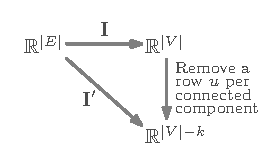
\includegraphics[scale=1,page=1]{networkAnalyzes/figures/NotesOnTheIncidenceProperty.pdf}
    % 
    % \vspace{-4mm}%
    \caption[Linear maps of the incidence matrix~\glssymbol{incidenceMatrix}.]{%
    Linear maps of the incidence matrix~\glssymbol{incidenceMatrix}
    and~$\glssymbol{incidenceMatrix}'$, where~$k$ is the number of connected
    components.
    %
    }%
    % 
    \label{ch:network-analysis:fig:mapping-incidenceMatrix}%
    % \vspace{-2mm}%
    % 
\end{wrapfigure}%
%
\noindent vertex and remove its row~$\vertexa$ (see
example~\cref{ch:network-analyzes:sec:mathematical-model:fig:TUM-proof}
\screen{b} on Page~\pageref{ch:network-analyzes:sec:mathematical-model:fig:TUM-proof},
where we remove vertex~$3$). From the property of the incidence
matrix~\glssymbol{incidenceMatrix} we know that every square submatrix
of~\glssymbol{incidenceMatrix} has a determinant that is either~$-1$, $0$,
or~$1$. Since every square non-singular submatrix of the incidence
matrix~\glssymbol{incidenceMatrix} of
size~$(\fmagnitude{\glssymbol{vertices}}-k)\times(\fmagnitude{
\glssymbol{vertices}}-k)$ that is the maximum square submatrix that constitutes
a spanning tree is unimodular (\ie, the determinant takes~$\pm 1$ values only)
and all determinants are either~$0, 1$, or~$-1$, the incidence
matrix~\glssymbol{incidenceMatrix} is \acrlong{tum} (in short~\gls{tum}).

\noindent If not noted otherwise, if we speak from now on of the incidence
matrix~\glssymbol{incidenceMatrix}, we mean the reduced incidence matrix that
has~$\fmagnitude{\glssymbol{vertices}}-k$ rows and thus, is defined by~$
    % 
    \glssymbol{incidenceMatrix}
    \in
    \{-1,0,1\}^{
        (
            \fmagnitude{\glssymbol{vertices}}-k
        )
        \times
        \fmagnitude{\glssymbol{edges}}
    }
    % 
$ (see~\cref{ch:network-analysis:fig:mapping-incidenceMatrix}).
% 
% 
%%%%%%%%%%%%%%%%%%%%%%%%%%%%%%%%%%%%%%%%%%%%%%%%%%%%%%%%%%%%%%%%%%%%%%%%%%%%%%%%
\paragraph{Feasible Flows and Thermal Line Limit}
\label{ch:network-analyzes:sec:mathematical-model:paragraph:capacity}
%%%%%%%%%%%%%%%%%%%%%%%%%%%%%%%%%%%%%%%%%%%%%%%%%%%%%%%%%%%%%%%%%%%%%%%%%%%%%%%%
% 
As already mentioned each edge has a natural limit of flow it is able to carry.
This is usually modeled by the capacity constraint that basically models the
thermal line limit
(\cref{ch:network-analyzes:sec:mathematical-model:eq:capacity-constraint}).
%
\begin{align}
    % 
    \fmagnitude{\glssymbol{flow}(\vertexa,\vertexc)}
    \leq
    \glssymbol{capacity}(\vertexa,\vertexc)
    \qquad
    \forall(\vertexa,\vertexc)\in\glssymbol{edges}.
    % 
    \label{ch:network-analyzes:sec:mathematical-model:eq:capacity-constraint}
\end{align}
%
We denote a flow~\glssymbol{flow} complying with the capacity constraints
as~\emph{feasible flow}. A~\gls{kcl} flow (see~\gls{kcl} flow on
Page~\pageref{ch:network-analyzes:sec:mathematical-model:paragraph:kcl-flow})
complying with the capacity constraint is thus called a~\emph{feasible~\gls{kcl}
flow}.
% 
\paragraph{\acrlong{kvl} (\gls{kvl})}
\label{ch:network-analyzes:sec:mathematical-model:paragraph:kvl}
% 
Kirchhoff's second law is known as~\emph{\acrlong{kvl}} (\gls{kvl}) and
describes the voltage angles in a~\emph{cycle} (also known as \emph{mesh}). A
cycle is a path~$
    % 
    \glssymbol{path}(\source,\sink) 
    \coloneqq
    \big(
        (\source,\vertexa_1), 
        (\vertexa_1,\vertexa_2), 
        \dots,
        (\vertexa_i,\sink)
    \big)
    % 
$, where at least~$\source = \sink$, otherwise it would not be closed. Cycles
have by definition an even degree.
% 
% and~$\vertexa_1, \vertexa_2,$ $\dots,$ $\vertexa_i,
% \source$ are distinct. 
% 
The set~\glssymbol{cycles} of cycles includes all cycles of a
graph~\glssymbol{graph}, which can be exponentially many in general. Note that
we distinguish between cycles and \emph{circuits}. A circuit has a degree
of~$2$. Thus, circuits are the same as simple cycles.
\acrlong{kvl} states that the voltages in a cycle sum up to zero
(\cref{ch:network-analyzes:sec:mathematical-model:eq:kvl-matrix-writing}).
Recall from~\cref{ch:foundations:sec:power-flow-analyses:subsec:Lin-DC-Model}
that in~\gls{dc}~\gls{feas} the voltages are substituted by the voltage angle
differences~\gls{voltageangledifference} and the
resistances~$\glssymbol{resistance}$ by~$\nicefrac{1}{\glssymbol{susceptance}}$.
The~\gls{kvl}-like equation is given
by~$
    % 
    \sum_{(\vertexa,\vertexc)\in\glssymbol{cycles}}
    \glssymbol{susceptance}(\vertexa,\vertexc)
    \cdot
    \left(
        \glssymbol{voltageangle}(\vertexc) 
        -
        \glssymbol{voltageangle}(\vertexa) 
        -
        \glssymbol{voltageangleshift}(\vertexa,\vertexc)
    \right) 
    = 
    0
    % 
$. In this section, we assume that~$
    % 
    \glssymbol{voltageangleshift}(\vertexa,\vertexc) = 0
    % 
$, \ie, we assume that there are no phase transformers or~\gls{facts} (see the
discussion in~\cref{ch:foundations:sec:power-flow-analyses:subsec:AC-Model}). In
terms of linear algebra, we can rewrite the latter by using the circuit
matrix~\glssymbol{cycleMatrix} and the~$\vv{\glssymbol{voltageangledifference}}$
vector
(\cref{ch:network-analyzes:sec:mathematical-model:eq:kvl-matrix-writing}).
% 
The oriented circuit
matrix~$
    \glssymbol{cycleMatrix}
    \in
    \{-1,0,1\}^{
        \fmagnitude{\glssymbol{cycles}}
        \times
        \fmagnitude{\glssymbol{edges}}
    }
    % 
$ is a matrix, where each row~\cycle represents a
cycle~$\cycle\in\glssymbol{cycles}$ and a column~\edge represents an
edge~$\edge\in\glssymbol{edges}$. The entry of~\glssymbol{cycleMatrix} is
either~$1$ (respectively~$-1$) when an edge~$\edge$ is in cycle~$\cycle$ in
direction (respectively opposite) with some predefined direction %~$\mathcal D$
for each cycle~$\cycle\in\glssymbol{cycles}$, or~$0$ if the edge is not in the
cycle~$\cycle$. The~\gls{kvl} using the circuit matrix is defined
in~\cref{ch:network-analyzes:sec:mathematical-model:eq:kvl-matrix-writing}.
%
\begin{align}
    \glssymbol{cycleMatrix}\vv{\glssymbol{voltageangledifference}} = \vv{0}, 
    % 
    \label{ch:network-analyzes:sec:mathematical-model:eq:kvl-matrix-writing}
\end{align}
%
where~$\glssymbol{cycleMatrix}\in\{-1,0,1\}^{\fmagnitude{\glssymbol{cycles}}\times\fmagnitude{\glssymbol{edges}}}$~\parencite[p.91]{Ses61}
is the oriented circuit matrix (\eg,
see~\cref{ch:network-analyzes:sec:mathematical-model:fig:TUM-proof} a or b on
Page~\pageref{ch:network-analyzes:sec:mathematical-model:fig:TUM-proof}; bottom
partition), and~$\vv{
\glssymbol{voltageangledifference}}\in\reals^{\fmagnitude{
\glssymbol{edges}}}$
with~$\glssymbol{voltageangledifference}\coloneqq
(\glssymbol{voltageangle}(\vertexc) -
\glssymbol{voltageangle}(\vertexa))_{(\vertexa,\vertexc)\in\glssymbol{edges}}$
is a vector of voltage angle differences at an edge
with~$\vv{\glssymbol{voltageangledifference}}\in\fkernel{\glssymbol{cycleMatrix}}$,
and~$\vv{0}$ is the zero vector of size~$\fmagnitude{\glssymbol{cycles}}$. The
formulation
in~\cref{ch:network-analyzes:sec:mathematical-model:eq:kvl-matrix-writing}
represents a homogeneous equation and thus, has always the trivial
solution~$\vv{\glssymbol{voltageangledifference}} = \vv{0}$. 
% Recall that the set
% of cycles includes potentially exponential many cycles, since~$\sum_{\ell = 2}^
% {\fmagnitude{\glssymbol{edges}}} \binom{\fmagnitude{\glssymbol{edges}}}{\ell} = -
% \fmagnitude{\glssymbol{edges}} + 2^{\fmagnitude{\glssymbol{edges}}}-1$. 
% 
\paragraph{Properties of the Circuit Matrix}
\label{ch:network-analyzes:sec:mathematical-model:paragraph:circuit-matrix-properties}
% 
Recall that the set~\glssymbol{cycles} of cycles includes potentially
exponentially many cycles. However, it suffices to work with a base of the cycle
space~\parencite[pp.498ff.]{Kir47} and thus, the circuit
matrix~\glssymbol{cycleMatrix} will only incorporate a fundamental cycle base in
this work. 

If we speak of the circuit matrix~\glssymbol{cycleMatrix} and we did not mention
anything else, we speak of the circuit matrix that only has fundamental cycles
as row vectors.
% 
\begin{definition}[Base]
    % 
    A~\emph{base} in a vector space is a maximum independent set of vectors that
    suffice to span the vector space.
    % 
    \label{ch:network-analyzes:sec:mathematical-model:def:base}
    % 
\end{definition}
% 
In general there are multiple bases that span the same vector space, which we
will see soon. Note that all bases have the same size~\parencite[p.514;
Theorem~6]{Whi35}.
% 
% A simple cycle is a minimal dependent set that contributes at least one edge
% to a base~\parencite[p.511; Theorem 2]{Whi35}. This means that a simple cycle is
% not in a base, since a base represents the maximum independent set.
% 
\begin{definition}[Fundamental Cycle Base]
    % 
    Let~$
        % 
        \glssymbol{graph} = ( \glssymbol{vertices}, \glssymbol{edges} )
        % 
    $ be a graph, let~$
        % 
        \tree = ( \glssymbol{vertices}, \glssymbol{edges} )
        % 
    $ be a spanning forest, and let~$
        % 
        \glssymbol{edges}_{\mathrm{chords}}
        \coloneqq
        \glssymbol{edges}(\glssymbol{graph})
        \setminus
        \glssymbol{edges}(\tree)
        % 
    $ be a set of chords. A walk from one endpoint~\vertexa of the
    chord~$(\vertexa, \vertexc)$ to the other endpoint~\vertexc using the
    spanning forest branches~$\glssymbol{edges}(\tree)$ defines a cycle that
    differs from the other cycles in~$\glssymbol{cycleMatrix}$ by at least the
    chord edge~$(\vertexa,\vertexc)$. 
    % 
    A \emph{fundamental cycle base} is defined by a spanning forest (by a
    spanning tree if the graph is connected), and a cycle in that base is
    defined by a chord (\ie, non-tree edge). 
    % 
    % A \emph{fundamental cycle base} is a set of chords (\ie, non-tree edge) that
    % can be constructed from a spanning tree~$\tree$. \franzi{Todo}
    % 
    \label{ch:network-analyzes:sec:mathematical-model:def:fundamental-cycle}
    % 
\end{definition}
% 
Note that a spanning forest has~$
    % 
    \fmagnitude{\glssymbol{vertices}} - k
    % 
$ edges---also denoted as tree branches---and~$
    % 
    \fmagnitude{\glssymbol{edges}} 
    -
    \fmagnitude{\glssymbol{vertices}} 
    + k
    % 
$ chords, where~$k$ is the number of connected components. The rank of the
circuit matrix is~$
    % 
    \rankx{\glssymbol{cycleMatrix}} 
    = 
    \fmagnitude{\glssymbol{edges}} 
    -
    \fmagnitude{\glssymbol{vertices}} 
    + k
    % 
$~\parencite[p.66;Theorem 4-5]{Ses61} and
the nullity is~$
    % 
    \nullityx{\glssymbol{cycleMatrix}} 
    = 
    \fmagnitude{\glssymbol{vertices}}
    - k
    % 
$~\parencite[p.64;Corollary 4-4]{Ses61}. In general, the circuit
matrix~\glssymbol{cycleMatrix} does not have a determinant of~$\pm
1$~\parencite{Oka55}\parencite[p.12; Lemma 3.3]{Kav09}. 

The circuit matrix~\glssymbol{cycleMatrix} is a linear map~$
    % 
    \glssymbol{cycleMatrix}
    \colon
    \reals^{
        \fmagnitude{
            \glssymbol{edges}
        }
    }
    \to
    \reals^{
        \fmagnitude{
            \glssymbol{cycles}
        }
    }
    % 
$ with~$
    % 
    \vv{
        \glssymbol{voltageangledifference}
    }
    \mapsto
    \glssymbol{cycleMatrix}
    \cdot    
    \vv{
        \glssymbol{voltageangledifference}
    }
    % 
$. The kernel~$\kernel(\glssymbol{cycleMatrix})$ and
image~$\image(\glssymbol{cycleMatrix})$ of the circuit
matrix~\glssymbol{cycleMatrix} are defined 
in~\cref{ch:network-analysis:eq:circuit-matrix-image-and-kernel} and
illustrated in~\cref{ch:network-analysis:fig:kernel-and-image-circuiteMatrix}
by the red or green area, respectively.
% 
\begin{subequations}
% 
\begin{align}
    % 
    \fkernel{
        \glssymbol{cycleMatrix}
    }
    &
    \coloneqq 
    \{
        \vv{
            \glssymbol{voltageangledifference}
        }
        \in
        \reals^{
            \fmagnitude{
                \glssymbol{edges}
            }
        }
        \mid 
        \glssymbol{cycleMatrix}
        \cdot
        \vv{\glssymbol{voltageangledifference}} 
        = 
        \vv{0}
    \} 
    &
    \subseteq
    \reals^{
        \fmagnitude{
            \glssymbol{edges}
        }
    }
    % 
    \label{ch:network-analysis:eq:circuit-matrix-kernel}
    % 
    \\
    % 
    \fimage{
        \glssymbol{cycleMatrix}
    }
    &
    \coloneqq 
    \{
        \frighthandsidevector{\glssymbol{cycleMatrix}}
        \in
        \reals^{
            \fmagnitude{
                \glssymbol{cycles}
            }
        }
        \mid 
        \exists
        \vv{
            \glssymbol{voltageangledifference}
        }
        \in
        \reals^{
            \fmagnitude{
                \glssymbol{edges}
            }
        }
        \colon 
        \glssymbol{cycleMatrix}
        \cdot
        \vv{
            \glssymbol{voltageangledifference}
        } 
        = 
        \frighthandsidevector{\glssymbol{cycleMatrix}}
    \} 
    &
    \subseteq 
    \reals^{
        \fmagnitude{
            \glssymbol{cycles}
        }
    }
    % 
    \label{ch:network-analysis:eq:circuit-matrix-image}
    % 
\end{align}
\label{ch:network-analysis:eq:circuit-matrix-image-and-kernel}
\end{subequations}
% 
A kernel~$\fkernel{\glssymbol{cycleMatrix}}$ of the circuit
matrix~$\glssymbol{cycleMatrix}$ is a set~$\fkernel{\glssymbol{cycleMatrix}}$ of
vectors~$\vv{\glssymbol{voltageangledifference}}$ such that the%

\begin{wrapfigure}{l}{4.5cm}%
    % 
    % \vspace{-4mm}
    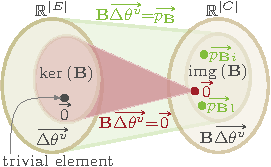
\includegraphics[scale=1,page=1]{networkAnalyzes/figures/ImageAndKernelOfALinearMapping.pdf}
    % 
    \vspace{-5mm}%
    \caption[The image and kernel of the circuit
    matrix~\glssymbol{cycleMatrix}.]{%
    % 
    The image~$\fimage{\glssymbol{cycleMatrix}}$ and kernel~$\fkernel{
    \glssymbol{cycleMatrix}}$ of the circuit matrix~\glssymbol{cycleMatrix} for
    the linear map~$
        % 
        \glssymbol{cycleMatrix}
        \colon
        \reals^{
            \fmagnitude{\glssymbol{edges}}
        }
        \to
        \reals^{
            \fmagnitude{\glssymbol{cycles}}
        }
        % 
    $.
    %
    }%
    % 
    \label{ch:network-analysis:fig:kernel-and-image-circuiteMatrix}%
    \vspace{-2mm}%
    % 
\end{wrapfigure}%
% 
\noindent homogeneous system~$
    % 
    \glssymbol{cycleMatrix}
    \cdot
    \vv{\glssymbol{voltageangledifference}} 
    =
    \vv{0}
    % 
$ holds for all vectors in that set
(see~\cref{ch:network-analysis:fig:kernel-and-image-circuiteMatrix} red area and
text). The image~$\fimage{
\glssymbol{cycleMatrix}}$ of the circuit matrix are all vectors~$
\frighthandsidevector{\glssymbol{cycleMatrix}}$ for which a solution exist 
(see~\cref{ch:network-analysis:fig:kernel-and-image-circuiteMatrix} green area
and text).

% , but a determinant
% of~$\pm 2^i$ with~$i\in\naturals$ and~$i$ being fix for a circuit
% matrix~\glssymbol{cycleMatrix}~\parencite{Oka55}. 
\noindent Using the rank-nullity theorem
(see~\cref{ch:network-analysis:def:rank-nullity-theorem}) 
we get the dimension of the kernel (nullity when talking about matrices) 
of~$
    % 
    \dimensionx{\fkernel{\glssymbol{cycleMatrix}}}
    =
    \dimensionx{\glssymbol{edges}}
    -
    \dimensionx{\fimage{\glssymbol{cycleMatrix}}}
    =
    \fmagnitude{\glssymbol{edges}} 
    - 
    \fmagnitude{\glssymbol{edges}} 
    +
    \fmagnitude{\glssymbol{vertices}} 
    - k
    =
    \fmagnitude{\glssymbol{vertices}} 
    - k
    % 
$.
 
\noindent However, \textcite{Ced55} showed that for a fundamental system of
circuits---that is used in our case---the determinant can only take values
of~$-1$, $0$, or $1$ for every square submatrix and~$\pm 1$ for a set of chords
that represents a maximal square matrix
(see~\cref{ch:network-analyzes:sec:mathematical-model:fig:TUM-proof}\screen{a}
or~\screen{b} bottom right partition). As for the incidence
matrix~\glssymbol{incidenceMatrix} above this means that the
matrix~\glssymbol{cycleMatrix} is~\gls{tum}.
% 
\begin{lemma}[\gls{tum} bases]
    The incidence matrix~\glssymbol{incidenceMatrix} and the
    circuit matrix~\glssymbol{cycleMatrix} are~\gls{tum} bases.
    % 
    \label{ch:network-analyzes:sec:mathematical-model:lem:I-and-B-TUM-sep}
\end{lemma}
%
\paragraph{Relationship between Incidence and Circuit Matrix}
\label{ch:network-analyzes:sec:mathematical-model:paragraph:relationsship-i-c-m}
% 
We get the relationship between the incidence matrix~\glssymbol{incidenceMatrix}
and the circuit matrix~\glssymbol{cycleMatrix}
in~\cref{ch:network-analyzes:sec:mathematical-model:eq:AB-orthogonality}.
% 
\begin{align}
    \glssymbol{incidenceMatrix}
    \transpose{\glssymbol{cycleMatrix}} 
    = 
    \mathbf{0}
    \quad
    % 
    \text{and}
    % 
    \quad
    \glssymbol{cycleMatrix}
    \transpose{\glssymbol{incidenceMatrix}} 
    = 
    \mathbf{0},
    % 
    \label{ch:network-analyzes:sec:mathematical-model:eq:AB-orthogonality}
\end{align}
% 
where~$\mathbf{0}$ is a matrix with zeros only of
dimension~$\fmagnitude{\glssymbol{vertices}}\times\fmagnitude{\glssymbol{cycles}}$
(respectively~$\fmagnitude{\glssymbol{cycles}}\times\fmagnitude{\glssymbol{vertices}}$).
Thus, the incidence matrix~\glssymbol{incidenceMatrix} is orthogonal to the
circuit matrix~\glssymbol{cycleMatrix}. One way to prove that is given
by~\textcite[p.66; Theorem 4-6]{Ses61} that uses the property of circuits that
have a degree of~$\degree(\vertexa) = 2$ at all
vertices~$\vertexa\in\glssymbol{vertices}$.
% 
Again note that both matrices~\glssymbol{incidenceMatrix}
and~\glssymbol{cycleMatrix} are orthogonal to each other (\ie, every vector
of~\glssymbol{incidenceMatrix} is orthogonal to every vector
in~\glssymbol{cycleMatrix}). Note that this also means that the vectors are
linear independent to each other. By doing a vertex transformation, we are able
to describe the voltage angle difference~$\glssymbol{voltageangledifference}
(\vertexa,\vertexc)$ vector by voltage angles~$\glssymbol{voltageangle}
(\vertexa)$ and~$\glssymbol{voltageangle}(\vertexc)$ for all
edges~$(\vertexa,\vertexc)\in\glssymbol{edges}$. However, this simple
transformation is based on the connection
that~$
    % 
    \glssymbol{cycleMatrix}
    \vv{\glssymbol{voltageangledifference}} 
    = 
    \vv{0}
    % 
$ and based on the relationship shown
in~\cref{ch:network-analyzes:sec:mathematical-model:eq:AB-orthogonality}.
% 
The connection given
in~\cref{ch:network-analyzes:sec:mathematical-model:eq:AB-orthogonality} allows
us to describe~$\vv{\glssymbol{voltageangledifference}}$ by the
linear combination of the tree branches~$
    % 
    \vv{\glssymbol{voltageangledifference}} 
    =
    \transpose{\glssymbol{incidenceMatrix}}
    \vv{\glssymbol{voltageangle}}
    % 
$ for each connected component (compare
also~\cref{ch:foundations:sec:power-flow-analyses:eq:assumption:vm:1,ch:network-analyzes:sec:mathematical-model:eq:kvl-ohm-function-writing}),
where~$
    % 
    \vv{\glssymbol{voltageangle}}
    \in 
    \reals^{\fmagnitude{\glssymbol{vertices}}-k}
    % 
$ with~$k$ representing the number of connected components~\parencite[Theorem
6-6, p. 123]{Ses61}. This means, we can find~$
    % 
    \glssymbol{cycleMatrix}
    \vv{\glssymbol{voltageangledifference}} 
    = 
    \vv{0}
    % 
$, which is equivalent of finding a~$
    % 
    \glssymbol{cycleMatrix}
    \transpose{\glssymbol{incidenceMatrix}}
    \vv{\glssymbol{voltageangle}} 
    = 
    \vv{0}
    % 
$. Since we know
from~\cref{ch:network-analyzes:sec:mathematical-model:eq:AB-orthogonality}
that~$
    % 
    \glssymbol{cycleMatrix}
    \transpose{\glssymbol{incidenceMatrix}} 
    =
    \mathbf{0}
    % 
$ this equation holds independent of the voltage angle
vector~$\vv{\glssymbol{voltageangle}}$. In addition, we would like to know when
there is a~$
    % 
    \vv{\glssymbol{voltageangle}}
    \in
    \reals^{
        \fmagnitude{\glssymbol{vertices}}
    }
    % 
$ such that~$
    % 
    \vv{\glssymbol{voltageangledifference}} 
    = 
    \transpose{
        \glssymbol{incidenceMatrix}
    }
    % \cdot
    \vv{\glssymbol{voltageangle}}
    % 
$. The latter is equivalent to the question of when~$
    % 
    \vv{\glssymbol{voltageangledifference}}
    \in
    \fimage{
        \transpose{\glssymbol{incidenceMatrix}}
    }
    % 
$. We have to show when~$
    % 
    \fkernel{\glssymbol{cycleMatrix}}
    \subseteq
    \fimage{\transpose{\glssymbol{incidenceMatrix}}}
$. This is the case when we chose the same spanning tree to construct both
matrices. Note that it suffices to compute the voltage angle differences along
a spanning tree, since the others result from these voltage angles.
% 
\paragraph{\gls{kvl} Flow}
\label{ch:network-analyzes:sec:mathematical-model:paragraph:kvl-flow}
% 
Applying the latter to Ohm's law gives us the typical equation
known from literature
(\cref{ch:network-analyzes:sec:mathematical-model:eq:kvl-ohm-function-writing}).
%
\begin{align}
    \glssymbol{susceptance}(\vertexa,\vertexc)
    \cdot
    \big(\glssymbol{voltageangle}(\vertexc)
    -
    \glssymbol{voltageangle}(\vertexa)
    \big) = \glssymbol{flow}(\vertexa,\vertexc).
    % 
    \label{ch:network-analyzes:sec:mathematical-model:eq:kvl-ohm-function-writing}
\end{align}
%
A flow~\glssymbol{flow} complying
with~\cref{ch:network-analyzes:sec:mathematical-model:eq:kvl-ohm-function-writing}
is called~\emph{\gls{kvl} flow} and if it complies with the capacity constraint
it is called~\emph{feasible~\gls{kvl} flow}. 

Using the aforementioned relationship
(\cref{ch:network-analyzes:sec:mathematical-model:eq:kvl-ohm-function-writing}),
we can
reformulate~\cref{ch:network-analyzes:sec:mathematical-model:eq:kvl-matrix-writing}
such that we replace voltage angle
differences~$\vv{\glssymbol{voltageangledifference}}$ by
flows~$\vv{\glssymbol{flow}}$. Note that~$
    % 
    \glssymbol{susceptance}(\vertexa,\vertexc)
    = 
    \nicefrac{ 1 }{ \glssymbol{reactance}(\vertexa,\vertexc) }
    % 
$ and that~\textquote{$\circ$} is the Schur product (or entrywise product). 
% 
\begin{subequations}
% 
\begin{align}
    % 
    \vv{\glssymbol{flow}} 
    = 
    \vv{\glssymbol{susceptance}} 
    \circ 
    \vv{\glssymbol{voltageangledifference}} 
    % 
    &\Leftrightarrow
    % 
    \hspace{2.35mm}
    \vv{\glssymbol{voltageangledifference}} 
    = 
    \vv{\glssymbol{reactance}} 
    \circ 
    \vv{\glssymbol{flow}} 
    \\
    \glssymbol{cycleMatrix}
    \vv{\glssymbol{voltageangledifference}} 
    = 
    \vv{0}\hspace{10mm}
    % 
    &\Leftrightarrow
    % 
        \underbrace{
            \left(
                \glssymbol{cycleMatrix}
                \circ    
                    (
                        \mathbb{1}^{ 
                            \fmagnitude{\glssymbol{edges}} 
                            \times 
                            1 
                        }
                        \cdot
                        \transpose{ \vv{\glssymbol{reactance}} }
                    )
            \right)
        }_{
            \eqqcolon
            \glssymbol{cycleMatrix}'
        }
    \cdot
    \vv{\glssymbol{flow}} 
    = 
    \vv{0}
    % 
    \label{ch:network-analyzes:sec:mathematical-model:eq:voltage-angle-diff-replacement-to-flows}
    % 
\end{align}
\label{ch:network-analyzes:sec:mathematical-model:eq:voltage-angle-diff-replacement-to-flows:allg}
\end{subequations}
% 
Since~$\vv{\glssymbol{reactance}}$ is a vector of constant values, we just
multiply the entries in the circuit matrix~$\glssymbol{cycleMatrix}$ by~$\vv{
\glssymbol{reactance}}$ resulting in a new circuit matrix~$
\glssymbol{cycleMatrix}'$, which results in~\cref{ch:network-analyzes:sec:mathematical-model:eq:voltage-angle-diff-replacement-to-flows:main}.
% 
\begin{align}
    \glssymbol{cycleMatrix}'
    \cdot
    \vv{\glssymbol{flow}}
    =
    \vv{0}
    % 
    \label{ch:network-analyzes:sec:mathematical-model:eq:voltage-angle-diff-replacement-to-flows:main}
    % 
\end{align}
% 
% 
\paragraph{Feasible Electrical Flow}
\label{ch:network-analyzes:sec:mathematical-model:paragraph:feasible-electrical-flow}
% 
In the following, we define feasible electrical flows that represent solutions
to~\gls{dc}~\gls{feas}.
% 
\begin{definition}[Feasible Electrical Flow]
    A~\gls{kvl} flow that is also a~\gls{kcl} flow is called~\emph{electrical
    flow} and if it complies to the capacity constraint, too, it is
    called a~\emph{feasible electrical flow}.
    % 
    \label{ch:network-analyzes:sec:mathematical-model:def:kvl-kcl-feasible-flow}
\end{definition}
% 
\gls{dc}~\gls{feas} and~\gls{dc}~\gls{mpfp} constitute a system of linear
equations and an~\gls{lp}, respectively. In the following, we summarize the
problem definitions of~\gls{dc}~\gls{feas} and~\gls{mpfp}.
% 
\begingroup
    %%%%%%%%%%%%%%%%%%%%%%%%%%%%%%%%%%% Problem %%%%%%%%%%%%%%%%%%%%%%%%%%%%%%%%%%%%
\begin{problem}[framed]{\acrlong{dc} \acrlong{feas} \gls{dc}-\gls{feas}$
(\glssymbol{network})$}%
  Instance: & An exact bounded network~\dcnetworktuple, \ie,
  $
  % \forall\vertex\in\glssymbol{generators}
  % \colon
  \glssymbol{realpowergeneration}
  \equiv
  \glssymbol{realpowergenerationmin}
  \equiv
  \glssymbol{realpowergenerationmax}$
  and~$
  % \forall
  % \vertex\in\glssymbol{consumers}
  % \colon
  \glssymbol{realpowerdemand}
  \equiv
  \glssymbol{realpowerdemandmin}
  \equiv
  \glssymbol{realpowerdemandmax}
  % 
  $.
  \\
  % 
  Question: & Is there a feasible electrical flow~\glssymbol{flow}
  (see~\cref{ch:network-analyzes:sec:mathematical-model:eq:kcl-matrix-writing,ch:network-analyzes:sec:mathematical-model:eq:kvl-matrix-writing,ch:network-analyzes:sec:mathematical-model:eq:capacity-constraint})?
  % ch:network-analyzes:sec:mathematical-model:eq:kvl-ohm-function-writing
\end{problem}%
    \label{ch:networkAnalysis:problems:DC_FEAS_Exact-Decision_Problem}
\endgroup
% 
A feasible electrical flow that maximizes the flow value~$
\glssymbol{flowvalue}(\glssymbol{network},\glssymbol{flow})
\coloneqq 
\sum_{\vertexa\in\glssymbol{generators}}
\glssymbol{netflow}(\vertexa)
$
is called~$\gls{mpfp}(\glssymbol{network})$ and its value is denoted
by~$\opt_{\gls{mpfp}}(\glssymbol{network})$. The optimization problem is stated
in the following.
%
\begingroup
    %%%%%%%%%%%%%%%%%%%%%%%%%%%%%%%%%%% Problem %%%%%%%%%%%%%%%%%%%%%%%%%%%%%%%%%%%%
\begin{problem}[framed]{\acrlong{dc} \acrlong{mpfp}~\gls{dc}-\gls{mpfp}%
$(\glssymbol{network})$}%
  Instance: & A network~\dcnetworktuple.\\
  % 
  Objective: & Find a feasible electrical flow~\glssymbol{flow}
  (see~\cref{ch:network-analyzes:sec:mathematical-model:eq:kcl-matrix-writing,ch:network-analyzes:sec:mathematical-model:eq:kvl-matrix-writing,ch:network-analyzes:sec:mathematical-model:eq:capacity-constraint}) 
  % ch:network-analyzes:sec:mathematical-model:eq:kvl-ohm-function-writing
  such that the flow value~$\glssymbol{flowvalue}(\glssymbol{network})$ is
  maximum among all choices of~\glssymbol{flow}.
\end{problem}%
    \label{ch:networkAnalysis:problems:DC_MPF-Decision_Problem}
\endgroup
%
\paragraph{Algorithms to Solve~DC~FEAS}%
\label{ch:network-analyzes:sec:mathematical-model:paragraph:algos-dc-feas}%
% 
Possibilities to get a feasible power flow are to formulate the system of linear
equations or~\gls{lp} and run it using a solver such as
Gurobi~\parencite{gurobi}, or to apply the following algorithm.
% 
\begin{lemma}[{{\textcite[p.36; Lemma 1]{Sha87}}}]
    Let every edge of~\glssymbol{graph} have a resistance~$\resistance\equiv 1$.
    Let~$\tree$ denote the number of spanning trees and
    let~$
        % 
        \tree(\source,\vertexa\rightarrow\vertexc,\sink)
        % 
    $ be the number of spanning trees that contain the
    edge~$(\vertexa,\vertexc)$ in that particular direction meaning the spanning
    tree has a path from~\source to~\sink that visits vertex~\vertexa first and
    then vertex~\vertexc by using the edge~$
        % 
        (\vertexa,\vertexc)
        \in
        \glssymbol{edges}
        % 
    $. Let~$
        % 
        \glssymbol{realpowergeneration}
        \equiv
        \glssymbol{realpowerdemand}
        \equiv 
        1
        % 
    $ and let~$
        % 
        \glssymbol{flow}(\vertexa,\vertexc)
        =
        \nicefrac{
            \big(
                \tree(\source,\vertexa\rightarrow\vertexc,\sink)
                -
                \tree(\source,\vertexc\rightarrow\vertexa,\sink)
            \big)
        }{
            \tree
        } 
        % 
    $. Then~\glssymbol{flow} is a feasible electrical flow in~\glssymbol{graph}.
    % 
    % Then~$\glssymbol{flow}(\vertexa,\vertexc)$ is the flow on the edge~$
    % (\vertexa,\vertexc)\in\glssymbol{edges}$ oriented from~\vertexa to~\vertexc.
    % 
    \label{ch:network-analyzes:sec:mathematical-model:lem:current_edge_from_a_to_b}
    % 
\end{lemma}
% 
The generalization---where we have no unit resistances~\glssymbol{resistance}, 
but arbitrary ones---given by~\textcite[p.38]{Sha87} was already given
by~\textcite[pp.155ff.]{Ses61}. Instead of just using the number of spanning
trees, we calculate for each spanning tree the product of the admittances of the
branches of that spanning tree and sum over all spanning trees. The proof of the
lemma uses the Binet-Cauchy-Theorem~\parencite[p.32]{Ses61}. Note that a graph
can have exponentially many spanning trees and computing the flow for each edge
using this techniques is quite inefficient, but provides an exponential time
algorithm to compute the electrical flow of the power grid.
% 
%%%%%%%%%%%%%%%%%%%%%%%%%%%%%%%%%%%%%%%%%%%%%%%%%%%%%%%%%%%%%%%%%%%%%%%%%%%%%%%%
\subsection{Properties of Electrical Flows}%
\label{ch:network-analyzes:sec:mathematical-model:properties-elec-flows}%
%%%%%%%%%%%%%%%%%%%%%%%%%%%%%%%%%%%%%%%%%%%%%%%%%%%%%%%%%%%%%%%%%%%%%%%%%%%%%%%%
% 
Note that we use a base for the columns of the incidence and circuit matrix
denoted by~\glssymbol{incidenceMatrix} and~\glssymbol{cycleMatrix},
respectively, where all equations are linear independent. Since the whole system
of equations has full rank the solution to a feasible electrical flow is unique,
which we show in the following.
%
\begin{lemma}[Uniqueness of \gls{dc} Electrical Flows]
    % 
    There is a unique solution to~\gls{dc} electrical flows if we have exact
    bounds.
    % 
    % lower bounds for generation~$\realpowergenerationmin$ and
    % demand~$\realpowerdemandmin$ are unbounded, and if such a solution exists.
    % 
    \label{ch:network-analyzes:sec:mathematical-model:lem:unique-flow}
    % 
\end{lemma}
% 
\begin{proof}
%
Recall that the incidence matrix~\glssymbol{incidenceMatrix} with~$
    % 
    \glssymbol{incidenceMatrix} 
    \in
    \reals^{
    (\fmagnitude{\glssymbol{vertices}} 
    - k)
    \times
    \fmagnitude{\glssymbol{edges}}}
    % 
$ and the circuit matrix~\glssymbol{cycleMatrix} with~$
    % 
    \glssymbol{cycleMatrix}
    \in
    \reals^{
    ( \fmagnitude{\glssymbol{edges}} 
    - \fmagnitude{\glssymbol{vertices}} 
    + k)
    \times
    \fmagnitude{\glssymbol{edges}}}
    % 
$ are bases. Since both matrices are bases the vectors are linear independent
in each matrix (\ie, this is a property of a base shown
in~\cref{ch:network-analyzes:sec:mathematical-model:eq:kvl-matrix-writing,ch:network-analyzes:sec:mathematical-model:eq:kcl-matrix-writing:1}).
% 
We now define a matrix~\constraintmatrix by~$
    % 
    \constraintmatrix 
    \coloneqq
    \binom{
        \glssymbol{incidenceMatrix}
    }{
        \glssymbol{cycleMatrix}'
    }
    % 
$ with~$\glssymbol{cycleMatrix}'$ from~\cref{ch:network-analyzes:sec:mathematical-model:eq:voltage-angle-diff-replacement-to-flows:main},
where~$
    % 
    \constraintmatrix
    \in
    \reals^{\fmagnitude{\glssymbol{edges}}\times\fmagnitude{\glssymbol{edges}}}
    % 
$ can be generalized to a linear map~$
    % 
    \constraintmatrix
    \colon
    \reals^{ \fmagnitude{ \glssymbol{edges} } }%
    \to
    \reals^{ \fmagnitude{ \glssymbol{edges} } }%
    % 
$ with~$
    % 
    \vv{ \glssymbol{flow} }%
    \mapsto%
    \constraintmatrix%
    \cdot%
    \vv{\glssymbol{flow}}%
    % 
$. Thus, the system of equations is defined by~$
    % 
    \constraintmatrix
    \cdot
    \vv{\glssymbol{flow}} 
    = 
    \frighthandsidevector{\constraintmatrix} 
    \coloneqq 
    \binom{
        \frighthandsidevector{\glssymbol{incidenceMatrix}}
    }{
        \vv{0}
    }
    % 
$ with vector~$\vv{0}$ of size~$
% 
\fmagnitude{\glssymbol{cycles}}
% 
$.
% 
The kernel~$\fkernel{\constraintmatrix}$ and the
image~$\fimage{\constraintmatrix}$ of matrix~\constraintmatrix are defined
in~\cref{ch:network-analysis:eq:constraintmatrix-matrix-image-and-kernel}.
%
\begin{subequations}
% 
\begin{align}
    % 
    \fkernel{\constraintmatrix}
    &
    \coloneqq 
    \{
        \vv{\glssymbol{flow}}
        \in
        \reals^{\fmagnitude{\glssymbol{edges}}}
        \mid 
        \constraintmatrix
        \cdot
        \vv{\glssymbol{flow}} 
        = 
        \vv{0}
    \} 
    &
    \subseteq
    \reals^{\fmagnitude{\glssymbol{edges}}}
    % 
    \label{ch:network-analysis:eq:constraintmatrix-matrix-kernel}
    % 
    \\
    % 
    \fimage{\constraintmatrix}
    &
    \coloneqq 
    \{
        \frighthandsidevector{\constraintmatrix} 
        \in
        \reals^{\fmagnitude{\glssymbol{edges}}}
        \mid 
        \exists
        \vv{\glssymbol{flow}}
        \in
        \reals^{\fmagnitude{\glssymbol{edges}}}
        \colon 
        \constraintmatrix
        \cdot
        \vv{\glssymbol{flow}} 
        = 
        \frighthandsidevector{\constraintmatrix} 
    \} 
    &
    \subseteq
    \reals^{\fmagnitude{\glssymbol{edges}}}
    % 
    \label{ch:network-analysis:eq:constraintmatrix-matrix-image}
    % 
\end{align}
\label{ch:network-analysis:eq:constraintmatrix-matrix-image-and-kernel}
\end{subequations} 
% 
From~\cref{ch:network-analyzes:sec:mathematical-model:eq:AB-orthogonality}, we
know that~$
    % 
    \glssymbol{incidenceMatrix} 
    \transpose{\glssymbol{cycleMatrix}} 
    =
    \mathbf{0}
    $ and~$
    \glssymbol{cycleMatrix} 
    \transpose{\glssymbol{incidenceMatrix}}
    =
    \mathbf{0}
    % 
$, which means that the dimension of the image of~\constraintmatrix is the sum
of the dimension of the images of the incidence matrix~\glssymbol{incidenceMatrix}
and circuit matrix~\glssymbol{cycleMatrix} given by~$
    % 
    \dimensionx{\fimage{\constraintmatrix}} 
    = 
    \dimensionx{\fimage{\incidenceMatrix}} 
    +
    \dimensionx{\fimage{\cycleMatrix}}  
    =
    \fmagnitude{\glssymbol{vertices}} - k
    +
    \fmagnitude{\glssymbol{edges}} - \fmagnitude{\glssymbol{vertices}} + k
    =
    \fmagnitude{\glssymbol{edges}}
    % 
$.
Using the rank-nullity theorem
(see~\cref{ch:network-analysis:def:rank-nullity-theorem}), we know that the
dimension of the kernel is~$\dimensionx{\fkernel{\constraintmatrix } } = 0$. 
Thus, \constraintmatrix as linear map is injective.
% 
% Now
% we consider two cases:
% % 
% \begin{compactenum}
%     \item If~$
%         \frighthandsidevector{\constraintmatrix} 
%         \not\in
%         \fimage{\constraintmatrix}
%     $, then the system has no solution.
%     % 
%     \item If~$
%         \frighthandsidevector{\constraintmatrix} 
%         \in
%         \fimage{\constraintmatrix}
%     $ there are two cases
%         \begin{compactenum}
%             \item $\dimensionx{\fimage{\constraintmatrix}} 
%                     < 
%                     \dimensionx{\glssymbol{edges}},$
%             \item $\dimensionx{\fimage{\constraintmatrix}} 
%                     = 
%                     \dimensionx{\glssymbol{edges}}.$
%         \end{compactenum}
% \end{compactenum}
% 
The dimension of the image of~\constraintmatrix is~$\fmagnitude{\edges}$, which
means that the matrix has full rank. We conclude that the system has a unique
non-trivial solution (see~\cref{ch:network-analyzes:fig:polytope-simple-example}).
% 
\end{proof}
%
% 
\begin{wrapfigure}{l}{6.5cm}% 
    \vspace{-0.6cm}
    % 
    \resizebox{6.35cm}{!}{%
\begin{tikzpicture}
\usepgfplotslibrary{fillbetween}
\usetikzlibrary{patterns}
\usetikzlibrary{intersections}
% pure inductive load
\begin{axis}[
    width=8.5cm,
    height=6.115cm,
    axis x line=middle, % center
    axis y line=middle, %none
    axis on top,
    domain=-4:7,
    xticklabels={$-4$, $-3$, $-2$, $-1$, $0$, $1$, $2$, $3$, $4$}, %\empty,
    xtick={-4.0, -3.0, -2.0, -1.0, 0, 1.0, 2.0, 3.0, 4.0},
    yticklabels={$-3$, $-2$, $-1$, $0$, $1$, $2$, $3$}, %
    ytick={-3.0, -2.0, -1.0, 0, 1.0, 2.0, 3.0},
    x tick style={color=KITblack70, thick,line cap=round},
    y tick style={color=KITblack70, thick,line cap=round},
    minor y tick num=1,
    minor x tick num=1,
    samples=1001,
    xlabel={$x$},
    ylabel={$y$},
    legend pos=outer north east,
    xmin=-4.0-0.5,
    xmax=4.0+0.5,
    ymin=-3.0-0.5,
    ymax=3.0+0.5,
    axis line style={KITblack70, thick}, %line cap=round, 
    x tick label style={font=\color{KITblack70}},
    y tick label style={font=\color{KITblack70}},
every axis x label/.style={
    at={(ticklabel* cs:1.0)},
    anchor=west,
},
every axis y label/.style={
    at={(ticklabel* cs:0.98)},
    anchor=south,
},
    x label style={font=\color{KITblack70}},
    y label style={font=\color{KITblack70}},
    % set clip=false to avoid clipping of nodes
    clip=false,
]
%
% Gray vertical lines
% 
    \def \xMin {-5.0}
    \def \xMax {5.0}
    \def \yMin {-4.0}
    \def \yMax {4.0}
%
% y cut at one
%
    \def \yBounded {1}
    % 
    \addplot[name path=fctYmax, mark=none, draw=none, line cap=round] 
    coordinates {(\xMin, 3.0 ) (\xMax, 3.0 )};
    % 
    \addplot[name path=fctYmin, mark=none, draw=none, line cap=round] 
    coordinates {(\xMin, -3.0 ) (\xMax, -3.0 )};
    % 
    \addplot[name path=fctXmin, mark=none, draw=none, line cap=round] 
    coordinates {(-4.0, \yMin ) (-4.0, \yMax )};
    % 
    \addplot[name path=fctXmax, mark=none, draw=none, line cap=round] 
    coordinates {(4.0, \yMin ) (4.0, \yMax )};
    % 
%
% Functions Representing the Simple "Hyperplanes", i.e., Straights
%
    \def \fctRed { -1 * x + 3 }
    \def \fctBlue { 1 * x - 1 }
    \def \fctDarkGreen { 3/2 * x + 3 }
    \def \fctLightGreen { -1/2 * x - 2 }
    % 
    % \newcommand{\drawge}{-- (rel axis cs:1,0) -- (rel axis cs:1,1) -- (rel axis cs:0,1) \closedcycle}
    % \newcommand{\drawle}{-- (rel axis cs:1,1) -- (rel axis cs:1,0) -- (rel
    % axis cs:0.01,0) \closedcycle}
    % 
    \addplot [name path=fctRed, domain = -0.5:5.1, ultra thick, KITred70, line
    cap=round] 
    {\fctRed} node[above,right,pos=1.0] {$ y = -x + 3$}; 
    % 
    \addplot [name path=fctBlue, domain = -2.5:4.1, ultra thick, KITseablue70,
    line cap=round] 
    {\fctBlue} node[above,right,pos=1.0] {$ y = x - 1$}; 
    % 
    \addplot [name path=fctDarkGreen, domain = -4.1:0.5, ultra thick,
    KITgreen70, line cap=round, fill=black]
    {\fctDarkGreen} 
    node[above,right,pos=0.98] 
    {$y = \nicefrac{3}{2} x + 3$};
    % 
    \addplot [name path=fctLightGreen, domain = -5.0:3.1, ultra thick,
    KITcyanblue70, line cap=round] 
    {\fctLightGreen} 
    node[above,right,pos=1.0] 
    {$y = -\nicefrac{x}{2} - 2$};
    %
    \addplot [line width=1pt,fill=KITcyanblue70,draw=none,fill opacity=0.08] 
    fill between[
            of=fctLightGreen and fctYmax,
            soft clip={domain=-5:5},
    ];
    % \addplot [draw=none, fill=KITseablue70,fill
    % opacity=0.908, domain=-4.5:\xMax]{\fctLightGreen} \drawge; 
    % \addplot [draw=none, fill=KITgreen70,fill
    % opacity=0.908, domain=-4.4:\xMax]{\fctDarkGreen} \drawle;
    % \addplot [draw=none, fill=KITgreen70,fill
    % opacity=0.908, domain=-4:\xMax]{\fctDarkGreen} \drawle; 
    % \addplot [draw=none, pattern=north west lines, pattern color=blue!40, domain=-10:12]
    %          {-5+2*x} \drawge;
    % \addplot [draw=none, pattern=horizontal lines, pattern color=blue!40, domain=-10:10]
    %          {3/2+x/2} \drawle; 
    % 
    \addplot [line width=1pt,fill=KITseablue70,draw=none,fill opacity=0.08] 
    fill between[
            of=fctBlue and fctXmin,
            soft clip={domain=-5:5},
    ];
    % 
    \addplot [line width=1pt,fill=KITred70,draw=none,fill opacity=0.08] 
    fill between[
            of=fctRed and fctYmin,
            soft clip={domain=-5:5},
    ];
    % 
    \addplot [line width=1pt,fill=KITgreen70,draw=none,fill opacity=0.08] 
    fill between[
            of=fctDarkGreen and fctXmax,
            soft clip={domain=-5:5},
    ];
    % 
    % 
%
% Cut Area of the four functions
%
    \addplot [line width=1pt,fill=orange,draw=none,fill opacity=0.2] 
    coordinates{
        (0,3) 
        (2,1) 
        (-2/3,-5/3) 
        (-5/2,3/2*-5/2+3)
    } node[above,pos=0.3,orange] {$\polyhedron$};
    % 
    \addplot [line width=1pt,fill=KITlilac70,draw=KITlilac70,fill opacity=0.2] 
    (-2/3,-5/3) circle (1ex);%
    %
    \addplot[mark=none, KITpalegreen, dashed, line cap=round] 
    coordinates {(\xMin, \yBounded ) (4.0, \yBounded )}
    node[right,pos=1.0]{$y$ is fixed to~$1$};
%
\end{axis}
\end{tikzpicture}
}%
    % 
    % \vspace{-0.05cm}
    % 
    \caption[A simple polytope example.]{The \textcolor{orange!60}
    {Polytope~\polyhedron} constituted by~$
    % 
     \textcolor{KITgreen70}{y \leq \nicefrac{3}{2} x + 3}$,
    % 
    $\textcolor{KITseablue70}{y \geq x - 1}$, 
    % 
    $\textcolor{KITred70}{y \leq -x + 3}$, and~$
    % 
     \textcolor{KITcyanblue70}{y \geq -\nicefrac{x}{2} - 2}$. 
    % 
    If~$\textcolor{KITpalegreen70}{y = 1}$, we reduce the solution space
    to~$x\in[-\nicefrac{4}{3}, 2]$. However, if~$y = -\nicefrac{5}{3}$ the
    solution is unique~$x = -\nicefrac{2}{3}$. So a unique solution corresponds
    to one point~\tikzPolytopePoint.
    % 
    % 
    }%
    \vspace{-0.4cm}
    % 
    \label{ch:network-analyzes:fig:polytope-simple-example}%
\end{wrapfigure}%
%  
Note that the system has no non-trivial solution if the generations and demands
are exact and the capacities are chosen in such a way that these generations and
demands cannot be fulfilled. In the following, we extend the system by capacity
constraints discussed
in~\cref{ch:network-analyzes:sec:mathematical-model:eq:capacity-constraint}.% We ask if the system with the capacity constraints has still full rank.
% 

The capacity constraint can be reformulated in a matrix writing by~$
    % 
    {\mathbb 1}^{
        \fmagnitude{ \glssymbol{edges} } 
        \times
        \fmagnitude{ \glssymbol{edges} } 
    }
    \cdot
    \vv{\glssymbol{flow}}
    \leq
    \vv{\glssymbol{capacity}}
    % 
$, where~$
    % 
    {\mathbb 1}^{ 
        \fmagnitude{\glssymbol{edges} } 
        \times 
        \fmagnitude{\glssymbol{edges} } 
    }
    % 
$ is the identity matrix of size~$
    % 
    \fmagnitude{ \glssymbol{edges} }
    \times
    \fmagnitude{ \glssymbol{edges} }
    % 
$ and the vector of capacities is~$
    % 
    \vv{ \glssymbol{capacity} } 
    \in 
    \reals^{
        \fmagnitude{
            \glssymbol{edges}
        }
    }
    % 
$. With the capacity constraint we get a matrix~$
    % 
    \constraintmatrix' 
    = 
    \transpose{
    (
        \glssymbol{incidenceMatrix}, 
        \glssymbol{cycleMatrix}', 
        {\mathbb1}^{
            \fmagnitude{\glssymbol{edges} } 
            \times
            \fmagnitude{\glssymbol{edges} } 
        }
    )
    }
    % 
$ of size~$
    % 
    \constraintmatrix'
    \in
    \reals^{
        ( 2\fmagnitude{\glssymbol{edges}} )
        \times
        \fmagnitude{\glssymbol{edges}}
    } 
    % 
$ with~$\glssymbol{cycleMatrix}'$ 
from~\cref{ch:network-analyzes:sec:mathematical-model:eq:voltage-angle-diff-replacement-to-flows:main}.
Note that the additional submatrix has no influence on the dimension of the
image meaning~$
    % 
    \dimensionx{\fimage{\constraintmatrix'}} 
    = 
    \fmagnitude{\glssymbol{edges}}
    % 
$, \ie, using the rank-nullity-theorem
(\cref{ch:network-analysis:def:rank-nullity-theorem}), we get the dimension of
the kernel~$
    % 
    \dimensionx{\fkernel{\constraintmatrix}} = 0
    % 
$. The matrix remains to have a full rank, but we have inequality constraints.
With exact supplies (\ie, $
    % 
    \glssymbol{realpowergeneration}
    \equiv
    \glssymbol{realpowergenerationmin}
    \equiv
    \glssymbol{realpowergenerationmax}
    % 
$) and exact demands (\ie, $
    % 
    \glssymbol{realpowerdemand}
    \equiv
    \glssymbol{realpowerdemandmin}
    \equiv
    \glssymbol{realpowerdemandmax}
    % 
$) the capacity constraints have only influence on the feasibility of a
solution, since~$
    % 
    \constraintmatrix 
    \cdot 
    \vv{\glssymbol{flow}} 
    = 
    \frighthandsidevector{\constraintmatrix} 
    % 
$ gives us a unique solution the inequality~$
    % 
    \mathbb{1}^{ 
        \fmagnitude{\glssymbol{edges}} 
        \times 
        \fmagnitude{\glssymbol{edges}} 
    }
    \cdot
    \vv{\glssymbol{flow}}
    \leq
    \vv{\glssymbol{capacity}}
    % 
$ might lead to a polytope that does not include that solution.

If we apply upper bounds~$\frighthandsidevector{\constraintmatrix\uparrow}$
with~$
    % 
    \glssymbol{realpowergenerationmax}, 
    \glssymbol{realpowerdemandmax}
    \in
    \posreals
    % 
$, and lower bounds~$\frighthandsidevector{\constraintmatrix\downarrow}$ with~$
    % 
    \glssymbol{realpowergenerationmin}, 
    \glssymbol{realpowerdemandmin}
    \in
    \posreals
    % 
$ for the generations and demands, we get the following system of
inequalities.
% 
\begin{subequations}
\begin{align}
    % 
    \hphantom{-}\constraintmatrix
    \cdot
    \vv{\glssymbol{flow}} 
    % 
    &\leq
    % 
    \hphantom{-}\frighthandsidevector{\constraintmatrix\uparrow} 
    % 
    \label{ch:network-analysis:eq:upper-bounds}
    % 
    \\
    % 
    -\constraintmatrix
    \cdot
    \vv{\glssymbol{flow}} 
    % 
    &\leq
    % 
    -\frighthandsidevector{\constraintmatrix\downarrow} 
    % 
    \label{ch:network-analysis:eq:lower-bounds}
    % 
\end{align}
\label{ch:network-analysis:eq:lower-and-upper-bounds}
\end{subequations}
% 
Without capacities, if we set the bound for each~$
\frighthandsidevector{\constraintmatrix}$
between~$
    % 
    \frighthandsidevector{\constraintmatrix\uparrow}
    % 
$ and~$
    % 
    \frighthandsidevector{\constraintmatrix\downarrow} 
    % 
$ (see~\cref{ch:network-analysis:eq:lower-and-upper-bounds}) to exact, we would
get a unique solution. Otherwise, this set of solution can be represented by a
polytope that is no longer just a point, but defined by the faces~$\cuts_{i}$
that build a convex hull. However, while maximized, we can simply use the upper
bound vector~$\frighthandsidevector{\constraintmatrix\uparrow}$. Thus, the
solution for the~\gls{mpfp} is still unique. Note that this is no longer true
when we add capacity constraints.
% 
\begin{lemma}[Uniqueness of~\gls{mpfp}]
    % 
    There is a unique solution to (feasible)~\gls{dc} electrical flows, when
    maximized as long as there are no capacity constraints.
    % 
\end{lemma}

% 
\begin{wrapfigure}{l}{4.5cm}%
    % 
    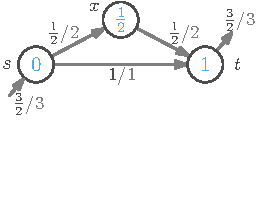
\includegraphics[scale=1,page=1]{networkAnalyzes/figures/tum_counter_example.pdf}
    % 
    \caption[\gls{tum} counter example.]{% 
        % 
        A~\gls{tum} counter example with three vertices with
        \textcolor{THETA}{voltage angles~\glssymbol{voltageangle}} that are
        written in the vertices, flows~\glssymbol{flow} and
        capacities~\glssymbol{capacity} are written on the edges~$
            % 
            \textcolor{KITblack70}{\glssymbol{flow}}
            /
            \textcolor{CAPACITY}{\glssymbol{capacity}}
            % 
        $. This example shows that flows are not necessarily integral, since the
        edges~$
            % 
            (\source, x), 
            (x,\sink)
            \in
            \glssymbol{edges}
            % 
        $ have each a flow of~$\textcolor{KITblack70}{\nicefrac{1}{2}}$.
        % \vspace{-15mm}
        % 
    }%
    %
    \label{ch:network-analyzes:fig:tum-counter-example}%
    % 
\end{wrapfigure}%
% 
Another application, where the rank of the matrix can be used is to check
whether a network with a given set of sensors is observable (\ie, all other
variables can be calculated by the measured ones). \textcite[p.487;(47)]{Kal59}
uses the property that if a set of vectors is linear independent then the system
becomes observable. Note that another way to prove the uniqueness was given
by~\textcite[p.114; Lemma 4.2.1]{Ver10} and~\textcite[p.361]{Roc84}.

\noindent A system of linear inequalities represents a convex polytope~$
    % 
    \polyhedron
    =
    \{
        \vv{\glssymbol{flow}} \in \reals^{\fmagnitude{ \glssymbol{edges} } }
        \mid
        \constraintmatrix
        \vv{ \glssymbol{flow} }
        \leq
        \frighthandsidevector{\constraintmatrix} 
    \}
    % 
$. Let~$\cuts_{i}$ be a hyperplane defined by~$
    % 
    \cuts_{i} 
    \coloneqq 
    \{
        \vv{\glssymbol{flow}}
        \in
        \reals^{ \fmagnitude{ \glssymbol{edges} } }
        \mid
        \constraintmatrix_i
        \cdot
        \vv{\glssymbol{flow}}
        =
        \frighthandsidevector{\constraintmatrix}_i 
    \}
    % 
$ that represents the~$i^{\mathrm{th}}$ row with~$
    % 
    1
    \leq 
    i
    \leq
    \fmagnitude{\glssymbol{edges}}
    % 
$. The cuts of a convex polytope~\polyhedron with each hyperplane~$\cuts_{i}$ is
given by~$
    % 
    \{
        \polyhedron
        \cap
        \cuts_{i}
        \mid
        1 \leq i \leq \fmagnitude{\glssymbol{edges}}
    \}
    % 
$ and represents the set of faces that form a \emph{convex hull}. 

Consider any objective then an optimal solution of a convex polytope~\polyhedron
is on the vertices of~\polyhedron. Thus, if the vertices of a convex
polytope~\polyhedron lie on integral coordinates than~\polyhedron is called
an~\emph{integral polytope}. If all square submatrices of~\constraintmatrix have
a determinant of~$-1, 0,$ or~$1$ then~\constraintmatrix is~\gls{tum}. This in
particular means that the polytope of such a~\gls{tum} matrix is integral
independent on the vector~$
    % 
    \frighthandsidevector{\constraintmatrix}
    % 
$.

Recall that we know that the incidence
matrix~\glssymbol{incidenceMatrix} and circuit matrix~\glssymbol{cycleMatrix}
are each~\gls{tum} by itself
(see~\cref{ch:network-analyzes:sec:mathematical-model:lem:I-and-B-TUM-sep}). In
the following, we prove that the whole system~$
    % 
    \constraintmatrix 
    \coloneqq 
    \binom{ 
        \glssymbol{incidenceMatrix} 
    }{ 
        \glssymbol{cycleMatrix} 
    }
    % 
$ is not~\gls{tum} and thus, the convex polytope is not necessarily integral.
% 
\begin{lemma}
% 
The bases of the incidence matrix~\glssymbol{incidenceMatrix} and the circuit
matrix~\glssymbol{cycleMatrix} are each~\gls{tum}. However, the whole system
of linear equations~$
% 
\constraintmatrix 
\coloneqq 
\binom{ 
    \glssymbol{incidenceMatrix} 
}{ 
    \glssymbol{cycleMatrix} 
}
% 
$ to compute a feasible electrical flow using the~\gls{kcl}
(\cref{ch:network-analyzes:sec:mathematical-model:eq:kcl-matrix-writing})
and~\gls{kvl}
(\cref{ch:network-analyzes:sec:mathematical-model:eq:kvl-matrix-writing}) is
not~\gls{tum}.
% 
\label{ch:network-analyzes:sec:mathematical-model:lem:pf-matrix-is-tum}
% 
\end{lemma}
% 
\begin{proof}
    % 
    A counter example is shown
    in~\cref{ch:network-analyzes:fig:tum-counter-example} that basically
    describes why a feasible electrical flow~\glssymbol{flow} is not integral
    for every right hand-side vector~$\frighthandsidevector{\constraintmatrix}$.
    % 
\end{proof}%

The~\gls{kcl}
(see~\cref{ch:network-analyzes:sec:mathematical-model:eq:kcl-matrix-writing})
and the~\gls{kvl}
(see~\cref{ch:network-analyzes:sec:mathematical-model:eq:kvl-matrix-writing}) do
not incorporate network elements in any sense---\ie, these equations are purely
topological~\parencite[p.127; Section 6-3]{Ses61}---the vector of voltage angle
differences~$\vv{\glssymbol{voltageangledifference}}$ can be replaced by the
flow vector~$\vv{\glssymbol{flow}}$. 

\begin{figure}
    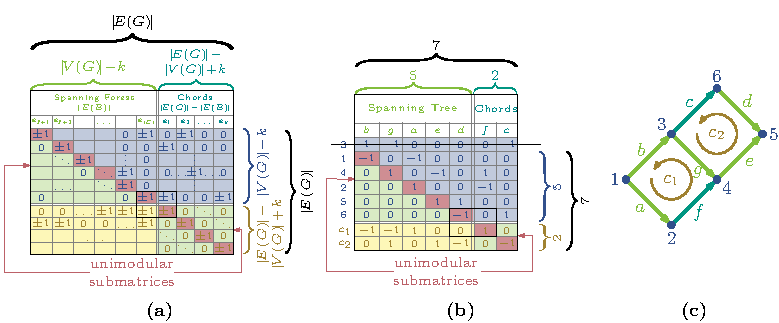
\includegraphics{networkAnalyzes/figures/Tum-proof.pdf}
     % 
    \caption[The combined incidence and circuit matrix structure.]{The structure
    of the matrix~$
    % 
        \constraintmatrix 
        \coloneqq 
        \binom{
            \textcolor{KITseablue}{\glssymbol{incidenceMatrix}}
        }{
            \textcolor{KITbrown}{\glssymbol{cycleMatrix}}
        }
    % 
    $ that is a construction of the \textcolor{KITseablue}{incidence
    matrix~\glssymbol{incidenceMatrix}} (top partition) and
    \textcolor{KITbrown}{circuit matrix~\glssymbol{cycleMatrix}} (bottom
    partition). The~\textcolor{KITpalegreen}{left partition} of
    size~$\textcolor{KITpalegreen}{\fmagnitude{\glssymbol{vertices}}-k}$,
    with~$k$ being the number of connected components (for (b) and (c) with one
    connected component~$k=1$), represents
    some~\textcolor{KITpalegreen}{spanning forest} (for $k=1$
    a~\textcolor{KITpalegreen}{spanning tree}) of the graph~\glssymbol{graph}.
    The~\textcolor{KITgreen}{right partition} represents the edges that are not
    in the~\textcolor{KITpalegreen}{spanning forest} of the left partition (also
    called~\textcolor{KITgreen}{chords}). The latter partition has a size
    of~$
        \textcolor{KITgreen}{%
            \fmagnitude{\glssymbol{edges}}%
            -
            \fmagnitude{\glssymbol{vertices}}%
            + k
        }%
        % 
    $. The green areas have entries that are all zero and the main diagonal with
    entries all~$\pm 1$ is marked in red. The general structure is given in (a)
    and a small example is given in (b) with the corresponding graph in (c).}%
    % 
    \label{ch:network-analyzes:sec:mathematical-model:fig:TUM-proof}%
\end{figure}
% 
Let~$\tree$ be a spanning tree in~$\glssymbol{graph}$. The
matrix~$
    % 
    \constraintmatrix
    \coloneqq
    \binom{
        % 
        \glssymbol{incidenceMatrix}_{%
            \glssymbol{edges}(\tree)%
        }\quad\glssymbol{incidenceMatrix}_{%
            \glssymbol{edges}(\glssymbol{graph})%
            \setminus%
            \glssymbol{edges}(\tree)%
        }% 
        % 
    }{
        % 
        \glssymbol{cycleMatrix}_{%
            \glssymbol{edges}(\tree)%
        }\quad\glssymbol{cycleMatrix}_{%
            \glssymbol{edges}(\glssymbol{graph})%
            \setminus%
            \glssymbol{edges}(\tree)%
        }%
        % 
    }
    % 
$ can be decomposed into two parts column-wise represented by the partitions
that are the set~$\glssymbol{edges}(\tree)$ of spanning tree edges
(see~\cref{ch:network-analyzes:sec:mathematical-model:fig:TUM-proof}\screen{a}
left top and bottom partition) and the set~$
    % 
    \glssymbol{edges}(\glssymbol{graph})
    \setminus
    \glssymbol{edges}(\tree)
    % 
$ of chords
(see~\cref{ch:network-analyzes:sec:mathematical-model:fig:TUM-proof}\screen{a}
right top and bottom partitions) for some arbitrary but fixed spanning
tree~\tree. The partition of the rows into two parts is given by construction~$
    % 
    \constraintmatrix
    =
    \binom{
        \glssymbol{incidenceMatrix}
    }{
        \glssymbol{cycleMatrix}
    }
    % 
$. Recall that all maximum square non-singular submatrices (\ie, matrices that
have a nonzero determinant) of the incidence
matrices~\glssymbol{incidenceMatrix} of size~$
    % 
    (\fmagnitude{\glssymbol{vertices}}-1)
    \times
    (\fmagnitude{\glssymbol{vertices}}-1)
    % 
$ are formed by some spanning tree~$\tree\in\mathcal T$ and submatrices of 
the
circuit matrix~\glssymbol{cycleMatrix} of size~$
    % 
    (\fmagnitude{\glssymbol{edges}} - \fmagnitude{\glssymbol{vertices}} + 1)
    \times
    (\fmagnitude{\glssymbol{edges}} - \fmagnitude{\glssymbol{vertices}} + 1)
    % 
$ that are formed by a set of chords, are unimodular (\ie, the
determinant is~$\pm 1$; 
see~\cref{ch:network-analyzes:sec:mathematical-model:fig:TUM-proof} top left
and bottom right partition, respectively). The structure allows us to permute
the entries such that the main diagonal has only~$\pm 1$ entries 
(see~\cref{ch:network-analyzes:sec:mathematical-model:fig:TUM-proof}\screen{a}
and~\screen{b} for example). We describe in the following how we permute the
matrix~\constraintmatrix.

We can order the rows and columns of the incidence
matrix~\glssymbol{incidenceMatrix} that are in the spanning tree partition
(see~\cref{ch:network-analyzes:sec:mathematical-model:fig:TUM-proof}\screen{a}
and~\screen{b} top left partition) such that entries below the diagonal are all
zero in that partition. This particular form of a matrix is denoted by the term
\emph{upper triangular matrix}. A property of the incidence
matrix~\glssymbol{incidenceMatrix} is that it has at most two non-zero entries
per column. In addition, the number of leaves~$
    % 
    \mathcal{L}
    \coloneqq
    {\{
        \vertexa
        \in
        \glssymbol{vertices}
        \mid
        \degree(\vertexa) 
        = 
        1
    \}}
    % 
$ in a spanning tree depend on the degree of the vertices meaning~$
    % 
    \fmagnitude{\mathcal{L}} 
    \geq
    \max_{\vertexa\in\glssymbol{vertices}}
    \degree (\vertexa)
    % 
$, which means that there is always enough space to the right of the diagonal.
To construct an upper triangular matrix in~\constraintmatrix
(see~\cref{ch:network-analyzes:sec:mathematical-model:fig:TUM-proof}\screen{a}),
we perform a~\acrlong{bfs} (\gls{bfs}). The~\gls{bfs} processes the inner
vertices of the spanning tree first and at the end all leaves. Using the
aforementioned observation of the number of leaves, we know that there is always
enough space to the right of the main diagonal. For the chord partition of the
circuit matrix~\glssymbol{cycleMatrix}, we are always able to adjust the entries
such that the lower and upper triangle of the matrix have zero entries only
(\cref{ch:network-analyzes:sec:mathematical-model:fig:TUM-proof}\screen{a}
and~\screen{b}; bottom right partition).
% 
We describe the~\gls{bfs} in the following.
 
Let~\tree be an arbitrary but fixed spanning tree and
let~\glssymbol{cycleMatrix} be the base of the columns of the circuit matrix
constructed from spanning tree~\tree. We start at some
vertex~$\vertexa\in\glssymbol{vertices}(\glssymbol{graph})$
(see~\cref{ch:network-analyzes:sec:mathematical-model:fig:TUM-proof}\screen{c}
vertex~$3$) and process its incident edges~$
    % 
    \{\vertexa,\vertexb\}
    \in
    \glssymbol{undirectededges}(\tree)
    % 
$. We add the columns of the incident edges to an empty
matrix~$\constraintmatrix'$ and the adjacent vertices~$
    % 
    \vertexb
    \in
    \glssymbol{vertices}(\glssymbol{graph})
    % 
$ as row. We proceed the aforementioned procedure with the next row's
vertex~\vertexb. Afterwards, we add the cycles~$\cycle\in\cycles$ that are in
the circuit matrix base~$\cycleMatrix$. Since each cycle in the base contributes
one nonzero chord entry, we add for each cycle the corresponding chord column~$
    % 
    \undirectededge
    \in
    \glssymbol{undirectededges}(\glssymbol{graph})
    \setminus
    \glssymbol{undirectededges}(\tree)
    % 
$. The resulting matrix is of the form~$
    % 
    \constraintmatrix'%
    \coloneqq%
    \binom{%
        % 
        \glssymbol{incidenceMatrix}_{%
            \glssymbol{edges}(\tree)%
        }\quad\glssymbol{incidenceMatrix}_{%
            \glssymbol{edges}(\glssymbol{graph})%
            \setminus%
            \glssymbol{edges}(\tree)%
        }% 
        % 
    }{%
        % 
        \glssymbol{cycleMatrix}_{%
            \glssymbol{edges}(\tree)%
        }\quad\glssymbol{cycleMatrix}_{%
            \glssymbol{edges}(\glssymbol{graph})%
            \setminus%
            \glssymbol{edges}(\tree)%
        }%
        % 
    }
    % 
$. We can conclude this discussion with the following lemma.
% 
\begin{lemma}
    % 
    Let~$
        % 
        \constraintmatrix 
        = 
        \binom{
            \glssymbol{incidenceMatrix}
        }{  
            \glssymbol{cycleMatrix}
        }
        % 
    $ be the matrix formed by the incidence matrix~\glssymbol{incidenceMatrix}
    and circuit matrix~\glssymbol{cycleMatrix}. The matrix's columns and rows
    can be permuted such that we get the form shown
    in~\cref{ch:network-analyzes:sec:mathematical-model:fig:TUM-proof}\screen{a}.
    % 
\end{lemma}
% 
To investigate the~\gls{tum} property, we take a look at the intersections of
the matrix~\constraintmatrix that are represented by all four partitions
(see~\cref{ch:network-analyzes:sec:mathematical-model:fig:TUM-proof}\screen{a}).
Thus, we distinguish between the following three main cases.
% 
\begin{compactenum}[\hspace*{3mm}\textbf{Case} 1\textbf{:}]
    % 
    \item The intersection between the chord and spanning tree partition of
    \label{ch:network-analyzes:sec:mathematical-model:cases:1}
    % 
    \begin{compactenum}[\hspace*{-11mm}(a)]
        % 
        \item the incidence matrix~\glssymbol{incidenceMatrix} (\cref{ch:network-analyzes:sec:mathematical-model:fig:TUM-proof}\screen{a}
        \&~\screen{b}; top left and top right partition),
        % 
        \label{ch:network-analyzes:sec:mathematical-model:cases:1a}
        % 
        \item the circuit matrix~\glssymbol{cycleMatrix} 
        (\cref{ch:network-analyzes:sec:mathematical-model:fig:TUM-proof}\screen{a}
        \&~\screen{b}; bottom left and bottom right partition).
        % 
        \label{ch:network-analyzes:sec:mathematical-model:cases:1b}
        % 
    \end{compactenum}
    % 
    \item The intersection between the incidence matrix~\glssymbol{incidenceMatrix}
    and the circuit matrix~\glssymbol{cycleMatrix} of
    \label{ch:network-analyzes:sec:mathematical-model:cases:2}
    % 
    \begin{compactenum}[\hspace*{-11mm}(a)]
        % 
        \item the spanning tree partition 
        (\cref{ch:network-analyzes:sec:mathematical-model:fig:TUM-proof}\screen{a}
        \&~\screen{b}; top left and bottom left partition), 
        % 
        \label{ch:network-analyzes:sec:mathematical-model:cases:2a}
        % 
        \item the chord partition 
        (\cref{ch:network-analyzes:sec:mathematical-model:fig:TUM-proof}\screen{a}
        \&~\screen{b}; top right and bottom right partition).
        % 
        \label{ch:network-analyzes:sec:mathematical-model:cases:2b}
        % 
    \end{compactenum}
    % 
    \item The intersection of all four partitions.
    \label{ch:network-analyzes:sec:mathematical-model:cases:3}
    % 
\end{compactenum}
% 
Since each matrix is~\gls{tum} by itself
Case~\ref{ch:network-analyzes:sec:mathematical-model:cases:1} is unproblematic
(see~\cref{ch:network-analyzes:sec:mathematical-model:lem:I-and-B-TUM-sep}). In
Case~\ref{ch:network-analyzes:sec:mathematical-model:cases:2}, we are already
able to find a square submatrix with determinant unequal~$\pm 1$ or~$0$
(see~\cref{ch:network-analyzes:sec:mathematical-model:fig:TUM-proof}\screen{b}
row~$5$ columns~$e$ and~$d$). 
% 
% In Case~\ref{ch:network-analyzes:sec:mathematical-model:cases:1a}, it is
% possible to get a submatrix where both diagonals are all~$\pm 1$. The latter
% case happens when there are multi-edges in the graph. These multi-edges have the
% property of being anti-symmetric and thus, the determinant is~$0$. For
% Case~\ref{ch:network-analyzes:sec:mathematical-model:cases:1b}, it is only
% possible that one diagonal is~$\pm 1$, since the chord matrix's triangles have
% only zero entries.
% 
% Now we come to Case~\ref{ch:network-analyzes:sec:mathematical-model:cases:2}. We
% start with the intersection of the two spanning tree partitions
% (Case~\ref{ch:network-analyzes:sec:mathematical-model:cases:2a}; left matrix
% partition
% in~\cref{ch:network-analyzes:sec:mathematical-model:fig:TUM-proof}\screen{a}).
% We mentioned above that we are always able to construct an incidence
% matrix~\glssymbol{incidenceMatrix} in such a way that the main diagonal of the
% matrix is~$\pm 1$ and that we get a triangle that has zero entries only either
% above or below the main diagonal
% (see~\cref{ch:network-analyzes:sec:mathematical-model:fig:TUM-proof}\screen{a}
% or~\screen{b}; green triangle in the top left partition). Thus, the only case
% where we get a diagonal is by using the last~$\pm 1$ entry of the main diagonal
% close to the intersection. However, since the other diagonal is always zero
% (since the triangle of~\glssymbol{incidenceMatrix} is all zero) these matrices
% are always unimodular. The same argument can be used for the chord section
% (Case~\ref{ch:network-analyzes:sec:mathematical-model:cases:2b}), since the
% chord partition of the circuit matrix has~$\pm 1$ on the main diagonal only.
% 
In Case~\ref{ch:network-analyzes:sec:mathematical-model:cases:3} it is also
possible to construct a graph such that there is a submatrix, where the
determinant is~$2$ (see the example
in~\cref{ch:network-analyzes:sec:mathematical-model:fig:TUM-proof}\screen{a}
and~\screen{b}). Inverting the direction of all cycles or edges has no influences
on the determinant. Same holds for
Case~\ref{ch:network-analyzes:sec:mathematical-model:cases:2}. Note that
inverting the direction of the edges does not help, since the direction changes
in the incidence and circuit matrix and thus, it only changes the sign of the
determinant.

Assume that a flow is a function~$
    % 
    \glssymbol{flow}
    \colon
    \glssymbol{edges}
    \to
    \integers
    % 
$ that is an integral flow, we get a system of integral equations (IE). Such
integral systems of equations or~\gls{ilp}s are usually a hint that the
underlying problem is~\NP-hard~\parencite[p.245; MP1]{Gar79}. A relaxation of
the function~\glssymbol{flow} (\ie, mapping to~\reals instead of~\integers) does
not necessarily yield an integral solution, since the polytope vertices do not
lie on integral coordinates 
(see~\cref{ch:network-analyzes:sec:mathematical-model:lem:pf-matrix-is-tum}).

Thus, with this technique we are not able to solve the problem
by~\textcite[pp.17ff.; Theorem~4.1]{Fel13} in polynomial time. However,
in~\cref{ch:network-analyzes:sec:scalability-power-flow} we see a technique that
leads to an integral electrical flow. Another possibility would be to restrict
the algorithm in~\cref{ch:network-analyzes:sec:algorithm} to integral flows
only.
% 
%%%%%%%%%%%%%%%%%%%%%%%%%%%%%%%%%%%%%%%%%%%%%%%%%%%%%%%%%%%%%%%%%%%%%%%%%%%%%%%%
\subsection{Scalability of Electrical Flows}
\label{ch:network-analyzes:sec:scalability-power-flow}
%%%%%%%%%%%%%%%%%%%%%%%%%%%%%%%%%%%%%%%%%%%%%%%%%%%%%%%%%%%%%%%%%%%%%%%%%%%%%%%%
% 
As already mentioned by~\textcite[p.114]{Gol89} a lot of flow algorithms use
scaling techniques. Whether it is the scaling of the capacity---introduced
by~\textcite{Edm72}---or the scaling of the excess that was introduced
by~\textcite{Ahu89}. For electrical flows, we will use scaling, too.
% 
The following scaling lemma follows directly
from~\cref{ch:network-analyzes:sec:mathematical-model:eq:KCL-intermediate-vertex,ch:network-analyzes:sec:mathematical-model:eq:KCL-generator-vertex,ch:network-analyzes:sec:mathematical-model:eq:KCL-consumer-vertex,ch:network-analyzes:sec:mathematical-model:eq:kvl-ohm-function-writing}.
% 
\begin{lemma}[Scaling]
    Every non-zero electrical
    flow~$\glssymbol{flow}'\colon\glssymbol{edges}\to\reals_{>0}$ can be
    rescaled to a feasible electrical flow~\glssymbol{flow} by applying a
    scaling factor~$\chi$, where
    % 
    {
    \small
    \begin{equation*}
            \MIN{\chi}%0
        \coloneqq
            \max
            \left(
                \max_{\vertexa\in\glssymbol{consumers}}
                \frac{
                    \glssymbol{realpowerdemandmin}(\vertexa)
                }{
                    \glssymbol{realpowerdemand}(\vertexa)
                },
                % 
                \max_{\vertexa\in\glssymbol{generators}}
                \frac{
                    \glssymbol{realpowergenerationmin}(\vertexa)
                }{
                    \glssymbol{realpowergeneration}(\vertexa)
                },
            \right)
        \leq
            \chi 
        \leq
            \min
            \left(
                \min_{\edge'\in\glssymbol{edges}}
                \frac{\glssymbol{capacity}(\edge')}{\glssymbol{flow}'(\edge')},
                % 
                \min_{\vertexa\in\glssymbol{consumers}}
                \frac{
                    \glssymbol{realpowerdemandmax}(\vertexa)
                }{
                    \glssymbol{realpowerdemand}(\vertexa)
                },
                % 
                \min_{\vertexa\in\glssymbol{generators}}
                \frac{
                    \glssymbol{realpowergenerationmax}(\vertexa)
                }{
                    \glssymbol{realpowergeneration}(\vertexa)
                }
            \right)
        \eqqcolon 
            \MAX{\chi}
    \end{equation*}
    }
    % 
    to~$\glssymbol{flow}(\edge) = \glssymbol{flow}'(\edge)\cdot~\chi$ for
    all~$\edge\in\glssymbol{edges}$.
    % 
    \label{ch:network-analyzes:sec:mathematical-model:lem:rescalling-an-pf}
\end{lemma}
% 
\begin{proof}
    Assume~$\vv{\glssymbol{flow}}'$ is an electrical flow
    complying~\cref{ch:network-analyzes:sec:mathematical-model:eq:kcl-matrix-writing,ch:network-analyzes:sec:mathematical-model:eq:kvl-matrix-writing}
    or
    alternatively~\cref{ch:network-analyzes:sec:mathematical-model:eq:KCL-intermediate-vertex,ch:network-analyzes:sec:mathematical-model:eq:KCL-generator-vertex,ch:network-analyzes:sec:mathematical-model:eq:KCL-consumer-vertex,ch:network-analyzes:sec:mathematical-model:eq:kvl-ohm-function-writing}.
    Multiplying~$\vv{\glssymbol{flow}}'$ by a scalar~$\chi$ yields in a
    flow~$\chi\cdot\vv{\glssymbol{flow}}' = \vv{\glssymbol{flow}}$ that is still
    an electrical flow, since it is only a scaling of an unrestricted vector.
    The latter means that
    multiplying~\cref{ch:network-analyzes:sec:mathematical-model:eq:kcl-matrix-writing,ch:network-analyzes:sec:mathematical-model:eq:kvl-matrix-writing}
    (assuming~$
    \glssymbol{voltageangledifference}\equiv\glssymbol{flow}$) by a scalar 
    (standard operation on a field) yields in a magnitude increase of all
    vectors including~$\vv{\glssymbol{flow}}$. However, to scale an electrical
    flow to a feasible electrical flow the flow has to comply with the capacity
    constraints 
    (\cref{ch:network-analyzes:sec:mathematical-model:eq:capacity-constraint}).
    
    For~$\chi \leq \MAX{\chi}$ we have
    % 
    \begin{align*}
        % 
        \glssymbol{flow}(\edge) 
        &= 
            \chi 
            \cdot 
            \glssymbol{flow}'(\edge)
        \\
        &\leq 
            \MAX{\chi} 
            \cdot 
            \glssymbol{flow}'(\edge)
        \\
        &= 
            \min_{\edge'\in\glssymbol{edges}} 
            \frac{
                \glssymbol{capacity}(\edge')
            }{
                \glssymbol{flow}'(\edge')  
            }
            \cdot
            \glssymbol{flow}'(\edge)
        \\
        &\leq
            \frac{
                \glssymbol{capacity}(\edge)
            }{
                \glssymbol{flow}'(\edge)  
            }
            \cdot
            \glssymbol{flow}'(\edge)
        \\
        &=
            \glssymbol{capacity}(\edge).
        % 
    \end{align*}
    % 
    Note that we included the maximum generation and demand~$
        % 
        \glssymbol{realpowergeneration} 
        = 
        \chi
        \cdot
        \glssymbol{realpowergeneration}'(\vertexa)
        \leq
        \MAX{\chi}
        \cdot
        \glssymbol{realpowergeneration}'(\vertexa)
        =
        \min_{\vertexa\in\glssymbol{generators}} 
        \nicefrac{
            \glssymbol{realpowergenerationmax}(\vertexa)
        }{
            \glssymbol{realpowergeneration}'(\vertexa)    
        }
        \cdot
        \glssymbol{realpowergeneration}'(\vertexa)    
        =
        \glssymbol{realpowergenerationmax}(\vertexa)
        % 
    $.
    % 
    % Thus, the scalar~$\chi$ is restricted by~$\chi\cdot\glssymbol{flow}'
    % (\edge)\leq\glssymbol{capacity}(\edge)$
    % meaning~$\chi\leq\nicefrac{\glssymbol{capacity}
    % (\edge)}{\glssymbol{flow}'(\edge)}$ for all~$\edge\in\glssymbol{edges}$.
    % This restricts the maximum scalar~$\MAX{\chi}$ for scaling by the smallest
    % value of~$\nicefrac{\glssymbol{capacity} (\edge)}{\glssymbol{flow}'(\edge)}$
    % for all~$\edge\in\glssymbol{edges}$. A scaling that is always feasible
    % is~$\chi = 0$
    % (see~\cref{ch:network-analyzes:sec:mathematical-model:eq:kcl-matrix-writing,ch:network-analyzes:sec:mathematical-model:eq:kvl-matrix-writing}), 
    % which represents a lower bound. Thus, $
    %     \vv{\glssymbol{flow}}
    %     =
    %     \vv{\glssymbol{flow}}'
    %     \cdot
    %     \chi
    % $ represents a feasible electrical flow
    % with~$0\leq\chi\leq\MAX{\chi}$.
\end{proof}
% 
Note that the last lemma would be much simpler if we make the bounded network to
an unbounded network. For this we will
use~\cref{lem:bounded_unbounded_mtsf_transformation} on
Page~$\pageref{lem:bounded_unbounded_mtsf_transformation}$ (see
also~\cref{ch:switching:sec:network_modeling:fig:bounded_unbounded_mtsf_transformation}).
% 
\begin{lemma}[Scaling Restatement]
    % 
    Let~$\dcnetworktuple$ be a power grid with minimum and maximum generations
    and demands. We model the upper and lower bounds of the generations and
    demands in the same fashion as
    in~\cref{lem:bounded_unbounded_mtsf_transformation}
    (\cref{ch:switching:sec:network_modeling:fig:bounded_unbounded_mtsf_transformation}~on
    page~\pageref{ch:switching:sec:network_modeling:fig:bounded_unbounded_mtsf_transformation}) 
    as lower and upper capacities. The edge capacities are~$
        % 
        \MIN{\glssymbol{capacity}}
        \equiv
        0
        % 
    $ and~$
        % 
        \MAX{\glssymbol{capacity}}
        \equiv
        \glssymbol{capacity}
        % 
    $. Every non-zero electrical flow~$
        % 
        \glssymbol{flow}'
        \colon
        \glssymbol{edges}
        \to
        \reals_{>0}
        % 
    $ can be rescaled to a feasible electrical flow~\glssymbol{flow} by applying
    a scaling factor~$\chi$, where
    % 
    {
    \small
    \begin{equation*}
            \MIN{\chi}%0
        \coloneqq
            \max_{\edge'\in\glssymbol{undirectededges}}
            \frac{
                \MIN{\glssymbol{capacity}}(\edge')
            }{
                \glssymbol{flow}'(\edge')
            }
        \leq
            \chi 
        \leq
            \min_{\edge'\in\glssymbol{undirectededges}}
            \frac{
                \MAX{\glssymbol{capacity}}(\edge')
            }{
                \glssymbol{flow}'(\edge')
            }
            % 
        \eqqcolon 
            \MAX{\chi}
    \end{equation*}
    }
    % 
    to~$\glssymbol{flow}(\edge) = \glssymbol{flow}'(\edge)\cdot~\chi$ for
    all~$\edge\in\glssymbol{edges}$.
    % 
    \label{ch:network-analyzes:sec:mathematical-model:lem:rescalling-an-pf}
\end{lemma}
% 
We can use the latter two results to up scale or down scale electrical flows.
% 
An~\source-\sink-network is a network with one
generator~$
    % 
    \{\source\}
    \eqqcolon
    \glssymbol{generators}
    % 
$ (\ie,
$\fmagnitude{\glssymbol{generators}} = 1$) and one consumer~$
    % 
    \{\sink\}
    \eqqcolon
    \glssymbol{consumers}
    % 
$ (\ie, $
    % 
    \fmagnitude{\glssymbol{consumers}}
    =
    1
    % 
$). Since there is a unique solution to a feasible electrical
flow~\glssymbol{flow}
(see~\cref{ch:network-analyzes:sec:mathematical-model:lem:unique-flow}) and we
can rescale every electrical flow by a factor~$\chi$
(\cref{ch:network-analyzes:sec:mathematical-model:lem:rescalling-an-pf}), we
chose an edge with the maximum violation of the capacity constraint, compute the
factor~$\MAX{\chi}$, and scale the flow on all edges in the network down
according to~$\MAX{\chi}$. The next lemma follows directly
from~\cref{ch:network-analyzes:sec:mathematical-model:lem:rescalling-an-pf},
since~$\MAX{\chi}$ is the largest possible scaling such that~$\vv{
\glssymbol{flow}}$ yields a feasible electrical flow. This flow represents the
maximum possible feasible electrical flow for an \source-\sink-network that is
equivalent to a~\gls{dc}~\acrlong{mpf} (\gls{dc}~\gls{mpf}). Note that
for~\source-\sink-networks there is only one controllable generator that means
the~\gls{mpf} is unique, too.
%
\begin{lemma}
    For an~\source-\sink-network~\glssymbol{network} any non-zero electrical
    flow~$\glssymbol{flow}'\colon\glssymbol{edges}\to\reals_{>0}$ can be
    rescaled to an~\acrshort{mpf} by using a scaling factor of~$\overline{\chi}$
    (see~\cref{ch:network-analyzes:sec:mathematical-model:lem:rescalling-an-pf}).
    % 
    \label{ch:network-analyzes:sec:mathematical-model:lem:rescalling-to-mpf}
    % 
\end{lemma}
% 
Note that for multiple generators the~\gls{mpf} is not necessarily unique,
since different real power generations~\glssymbol{realpowergeneration} can lead
to the same optimal value~$\opt_{\gls{mpfp}}(\glssymbol{network})$.

%%%%%%%%%%%%%%%%%%%%%%%%%%%%%%%%%%%%%%%%%%%%%%%%%%%%%%%%%%%%%%%%%%%%%%%%%%%%%%%% 
\subsection{Integral Electrical Flows}
\label{ch:network-analyzes:sec:mathematical-model:subsec:integral-power-flows}
%%%%%%%%%%%%%%%%%%%%%%%%%%%%%%%%%%%%%%%%%%%%%%%%%%%%%%%%%%%%%%%%%%%%%%%%%%%%%%%%
% 
In general, we can assume that the parameters of a~\gls{dc} power
grid~\glssymbol{network}, such as the susceptance~\glssymbol{susceptance}, are
rational~$\rationals$ and thus, the equations constitute a rational polytope,
since the cuts of the hyperplanes can only constitute rational numbers
(see~\cref{ch:network-analyzes:sec:mathematical-model:def:rational-polytope}).
% 
\begin{definition}[Rational Polytope; {{\textcite[p.61]{Sch03}}}]
    A system of linear inequalities of the
    form~$
    \{
        \vv{\glssymbol{flow}}
        \in
        \reals^m
        \mid
        \constraintmatrix
        \vv{\glssymbol{flow}}
        \leq
        \frighthandsidevector{\constraintmatrix}\}
    $,
    where~$
    \constraintmatrix
    \in
    \rationals^{n\times m}
    % 
    $ and~$
    % 
    \frighthandsidevector{\constraintmatrix}
    \in
    \rationals^{n}
    % 
    $, is called a~\emph{rational system of linear inequalities}. A rational
    system of linear inequalities constitutes a rational polytope. The latter
    means that all vertices of the polytope lie on rational coordinates. Such a
    rational polytope represents the convex hull of a finite set of rational
    vectors.
    % 
    \label{ch:network-analyzes:sec:mathematical-model:def:rational-polytope}
\end{definition}% 
% 
Naturally, feasible electrical flows are not integral
(see~\cref{ch:network-analyzes:sec:mathematical-model:lem:pf-matrix-is-tum}),
which means that feasible electrical flows are not integral for every right-hand
side vector~$\frighthandsidevector{ \constraintmatrix }$.
% 
Let~\glssymbol{flow} be a feasible electrical flow. If we neglect the capacity
constraints
(see~\cref{ch:network-analyzes:sec:mathematical-model:eq:capacity-constraint};
or equivalently define~$
    % 
    \glssymbol{capacity}
    \equiv
    \infty
    % 
$) and relax the generation and demand constraints.
% 
% , we are able to scale~\glssymbol{flow} to an
% integral electrical flow using the technique
% of~\cref{ch:network-analyzes:sec:mathematical-model:lem:rescalling-an-pf}.
% 
Assuming that the flow~$\glssymbol{flow}\in\rationals$ then we can rescale the
flow to an integral flow using the least common multiplier (LCM) and the
technique presented
in~\cref{ch:network-analyzes:sec:mathematical-model:lem:rescalling-an-pf}.
% 
% However, one may notice that
% by using the scaling argument, we neglect the capacity constraints, and relax
% the demand, and generation constraints. This relaxation leads us to integral
% electrical flow. We can get such a flow by using an arbitrary (feasible)
% electrical flow and scale it such that all flows are integral electrical flows
% using~\cref{ch:network-analyzes:sec:mathematical-model:lem:rescalling-an-pf}.
% Note that we ignore the capacity constraints
% (\cref{ch:network-analyzes:sec:mathematical-model:eq:capacity-constraint}).
% 
% Thus, if we assume that we model the generations and demands by an additional
% edge with corresponding capacities at the generators and demands, respectively,
% then we are always able to get a feasible integral electrical flow
% with~$\mincapacity(\source_{\vertexa},\vertexa)=\glssymbol{realpowergeneration}
% (\vertexa)$ for all~$\vertexa\in\glssymbol{generators}$
% and~$\mincapacity(\vertexa,\sink_{\vertexa})=\glssymbol{realpowerdemand}(\vertexa)$
% for all~$\vertexa\in\glssymbol{consumers}$ and upper bounds for the capacities
% of~$\MAX{\glssymbol{capacity}}\equiv\infty$.
% 
\begin{theorem}[Integral Electrical Flow]
    If there is a (nonzero) solution to an electrical flow~$\glssymbol{flow}$
    with~$\glssymbol{flow}\in\rationals$ then there is a nonzero integral
    electrical flow that can be reached by scaling.
    % 
    \label{ch:network-analyzes:sec:mathematical-model:thm}
\end{theorem}
%
Unfortunately, the scaling to integral electrical flows
(\cref{ch:network-analyzes:sec:mathematical-model:thm}) does not answer the
question of the worst case size of integral electrical flows. This highly
depends on the right-hand side vector.
% 
% 
%
% In our algorithm (see~\cref{ch:network-analyzes:sec:algorithm}) and the above
% question of if there exist any electrical flow on~\glssymbol{network} that is
% integral and has polynomial size, we can neglect capacities and thus, real power
% generation and demands, since we can always rescale the network according these
% capacities if necessary. 
% Note, if the zero flow is the only electrical flow then there is no electrical
% flow for~\glssymbol{network}.
% 
% \noindent In this section, we are basically interested in the following two
% questions.
% 
% \begin{compactenum}[(Q1)]
%     \item Is there a right hand side vector~$
%         \frighthandsidevector{\constraintmatrix}$ such that there is an
%         integral electrical flow vector~$\vv{\glssymbol{flow}}$ for a given
%         matrix~\constraintmatrix?
%     \item What is the size of a minimum integral solution~\glssymbol{flow}?
% \end{compactenum}
% % 
% We answered the first question by a scaling argument. However, the first
% question represents a generalization of~\gls{tum}, which represents a subproblem
% for every~\gls{ilp}. To answer the second question, we introduce~\acrlong{tdi}
% (\gls{tdi}), which represents a generalization of~\gls{tum}.
% % 
% \begin{definition}[Total Dual Integrality~(\gls{tdi}); {{\textcite[p.195;Section~7;Theorem 7.1']{Edm77}}}]
%     % 
%     A rational
%     system~$\constraintmatrix\vv{\flow}\leq\frighthandsidevector{\constraintmatrix}$
%     is \emph{total dual integral~(\gls{tdi})} if
%     $$\min(
%         \transpose{\vv{y}}
%         \frighthandsidevector{\constraintmatrix} 
%         \mid
%         \transpose{\vv{y}}
%         \constraintmatrix 
%         = 
%         \transpose{\vv{c}}, 
%         \vv{y} 
%         \geq 
%         \vv{0}
%     ) = \max(
%         \transpose{\vv{c}} 
%         \vv{\flow}
%         \mid
%         \constraintmatrix
%         \vv{\flow}
%         \leq
%         \frighthandsidevector{\constraintmatrix}
%     )$$
%     has an integral optimum dual solution~$\overline{y}$ for all
%     integral~$\transpose{c}\in\integers^n$ for which the dual program is finite.
%     % 
%     \label{ch:network-analyzes:sec:mathematical-model:def:TDI}
% \end{definition}
% %
% This basically means that~\gls{tdi} is a property of the whole system~$
% \constraintmatrix
% \vv{\flow}
% \leq
% \frighthandsidevector{\constraintmatrix}
% $ and not as for~\gls{tum} of the matrix~$\constraintmatrix$ itself. In the
% second question, we search for the \textquote{smallest} vector~$
% \frighthandsidevector{\constraintmatrix}$ such
% that the whole system is~\gls{tdi}. Scaling represents an affine transformation
% and~\gls{tdi} is a cutting with affine hyperplanes. 

% Recall from~\cref{ch:network-analyzes:sec:mathematical-model} and the proof
% of~\cref{ch:network-analyzes:sec:mathematical-model:lem:unique-flow} that our
% linear system of equation~\constraintmatrix has full rank. Thus, the
% polytope~\polyhedron is full-dimensional with~$\dimensionx{\polyhedron} =
% \fmagnitude{\glssymbol{edges}}$.
% Using~\cref{ch:network-analyzes:sec:mathematical-model:def:TDI-properties}, we
% see that our system of equations is~\gls{tdi}
% (see~\cref{ch:network-analyzes:sec:mathematical-model:def:TDI-properties}).
% % 
% \begin{lemma}[{{\textcite[p.12--4; Theorem~12.12]{online:Paf13}}}]
%     Let~\polyhedron be a rational polytope.
%     \begin{compactenum}
%         \item Then there is a~\gls{tdi} system~$\constraintmatrix
%         \vv{\glssymbol{flow}}\leq
%         \frighthandsidevector{\constraintmatrix}$ for an
%         integral matrix~$\constraintmatrix$ that defines~\polyhedron.
%         % 
%         \item Vector~$\frighthandsidevector{\constraintmatrix}$ can be chosen to
%         be integral if and only if~\polyhedron is integral.
%         % 
%         \item If~\polyhedron is full-dimensional, then there is a unique
%         minimal~\gls{tdi} system defining~\polyhedron.
%     \end{compactenum}
%     % 
%     \label{ch:network-analyzes:sec:mathematical-model:def:TDI-properties}
% \end{lemma}
% 
% \begin{corollary}[{{\textcite[p.12--4; Corollary~12.13]{online:Paf13}}}]
%     A rational polyhedron~\polyhedron is integral if and only if there is a
%     \gls{tdi}-system~$\constraintmatrix\vv{\flow}\leq\righthandsidevector$ with
%     integral~$\righthandsidevector$ that defines it.
%     % 
%     \label{ch:network-analyzes:sec:mathematical-model:lem:rational-P-integral}
% \end{corollary}
% 
% So far we just characterized our system to be~\gls{tdi}. The following lemma
% restricts the size of our integral solution.
% % 
% \begin{lemma}[{{\textcite[p.12--5; Corollary~12.15]{online:Paf13}}}]
%     If a rational system~$\constraintmatrix\vv{\flow} =
%     \frighthandsidevector{\constraintmatrix}$ of linear equations has an
%     integral solution, then it has one of size polynomially bounded in the size
%     of~\constraintmatrix and~\frighthandsidevector{\constraintmatrix}.
%     % 
%     \label{ch:network-analyzes:sec:mathematical-model:lem:rational-P-poly-size}
% \end{lemma}
% % 
% With that we answered the second question and conclude this section with the
% following result.
% % 
% \begin{theorem}[Polynomial Bounded Integral Flow]
%     The integral electrical flow is polynomially bounded in~\constraintmatrix
%     and~\frighthandsidevector{\constraintmatrix}.
%     % 
%     \label{ch:network-analyzes:sec:mathematical-model:lem:integral-e-flow-poly-size}
% \end{theorem}
%
%%%%%%%%%%%%%%%%%%%%%%%%%%%%%%%%%%%%%%%%%%%%%%%%%%%%%%%%%%%%%%%%%%%%%%%%%%%%%%%% 
\subsection{Planar Graphs}
\label{ch:network-analyzes:sec:mathematical-model:subsec:planar-graphs}
%%%%%%%%%%%%%%%%%%%%%%%%%%%%%%%%%%%%%%%%%%%%%%%%%%%%%%%%%%%%%%%%%%%%%%%%%%%%%%%%
%
We will focus on planar graph in this chapter, which we will introduce in this
section.
%
\begin{figure}
    % 
    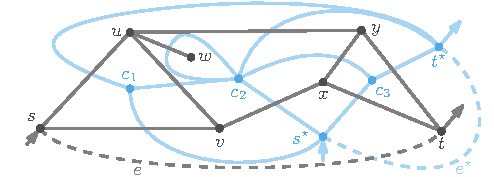
\includegraphics{networkAnalyzes/figures/Dual-Graph.pdf}
    % 
    \caption[Combinatorial dual graphs.]{A plane single-source~\source and
    single-sink~\sink graph~\textcolor{PRIMALGRAPH}{\glssymbol{graph}}
    (\textcolor{PRIMALGRAPH}{dark gray vertices~\tikzStandardVertex} and edges)
    and its combinatorial dual
    graph~\textcolor{DUALGRAPH}{\glssymbol{dualgraph}}
    (\textcolor{DUALGRAPH}{cyan blue vertices~\tikzStandardVertexDual} and
    edges). Adding the~\textcolor{PRIMALGRAPH}{edge~\edge}
    (\textcolor{PRIMALGRAPH}{dark gray dashed line}) divides the outer face into
    two faces representing the faces that include the dual
    source~$\textcolor{DUALGRAPH}{\source^\star}$ and dual
    sink~$\textcolor{DUALGRAPH}{\sink^\star}$ of the~\textcolor{DUALGRAPH}{dual
    graph}. Note that since we have a one-to-one correspondence of the edges,
    adding the edge~\textcolor{PRIMALGRAPH}{\edge} in~\textcolor{PRIMALGRAPH}
    {\glssymbol{graph}} is symmetrical to adding the
    edge~$\textcolor{DUALGRAPH}{\edge^\star}$
    in~\textcolor{DUALGRAPH}{\glssymbol{dualgraph}}.}
    % 
    \label{ch:network-analyzes:sec:mathematical-model:fig:graph-and-the-dual}
    % 
\end{figure}
% 
\textcite[p.13]{Cai12} mention that power grids are planar. A graph is
called~\emph{planar} if it can be embedded into the plane without any edge
crossings, \ie, the edges have no common point, but the two vertices
representing the endpoints of an edge. However, note that there is usually more
than one embedding for a graph~\glssymbol{graph} that is planar. Thus, let us
assume a fixed~\emph{planar embedding}~\glssymbol{embedding} of a
graph~\glssymbol{graph} into the plane
with~$\glssymbol{graph}(\glssymbol{embedding})\cong\glssymbol{graph}$ (\ie,
$\glssymbol{graph}(\glssymbol{embedding})$ is isomorphic to~\glssymbol{graph})
and an injective
function~$\embeddingMap\colon\glssymbol{vertices}\to\reals\times\reals$ meaning
there is a correspondence between the vertices~\glssymbol{vertices} of the graph
and the geometrical points~$\points$ of the plane embedding. An edge
set~$\glssymbol{edges}(\glssymbol{graph})$ of~$\glssymbol{graph}(\embedding)$ is
a subset of a topological space~$\mathcal{T}$, where each edge
in~$\glssymbol{graph}(\embedding)$ is a Jordan curve in~$\mathcal{T}$ and the
incidences and adjacencies are defined accordingly~\parencite{Gro01}.

For power grids such an embedding is usually given by the geographical location
of the network components, where~$\points$ represents the locations of the buses
in terms of latitude and longitude. In addition, we assume a
network~\dcnetworktuple with~$\fmagnitude{\glssymbol{generators}} = 1$
and~$\fmagnitude{\glssymbol{consumers}} = 1$. The vertices that represent the
single generator and single demand are denoted by source~\source and sink~\sink,
respectively.

For plane graphs, we have the concept of duality, which we will link with the
results of duality given
in~\cref{ch:network-analyzes:sec:mathematical-model:subsec:matroids-independence-systems}.
The geometric dual of a plane~\emph{primal graph}~\glssymbol{graph} is called
the~\emph{dual graph}~\glssymbol{dualgraph}. An example is given
in~\cref{ch:network-analyzes:sec:mathematical-model:fig:graph-and-the-dual}. To
construct a dual graph, we introduce the concept of a \emph{face}. We denote
faces by~\face. An \emph{inner face} is a region that is bounded by edges and
vertices in graph~\glssymbol{graph}. We say that these edges are incident to the
face.
% 
The \emph{outer face} is the unbounded region
(see~\cref{ch:network-analyzes:sec:mathematical-model:fig:graph-and-the-dual}
face~$\cycle_\sink$). The dual graph~\glssymbol{dualgraph} is constructed by
introducing a vertex for each face and connecting two vertices if the faces have
an edge in common. Note that we introduce an edge in the dual
graph~\glssymbol{dualgraph} for each edge in the primal graph~\gls{graph}.
% 
% Note that edges where both sides are incident to the same face introduce
% self-loops to the graph
% (see~\cref{ch:network-analyzes:sec:mathematical-model:fig:graph-and-the-dual}
% face~$\cycle_2$ and edge~$\{\vertexa,\vertexc\}$). 
% 
% Note that a self-loop shows that a face represents more than a cycle. However,
% in most cases we can simply
% apply~\cref{ch:network-analyzes:sec:mathematical-model:sim:loop_contraction} to
% reduce the graph. 
Note that a face might represent more than just a cycle, \eg, if
vertex~$\vertexc$
in~\cref{ch:network-analyzes:sec:mathematical-model:fig:graph-and-the-dual} is a
graph itself.
%
%%%%%%%%%%%%%%%%%%%%%%%%%%%%%%%%%%%%%%%%%%%%%%%%%%%%%%%%%%%%%%%%%%%%%%%%%%%%%%%% 
\subsection{Matroids and Independence Systems}
\label{ch:network-analyzes:sec:mathematical-model:subsec:matroids-independence-systems}
%%%%%%%%%%%%%%%%%%%%%%%%%%%%%%%%%%%%%%%%%%%%%%%%%%%%%%%%%%%%%%%%%%%%%%%%%%%%%%%%
% 
% The first two Kirchhoff's laws
% in~\cref{ch:network-analyzes:sec:mathematical-model:eq:kcl-matrix-writing,ch:network-analyzes:sec:mathematical-model:eq:kvl-matrix-writing},
% respectively, focus on the network topology only and do not consider any
% individual behavior of the electrical components (modeled on an edge) such as
% resistors.
% % 
% To cover the electrical components, the third Kirchhoff's law~
% \parencite{Kir47}\parencite[p. 127]{Ses61}
% incorporates these components in a more general sense. However, the third law is
% not relevant to this work and therefore not described formally here. The three
% laws describe the independence of the topology (\ie, \gls{kcl} and~\gls{kvl})
% and the network components (see~\textcite{Kir47}).
% 
% 
A lot of model transformations, properties, and relationships that we use in the
following with regard to matroids (see the postulates of~\textcite[p.510;
Theorem 1]{Whi35}) are based on the discussion by~\textcite{Ses61}
and~\textcite{Whi35,Whi31}. A matroid~\parencite{Whi35} represents a
generalization of a graph~\parencite{Whi31}.
% 
A \emph{matroid} is an abstraction of the independence term that is used in
different fields such as graph theory and geometry. Though different matroids
are considered in different fields, the consensus stays the same. We recall the
definition of a \emph{matroid} by~\textcite[pp.279]{Kor00} (first version was
given by~\textcite[p.510]{Whi35}). A \emph{matroid} is an ordered
pair~$(U,\mathcal{I})$, where~$U$ is the universe
and~$\mathcal{I}\subseteq\mathcal{P}(U)$ is an \emph{independence system}, which
satisfies the following three axioms.
% 
\begin{enumerate}[\textbf{Axiom}~1.]%
    \item $\emptyset\in\mathcal{I}$ (neutral element).
    \label{ch:network-analyzes:sec:mathematical-model:matroid:1}
    % 
    \item If $I\in\mathcal{I}$ and~$I'\subseteq I$ then~$I'\in\mathcal{I}$ 
    (monotonicity).%reflexivity 
    \label{ch:network-analyzes:sec:mathematical-model:matroid:2}
    % 
    \item If~$I_1, I_2\in\mathcal{I}$ with~$\fmagnitude{I_1} < \fmagnitude{I_2}$
    % and~$I_1\cap I_2\not=\emptyset$ 
    then there is an~$e\in (I_2\setminus I_1)$ such
    that~$I_1\cup\{e\}\in\mathcal{I}$ (augmentation).%transitivity
    % 
    \label{ch:network-analyzes:sec:mathematical-model:matroid:3}
\end{enumerate}
% 
Note that the Axiom~\ref{ch:network-analyzes:sec:mathematical-model:matroid:1}
and Axiom~\ref{ch:network-analyzes:sec:mathematical-model:matroid:2} represent
axioms that also hold for any independence system. However, the
Axiom~\ref{ch:network-analyzes:sec:mathematical-model:matroid:3} makes it a
matroid that is a generalization of the term linear independence.
% 
\textcite{Whi35} defines a~\emph{base} as a maximal independent submatroid and
a \emph{cycle} as a minimal dependent submatroid. 
%
\begin{definition}[{{\textcite[p.509]{Whi35}}}]
    A subgraph of a graph is independent if it contains no cycles. 
\end{definition}
% 
In this work, we use an important mathematical principle called \emph{duality}.
In different research areas it has different meanings. However, for us it
basically means that if there is a bijection between the edges (\ie, columns)
in~\glssymbol{incidenceMatrix} and the edges in~\glssymbol{cycleMatrix} and for
a submatroid~$\glssymbol{incidenceMatrix}'$ of~\glssymbol{incidenceMatrix} and
the corresponding dual~$\glssymbol{cycleMatrix}'$ in~$\glssymbol{cycleMatrix}$,
we have the relationship~$\rankx{\glssymbol{cycleMatrix}'} = \rankx{
\glssymbol{cycleMatrix}} - \nullityx{\glssymbol{incidenceMatrix}'}$, 
then~\glssymbol{incidenceMatrix} is a dual of~\glssymbol{cycleMatrix}
and~\glssymbol{cycleMatrix} is a dual
of~\glssymbol{incidenceMatrix}~\parencite[pp.521ff.]{Whi35}. The latter is called
\emph{involution} implying that the dual of the dual
of~\glssymbol{incidenceMatrix} is~\glssymbol{incidenceMatrix} itself. Though
\textquote{every matroid has a dual}~\parencite[p.522; Theorem~22]{Whi35} the
concept applies from a graph-theoretical perspective to plane graphs only. Only
plane graphs have a dual graph.

The following theorems state very central results that are used in this work.
% 
\begin{theorem}[{{\textcite[p.527; Theorem 31]{Whi35}}}]
    %
    For any graph~\glssymbol{graph} the matroids corresponding to its incidence
    matrix~\glssymbol{incidenceMatrix} and its circuit
    matrix~\glssymbol{cycleMatrix} are duals.
    %
    \label{ch:network-analyzes:sec:mathematical-model:thm:matrix-and-its-circuit-matrix-are-duals}
    % 
\end{theorem}
% 
For graphs we restricted the duality to plane graphs, since there is only a dual
graph if the primal graph is planar. For matroids this restriction does not hold
and thus, if we do not restrict ourself to the plane (\ie, sphere with
genus~$0$) but other surfaces with genus greater~$0$, we can still embed a
non-planar graph on a more complex surface without any crossing by making use of
the holes. An example is the embedding of the~$K_5$ on a torus (\ie, surface of
genus~$1$). Note that we focus on planar graph and genus~$0$.
% However, we focus on planar graph and genus 0. The primal matroid is
% the base of the incidence matrix and the dual matroid is the base of the circuit
% matrix.
 
The aforementioned duality
(see~\cref{ch:network-analyzes:sec:mathematical-model:thm:matrix-and-its-circuit-matrix-are-duals})
applies to the matroids~\glssymbol{incidenceMatrix} and~\glssymbol{cycleMatrix}.
% Recall that matroids are generalizations of graphs and thus, all results on
% matroids can be applied on graphs, too.
% 
%
The next theorem follows from
Axiom~\ref{ch:network-analyzes:sec:mathematical-model:matroid:2} and the
aforementioned discussion of the incidence matrix.
%
\begin{theorem}[{{\textcite[p.510; Theorem 1]{Whi35}}}]
    A set~$\glssymbol{incidenceMatrix}'\subseteq\glssymbol{incidenceMatrix}$
    is independent if and only if it is contained in a base, or, if and only if
    it contains no cycles.
\label{ch:network-analyzes:sec:mathematical-model:thm:basis-contain-no-cylces}
\end{theorem}
% 
% Recall that we talk about plane graphs and that only plane graphs have duals
% (see~\cref{ch:network-analyzes:sec:mathematical-model:subsec:planar-graphs}).
The next lemma follows
from~\cref{ch:network-analyzes:sec:mathematical-model:thm:matrix-and-its-circuit-matrix-are-duals}
and is illustrated
in~\cref{ch:network-analyzes:sec:mathematical-model:fig:graph-and-the-dual}.
%
\begin{lemma}[{{\textcite[p.85; Corollary 4-24]{Ses61}}}]
    % 
    If~$\glssymbol{graph}_1$ and~$\glssymbol{graph}_2$ are dual graphs, the
    incidence matrix of either
    graph is a circuit matrix of the other (with the proper rank, and each row
    representing a cycle); that is
    $$ \glssymbol{incidenceMatrix}_1 = \glssymbol{cycleMatrix}_2\text{ and }
    \glssymbol{incidenceMatrix}_2 = \glssymbol{cycleMatrix}_1.$$
    % 
    \label{ch:network-analyzes:sec:mathematical-model:cor:incidence-circuit-matrix-duals}
    % 
\end{lemma}
%
The lemma concludes the duality and is extensively used in this chapter
(see~\cref{ch:network-analyzes:sec:algorithm,ch:network-analyzes:simultaneous-flow-representation}).
% 
%
% 
\begin{figure}[t!]
    % 
    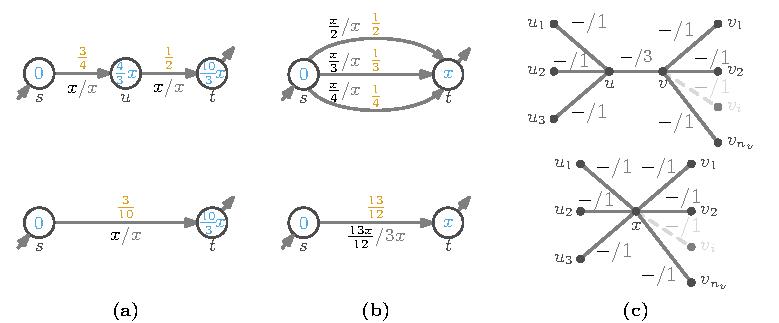
\includegraphics{networkAnalyzes/figures/Series-Parallel-Transformation.pdf}
    % 
    \caption[The series-parallel-contraction and contraction of superfluous
    edges.]{ Three example graphs in which we label each
    vertex~$\vertexa\in\glssymbol{vertices}$ that is represented by a
    cycle~\tikzVertex with a~\textcolor{THETA}{voltage
    angle~$\glssymbol{voltageangle}(\vertexa)$}. If the voltage angles are not
    important, we just use standard bullets~\tikzStandardVertex. On the edges,
    we write the flow~\glssymbol{flow} and the edge's
    capacity~\glssymbol{capacity} in the form~$\glssymbol{flow} /
    \textcolor{CAPACITY}{\glssymbol{capacity}}$. If
    the~\textcolor{SUSCEPTANCE}{susceptance~\glssymbol{susceptance}} is
    important for the transformation, we write it on the edge.

    The series-parallel-contraction and contraction of superfluous edges
    in energy networks simplifies the graph structure. (a) In a
    series-contraction a path is contracted to a single edge. (b) In a
    parallel-contraction multiple parallel edges (multi-edges) are contracted to
    one edge.
    % 
    (c)~A scenario where shortening of superfluous edges
    (\cref{ch:network-analyzes:sec:mathematical-model:sim:edge_shortening}) is
    reasonable. This figure is adapted from~\parencite[p.313; Figure~4]{Ake60}.
    The upper figure is an example, where the capacity of edge~$
    \glssymbol{capacity}(\vertexa,\vertexb)\geq\min\big(\sum_{
    \{\vertexa_i,\vertexa\}\in\glssymbol{edges}}\glssymbol{capacity}(\vertexa_i,\vertexa),\sum_{
    \{\vertexb_i,\vertexb\}\in\glssymbol{edges}}\glssymbol{capacity}(\vertexb_i,\vertexb)\big)$.
    In the bottom figure the resulting graph after contracting the superfluous
    edge~$\{\vertexa,\vertexb\}$
    to a vertex~$x$ is shown. 
    }
    % 
    \label{ch:network-analyzes:sec:mathematical-model:fig:SeriesParallelContraction}
\end{figure}
%
% 
%%%%%%%%%%%%%%%%%%%%%%%%%%%%%%%%%%%%%%%%%%%%%%%%%%%%%%%%%%%%%%%%%%%%%%%%%%%%%%%
\section{Electrical Preserving Transformations}
\label{ch:network-analyzes:sec:reduction-transformation-rules}
%%%%%%%%%%%%%%%%%%%%%%%%%%%%%%%%%%%%%%%%%%%%%%%%%%%%%%%%%%%%%%%%%%%%%%%%%%%%%%%
%
In this section, we introduce some standard reduction rules used in literature
that lead in the end to an algorithm to solve the~\gls{dc}~\gls{feas}. Most
transformations make use of the superposition principle for linear power grids,
\eg, the~\deltawye- and~\wyedelta-transformations. The superposition principle
holds (\ie, used for the superposition of, \eg, forces), since the constraint
matrix~\constraintmatrix is a linear map and thus, superposition becomes a
simple addition of linear equations (\ie, standard operation in a
field~$\mathbb{F}$). Though we give rules to compute the
capacity~\glssymbol{capacity}, these formulas can be dependent on the actual
flow
(see~\cref{ch:network-analyzes:sec:mathematical-model:sim:deltawye_transformation}).
Computing any electrical flow becomes trivial if we contract the graph to one
edge since on trees the electrical flow is equivalent to a graph-theoretical
flow~\parencite{Lei15b}\parencite[p.9; Lemma~4]{Leh15a}.

Recall that we have a unique electrical flow in~\source-\sink-graphs
(see~\cref{ch:network-analyzes:sec:mathematical-model:lem:unique-flow}), we can
scale it to a multiple such that it complies with the capacity constrains
(\cref{ch:network-analyzes:sec:mathematical-model:eq:capacity-constraint}).
Thus, we are able to neglect the capacity constraints and rescale the electrical
flow afterwards such that the capacity constraints are fulfilled
using~\cref{ch:network-analyzes:sec:mathematical-model:lem:rescalling-to-mpf}.
From
the~\cref{ch:network-analyzes:sec:mathematical-model:eq:KCL-intermediate-vertex,ch:network-analyzes:sec:mathematical-model:eq:KCL-generator-vertex,ch:network-analyzes:sec:mathematical-model:eq:KCL-consumer-vertex,ch:network-analyzes:sec:mathematical-model:eq:kvl-ohm-function-writing},
we have only one component that has a crucial influence on the electrical flow
and that is the susceptance~\glssymbol{susceptance}. The susceptance represents
a ratio that can be interpreted as how many electrons go through a path. Thus,
the notion of electrical preserving is purely susceptance based.
% 
\begin{definition}[Electrical Preserving Transformation]
    % 
    Let~\glssymbol{flow} be a given flow and let~$\glssymbol{voltageangle}
    (\vertexa)$ be the voltage angles before the transformation for
    all~$\vertexa\in\glssymbol{vertices}(\glssymbol{graph})$ with regard
    to~\glssymbol{flow}. An electrical preserving transformation~$\mathcal{T}$
    on~\glssymbol{network} is a function~$
    % 
        \mathcal{T}
        \colon 
            % \glssymbol{vertices} 
            % \times
            % \glssymbol{undirectededges}
            \mathcal M (\glssymbol{network})
            % \times
            % \glssymbol{susceptance} 
        \to %\glssymbol{vertices}
            %\times
            %\glssymbol{undirectededges}
            \mathcal M (\glssymbol{network})
            % \times
            % \glssymbol{susceptance}
    % 
    $ with~$
    % 
        (
        \glssymbol{graph} 
        =
        (
        \glssymbol{vertices},
        \glssymbol{undirectededges}
        ),
        \glssymbol{susceptance}
        ) 
        \mapsto 
        (
        \glssymbol{graph}'
        =
        (
            \glssymbol{vertices}',
            \glssymbol{undirectededges}'
        ),
        \glssymbol{susceptance}'
        )
    % 
    $ and new voltage angle assignments~$
        % 
        \glssymbol{voltageangle}'(\vertexa)
        % 
    $ for all~$\vertexa\in\glssymbol{vertices}'$ such that the susceptances are
     transformed in such a way that for the flow~\glssymbol{flow} we have~$
        %
        \glssymbol{voltageangle}'(\vertexa) 
        =
        \glssymbol{voltageangle}(\vertexa)
        % 
    $ for all vertices~$
        % 
        \vertexa
        \in
        (
            \glssymbol{vertices}
            \cap
            \glssymbol{vertices}'
        )
        % 
    $.
    % An electrical preserving transformation results in a susceptance that
    % preserves the initial susceptance ratio for each vertex pair that takes
    % part on the transformation.
    % 
    \label{ch:network-analyzes:sec:mathematical-model:def:electrical-preserving}
\end{definition}
% 
% However, if we have a network with a single generator and a single consumer it
% follows
% from~\cref{ch:network-analyzes:sec:mathematical-model:lem:rescalling-to-mpf}
% that we can neglect the capacities
% (see~\cref{ch:network-analyzes:sec:mathematical-model:eq:capacity-constraint}),
% since the flow can be post scaled and apply any electrical flow. 
% 
Transformation rules are useful to simplify the network and compute network
parameter more efficiently. Examples are the effective values, \eg, effective
resistance, conductance/susceptance, the \textquote{effect of earth admittances
on the balance of a Wheatstone bridge and earth capacity effects
in~\gls{ac}}~\parencite{Ros24,But21}, and the effective unbalanced
capacity~\parencite[p.916]{Ros24}.

For edges that operate in series---meaning they represent a path---where there
is no generator or demand vertex in between, we know that the
flow~$\glssymbol{flow}$ on each edge along the path is the same. Lets assume a
path with two edges~$
    % 
    \{\vertexa,\vertexb\},
    \{\vertexb,\vertexc\}
    \in
    \glssymbol{undirectededges}
    % 
$. Since all mappings are linear and we work on a field~$\mathbb F$
(\ie, here it is~\reals), we get the following relationship~$
    % 
    \nicefrac{
        \big(
            \glssymbol{voltageangledifference}_1(\vertexa,\vertexb)
            + 
            \glssymbol{voltageangledifference}_2(\vertexb,\vertexc)
        \big)
    }{ 
        \glssymbol{flow}
    }
    =
    \nicefrac{1}{ \glssymbol{susceptance}_1(\vertexa,\vertexb) }
    +
    \nicefrac{1}{ \glssymbol{susceptance}_2(\vertexb,\vertexc) }
    =
    \nicefrac{1}{ \glssymbol{susceptance}(\vertexa,\vertexc) }
    % 
$ with~$
    % 
    \glssymbol{flow}(\vertexa,\vertexb) 
    = 
    \glssymbol{flow}(\vertexb,\vertexc) 
    = 
    \glssymbol{flow}
    % 
$, which we will generalize in the following rule.
% 
\begin{reductionrule}[Series Contraction]
    % 
    Let~$\fpath{}{\vertexa}{\vertexc}$ be a simple terminal-free path (\ie, for
    internal vertices of the path holds
    that~$\vertex\in\glssymbol{vertices}\setminus\big
    (\{\vertexa,\vertexc\}\cup\glssymbol{generators}\cup\glssymbol{consumers}\big)$)
    whose internal vertices~$\vertex\in\fpath{}{\vertexa}{\vertexc}$ with
    $\vertex\not=\vertexa,\vertexc$ have degree~$\degree(\vertex) = 2$. Then, 
    such a path~$\fpath{}{\source}{\sink}\coloneqq\big( (\source,\vertexa_1),
    (\vertexa_1,\vertexa_2),\dots, (\vertexa_i,\sink) \big)$ is equivalent to
    one
    edge~$(\source,\sink)$~(see~\cref{ch:network-analyzes:sec:mathematical-model:fig:SeriesParallelContraction}\screen{a})
    with the susceptance, voltage angle difference, and capacity being 
    % 
    \begin{subequations}
    \begin{align}
        \glssymbol{susceptance}(\vertexa,\vertexc) 
        &= 
        {\left(\sum_{\edge\in\fpath{}{\vertexa}{\vertexc}}\glssymbol{susceptance}(\edge)^
        {-1}\right)}^{-1},\\
        % 
        \glssymbol{voltageangledifference}(\vertexa,\vertexc)
        &= \frac{\min_{\edge\in\glssymbol{path}(\vertexa,\vertexc)}\glssymbol{capacity}
        (\edge)}
        {\glssymbol{susceptance}(\vertexa,\vertexc)},\\
        % 
        \glssymbol{capacity}(\vertexa,\vertexc)
        &=
        \glssymbol{susceptance}(\vertexa,\vertexc) 
        \cdot
        \glssymbol{voltageangledifference}(\vertexa,\vertexc),
    \end{align}
    \end{subequations}
    % 
    respectively.
    % 
    \label{ch:network-analyzes:sec:mathematical-model:sim:series_contraction}
    % 
\end{reductionrule}
% 
For multiple parallel edges between two vertices~$\vertexa, \vertexb \in 
\glssymbol{vertices}(\glssymbol{graph})$, we can make the observation that the
voltage
angles~$
    \glssymbol{voltageangle}(\vertexa)
$ and
$
    \glssymbol{voltageangle}(\vertexb)
$ are the same for each edge. Thus, the voltage angle difference~$
    % 
    \glssymbol{voltageangledifference}(\vertexa,\vertexb)
    % 
$ is the same. Since we work on a field~$\mathbb{F}$ and have linear maps only,
we do a simple addition operation on a field such that we get~$
    % 
    \nicefrac{
        \big(
        \glssymbol{flow}\left( \{\vertexa,\vertexb\}^1 \right) 
        + 
        \glssymbol{flow}\left( \{\vertexa,\vertexb\}^2 \right)
        \big)
    }{
        \glssymbol{voltageangledifference}(\vertexa,\vertexb)
    } 
    % 
    = 
    % 
    \glssymbol{susceptance}(\{\vertexa,\vertexb\}^1) 
    +
    \glssymbol{susceptance}(\{\vertexa,\vertexb\}^2)
    =
    \glssymbol{susceptance}(\vertexa,\vertexb)
    % 
$ for two parallel edges~$
    % 
    \{\vertexa,\vertexb\}^1, 
    \{\vertexa,\vertexb\}^2
    \in 
    \glssymbol{undirectededges}
    % 
$. We generalize this to multiple edges in the following rule.
% 
\begin{reductionrule}[Parallel Contraction]
    Let~$
        p
        \colon
        \glssymbol{undirectededges}
        \to
        \{
            \{\vertexa,\vertexb\}
            \mid
            \vertexa,
            \vertexb
            \in
            \glssymbol{vertices};
            \vertexa
            \not\eq
            \vertexb
        \}
    % 
    $ with~$
        % 
        % \left\{ 
        \{\vertexa,\vertexb\}^i
        % \right\}
        \mapsto 
        \{\vertexa,\vertexb\} 
        % 
    $ with~$1\leq i\leq k$ being~$k$ parallel edges. Let the parallel edges be~$
        % 
        \edge_i
        \colon
        \{\vertexa,
        \vertexb\}^i
        \in
        \glssymbol{undirectededges}
        % 
    $ with~$1\leq i\leq k$, \ie, $p(\edge_i) = p(\edge_{i+1})$ for all~$1\leq
    i\leq k-1$. These parallel edges are equivalent to one
    edge~(see~\cref{ch:network-analyzes:sec:mathematical-model:fig:SeriesParallelContraction}\screen{b})
    with the susceptance~\glssymbol{susceptance}, voltage angle
    difference~\glssymbol{voltageangledifference}, and
    capacity~\glssymbol{capacity} being
    % 
    \begin{subequations}
    \begin{align}
        % 
        \glssymbol{susceptance}(\vertexa,\vertexb) 
        &= 
        \sum_{
            \{\vertexa,\vertexb\}^i
            \in
            \glssymbol{undirectededges}
        }
        \glssymbol{susceptance}
        \left(
            \{\vertexa,\vertexb\}^i
        \right),
        % 
        \\%
        % 
        \glssymbol{voltageangledifference}(\vertexa,\vertexb)
        ~&=~ 
        \min_{
            \{\vertexa,\vertexb\}^i
            \in
            \glssymbol{undirectededges}
        } 
        \left(
            \glssymbol{voltageangledifference}
            \left(
                \left\{
                    \vertexa,\vertexb
                \right\}^i
            \right)
        \right),
        % 
        \\%
        % 
        \fcapacity{}{\vertexa}{\vertexb}
        &=
        \glssymbol{susceptance}(\vertexa,\vertexb) 
        \cdot
        \glssymbol{voltageangledifference}(\vertexa,\vertexb),
        % 
    \end{align}
    \end{subequations}
    % 
    respectively.
    % 
    \label{ch:network-analyzes:sec:mathematical-model:sim:parallel_contraction}
    % 
\end{reductionrule}%
% 
Every vertex~$\vertex\in\glssymbol{vertices}$ has a voltage
angle~$\glssymbol{voltageangle}(\vertex)$ that can be interpreted as a
potential. For a self-loop the voltage angles at both ends are the same and
thus, the flow~\glssymbol{flow} on the self-loop is zero
(see~\cref{ch:network-analyzes:sec:mathematical-model:eq:kvl-ohm-function-writing}).
% 
\begin{reductionrule}[Self-loop Contraction]%
    % 
    Let~$
        % 
        p
        \colon
        \glssymbol{undirectededges}
        \to
        \{
            \{\vertexa,\vertexb\}
            \mid
            \vertexa,
            \vertexb
            \in
            \glssymbol{vertices}
            % ;
            % \vertexa = \vertexb
        \}
        % 
    $
    be a function with~$
        % 
        \{\vertexa,\vertexa\} 
        \mapsto
        \{\vertexa\}
        % 
    $, where~$p(\edge)=
    \{\vertexa\}$ with~$\edge\in\glssymbol{undirectededges}$ is
    a self-loop with both ends of edge~\edge ending in~\vertexa. Then the
    edge~\edge can be removed without any electrical effect, but with one edge
    less
    (see~\cref{ch:network-analyzes:sec:mathematical-model:eq:kvl-ohm-function-writing}
    with the additional note that both voltage angles are the same and thus, the
    difference is zero).
    % 
    \label{ch:network-analyzes:sec:mathematical-model:sim:loop_contraction}
    % 
\end{reductionrule}%
% 
\begin{reductionrule}[Degree-1 Contraction]%
    % 
    Let~$
        % 
        \vertexa
        \in
        \glssymbol{vertices}
        \setminus
        (\glssymbol{generators}\cup\glssymbol{consumers})
        % 
    $ be a vertex with degree~$\degree(\vertexa) = 1$ with its only edge~$
    (\vertexa,\vertexb)$. Then~\vertexa can be removed.
    % 
    \label{ch:network-analyzes:sec:mathematical-model:sim:degree_1_contraction}%
    % 
\end{reductionrule}%
% 
% If the edge~$%
%     % 
%     \{\vertexa,\vertexb\}\in\glssymbol{undirectededges}%
%     % 
% $ of the degree-$1$ vertex~\vertexa is superfluous in the sense that $
%     %
%     \sum_{
%         \{\vertexb,\vertexc\}
%         \in
%         \glssymbol{undirectededges}
%         \setminus
%         \{\{\vertexa,\vertexb\}\} 
%     }
%     \glssymbol{capacity}(\vertexb,\vertexc)
%     \leq
%     \glssymbol{capacity}(\vertexa,\vertexb)
%     % 
% $ then~$\vertexa\in\glssymbol{vertices}$ suffices (meaning that it can be also a
% generator or consumer).
% 
The next reduction rule can be used for shortest paths and graph-theoretical
flows. However, in general it is not applicable for electrical networks. We
remark that in the next section we only work with shortest paths and
graph-theoretical flows.
%
\begin{reductionrule}[Shortening of Superfluous Edges~{{\parencite[p. 313; Rule 3]
{Ake60}}}]
    % 
    Let~$\vertexa\in\glssymbol{vertices}$ and let~$
    \{\vertexa,\vertexc\}\in\glssymbol{undirectededges}$ be an incident
    edge with capacity~$$
        \fcapacity{}{\vertexa}{\vertexc}
        \geq
        \min
        \left(
            \sum_{
                \{\vertexa,\vertexb\}
                \in
                \glssymbol{undirectededges}
                \setminus
                \{
                    \{\vertexa,\vertexc\}
                \}
            }
            \fcapacity{}{\vertexa}{\vertexb}, 
            \sum_{
                \{\vertexc,\vertexb\}
                \in
                \glssymbol{undirectededges}
                \setminus
                \{
                    \{\vertexa,\vertexc\}
                \}
            }
            \fcapacity{}{\vertexc}{\vertexb}
        \right)$$
    (see~\cref{ch:network-analyzes:sec:mathematical-model:fig:SeriesParallelContraction}\screen{c}
    top) then we can contract vertices~\vertexa and~\vertexb to a new
    vertex~$x$
    (see~\cref{ch:network-analyzes:sec:mathematical-model:fig:SeriesParallelContraction}\screen{c}
    bottom).
    % 
    \label{ch:network-analyzes:sec:mathematical-model:sim:edge_shortening}
    % 
\end{reductionrule}
% 
A more general example of the latter transformation is applied on~\parencite[p.
316; Figure 7]{Ake60} in the third transformation.

% 
\begin{figure}[t!]
    % 
    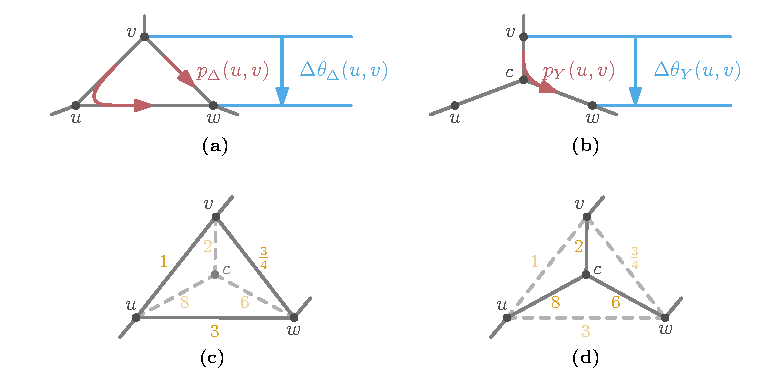
\includegraphics{networkAnalyzes/figures/Delta-Wye-Transformation.pdf}
    % 
    \caption[The delta-wye- and wye-delta-transformations.]{The delta-wye-
    (\cref{ch:network-analyzes:sec:mathematical-model:sim:deltawye_transformation})
    and wye-delta-transformations
    (\cref{ch:network-analyzes:sec:mathematical-model:sim:wyedelta_transformation})
    represent possible transformation rules in electrical networks. In this
    example, we have a graph with three (respectively four)
    vertices~\tikzStandardVertex. If we explicitly compute the susceptances we
    write the \textcolor{SUSCEPTANCE}{susceptance~\glssymbol{susceptance}} on
    each edge. (a)~The triangle~$\Delta$ can be transformed to a star~$Y$.
    Recall that we have only linear maps and work on a field~$\mathbb F$
    (here~\reals). Thus, we can superpose the paths that is a simple addition
    operation, \eg, $ (\vertexb,\vertexc)$ is equal to the series circuit
    of~$(\vertexb,\vertexa)$ and~$(\vertexa,\vertexc)$, which is parallel
    to~$(\vertexb,\vertexc)$ meaning~$
        % 
        \big(
            (\vertexb,\vertexa),
            (\vertexa,\vertexc)
        \big)
        ||
        (\vertexb,\vertexc)
        % 
    $.
    This electrical addition can be done for the \textcolor{SUSCEPTANCE}
    {susceptances~\glssymbol{susceptance}} and \textcolor{KITred70}{electrical
    (\eg, power) flows~$\glssymbol{realpower}$}. The voltage angle (potential)
    difference stays the same~$
        % 
        \textcolor{THETA}{\glssymbol{voltageangledifference}}
        % 
    $. (b)~This star~$Y$ can be transformed to a triangle~$\Delta$ and can use
    similar properties as described in~\mbox{(a)}.
    (c)~The~\deltawye-transformation increases the number of vertices by one and
    decreases the number of cycles by one. (d)~The~\wyedelta-transformation
    increases the number of cycles by one and decreases the number of vertices
    by one.}
    % 
    \label{ch:network-analyzes:sec:mathematical-model:fig:DeltaWyeTransformation}
    % 
\end{figure}
% 
The next graph transformations are more complex and were first introduced
by~\textcite{Ken99}. The~\deltawye-Transformation (also known as Delta-Wye- or
Triangle-Star-Transformation) and~\wyedelta-Transformation are inversions to
each other.
% 
\begin{reductionrule}[\deltawye-Transformation]
    % 
    Let~\vertexa, \vertexb, and~\vertexc form a complete graph with the edge
    set~$\glssymbol{undirectededges}_{\Delta}\subseteq\glssymbol{undirectededges}$
    (see~\cref{ch:network-analyzes:sec:mathematical-model:fig:DeltaWyeTransformation}\screen{a}).
    This delta~$\Delta$ can be transformed to a wye~$Y$ by adding a new
    vertex~\vertexStar representing the center of the wye~$Y$
    to~$\glssymbol{vertices}$ and new edges to the triangle's vertices~$
        % 
        \glssymbol{undirectededges}
        \cup
        \big\{
            \{\vertexStar,\vertexa\}
            \mid
            \{\vertexa,\vertexb\}
            \in
            \glssymbol{undirectededges}_{\Delta}
        \big\}
        \setminus
        \glssymbol{undirectededges}_{\Delta}
        % 
    $
    (see~\cref{ch:network-analyzes:sec:mathematical-model:fig:DeltaWyeTransformation}\screen{b}).
    % 
    \begin{subequations}
        \begin{align}
        %
        \glssymbol{susceptance}(\vertexa,\vertexStar)%
        &= 
        \frac{
            \glssymbol{susceptance}(\vertexa,\vertexb)%
            \cdot
            \glssymbol{susceptance}(\vertexa,\vertexc)%
            +
            \glssymbol{susceptance}(\vertexa,\vertexb)%
            \cdot
            \glssymbol{susceptance}(\vertexb,\vertexc)%
            +
            \glssymbol{susceptance}(\vertexa,\vertexc)%
            \cdot
            \glssymbol{susceptance}(\vertexb,\vertexc)%
        }{
            \glssymbol{susceptance}(\vertexb,\vertexc)%
        }\\%
        %
        \glssymbol{capacity}(\vertexa, \vertexStar) 
        &= 
        \glssymbol{capacity}(\vertexa,\vertexb) 
        + 
        \glssymbol{capacity}(\vertexa,\vertexc) 
        - 
        \big(%
            \glssymbol{flow}(\vertexb,\vertexStar)%
            -%
            \glssymbol{flow}(\vertexc, \vertexStar)%
        \big)%
        %
        \end{align}
    \end{subequations}
    % 
    \label{ch:network-analyzes:sec:mathematical-model:sim:deltawye_transformation}%
    % 
\end{reductionrule}
% 
The inverse rule of the~\deltawye-transformation is denoted
by~\wyedelta-Transformation.
% 
\begin{reductionrule}[\wyedelta-Transformation]
    Let~$
        % 
        \vertexStar
        \in
        \glssymbol{vertices}
        \setminus
        (\glssymbol{generators}\cup\glssymbol{consumers})
        % 
    $ be a vertex with a degree of~$\degree(\vertexStar) = 3$
    (see~\cref{ch:network-analyzes:sec:mathematical-model:fig:DeltaWyeTransformation}\screen{b}
    and~\screen{d}). Thus, vertex~\vertexStar forms the center of a wye~$Y$ with
    neighbors~\vertexa, \vertexb, and~\vertexc. The transformation of the
    wye~$Y$ results in a equivalent network that is a delta~$\Delta$ by~$
        % 
        \glssymbol{undirectededges}''
        \cup
        \big\{
            \{\vertexa,\vertexb\}
            \mid
            \{\vertexStar,\vertexa\}
            \in
            \glssymbol{undirectededges},
            \{\vertexStar,\vertexb\}
            \in
            \glssymbol{undirectededges}~\text{with}~\vertexa
            \not\eq
            \vertexb
        \big\}
        \setminus
        \big\{
            \{\vertexStar,\vertexa\}
            \in
            \glssymbol{undirectededges}
        \big\}
        % 
    $ and~$
        % 
        \glssymbol{vertices}
        \setminus
        \{\vertexStar\}
        % 
    $
    (see~\cref{ch:network-analyzes:sec:mathematical-model:fig:DeltaWyeTransformation}%
    \screen{a} and~\screen{c}) with the susceptances
    % 
    \begin{align}
        % 
        \glssymbol{susceptance}(\vertexa,\vertexb) 
        &= 
        \frac{
            \glssymbol{susceptance}(\vertexa,\vertexStar)
            \cdot
            \glssymbol{susceptance}(\vertexb,\vertexStar)
        }{
            \glssymbol{susceptance}(\vertexa,\vertexStar) 
            + 
            \glssymbol{susceptance}(\vertexb,\vertexStar) 
            + 
            \glssymbol{susceptance}(\vertexc,\vertexStar)
        }.
        % 
    \end{align}
    % 
    \label{ch:network-analyzes:sec:mathematical-model:sim:wyedelta_transformation}
    % \franzi{How to transform the capacity?}
\end{reductionrule}
% 
The basic idea of the latter transformation is that we remove a
vertex~\vertexStar that is the center of a wye~$Y$ and connect all its neighbors
by an edge. Note that the previous transformation removes a vertex from the
graph, which reduces the size of the network. The next transformation is a
generalization
of~\cref{ch:network-analyzes:sec:mathematical-model:sim:wyedelta_transformation}.

Note that a star of arbitrary degree~$\deg(\vertexStar)$, where~\vertexStar is
the center of a star, is a more general notation for wye and in this case a
\emph{polygon} is a complete graph~$K_{\deg(\vertexStar)}$ representing a
generalization of a triangle (\ie, $K_3$).
% 
% TODO: N(c) independent?
%  
\begin{reductionrule}[Star-Polygon-Transformation~{{\parencite[p.916]{Ros24}}}]
    % 
    Let~$\vertexStar\in\glssymbol{vertices}\setminus(\glssymbol{generators}\cup
    \glssymbol{consumers})$ be a vertex with a degree of~$\degree(\vertexStar)$.
    Thus, vertex~\vertexStar forms the center of a star with
    neighbors~$\neighbor(\vertexStar)$. Transforming a star into a polygon
    by~$
        % 
        \glssymbol{edges}'
        =
        \glssymbol{edges}
        \cup
        \big\{
            \{\vertexa,\vertexb\}
            \mid
            \vertexa 
            \in
            \neighbor(\vertexStar), 
            \vertexb 
            \in
            \neighbor(\vertexStar)~\text{with}~\vertexa
            \not\eq
            \vertexb
        \big\}
        \setminus
        \big\{
            \{\vertexStar,\vertexa\}
            \in
            \glssymbol{edges}
            \mid
            % \forall
            \vertexa
            \in
            \neighbor(\vertexStar)
        \big\}
        % 
    $
    and~$
        % 
        \glssymbol{vertices}' 
        = 
        \glssymbol{vertices}
        \setminus
        \{\vertexStar\}
        % 
    $, we get the susceptances
    % 
    \begin{align}
        \glssymbol{susceptance}(\vertexa,\vertexb) 
        &= 
        \frac{
        \glssymbol{susceptance}(\vertexa,\vertexStar)
        \cdot
        \glssymbol{susceptance}(\vertexb,\vertexStar)
        }{
            \sum_{
                \{\vertexa,\vertexStar\}
                \in
                \glssymbol{edges}
            }
            \glssymbol{susceptance}(\vertexa,\vertexStar)
        }
        \qquad
        \forall
        \vertexa,\vertexb
        \in
        \neighbor(\vertexStar).%
    \end{align}
    % 
    % the transformation has no general inverse without additional constraints
    % - by polygon they mean a complete graph
    % \franzi{Check: \parencite{Lie73,Bed61,CURTIS1998115}}
    % \cite{shew1947xxvii} inverse transformation under Wheatstone's condition
    \label{ch:network-analyzes:sec:mathematical-model:sim:star-polygon-transformation}
\end{reductionrule}
% 
One of the first applications is given by~\textcite{But21} on the earth capacity
effects. \textcite[p.917; Figure 3]{Ros24} calculates the effective conductance
between two terminals using the next transformation. \textcite[p.917; Figure
4]{Ros24} calculates the effect on the balance of Wheatstone bridges by the
earth admittance between two terminals using the latter transformation.% Similar
% results exist for double-bridge networks and Wagner double bridge/Wien
% bridges~\franzi{?}.

Note that if there is already an
edge~$\{\vertexa,\vertexb\}\in\glssymbol{undirectededges}$, we can apply in
addition
to~\cref{ch:network-analyzes:sec:mathematical-model:sim:star-polygon-transformation}
a parallel contraction in form
of~\cref{ch:network-analyzes:sec:mathematical-model:sim:parallel_contraction}.
We now reference two other reduction rules for the sake of completeness.
%
\begin{reductionrule}[Polygon-to-Chain-Reduction~{{\parencite{Sat85}}}]
    % 
    See~\textcite{Sat85} for more information.
    % 
    \label{ch:network-analyzes:sec:mathematical-model:sim:polygon_to_chain_reduction}
    % 
\end{reductionrule}
% 
% - \textcite{1086780} formulated an open question 
% - one \textcite{Bed61} provided a necessary relationship that takes
% the product of the admittances of the two parallel branches and equating it with
% the product of the admittances of the two diagonal branches of the
% quadrilateral
% -> sufficiency requires that every one in th edet satisfy the condition

% - Idea: Basically checks symmetry required by \textcite[p.916;(1)]{Ros24}
%
\begin{reductionrule}[Trisubgraph-Y-Reduction~{{\parencite{Sat93}}}]
    % 
    See~\textcite{Sat93} for more information.
    % 
    \label{ch:network-analyzes:sec:mathematical-model:sim:polygon_to_chain_reduction}
    % 
\end{reductionrule}
% 
We denote a graph~\glssymbol{graph} to be \emph{$k$-edge reducible} if there is
a series of application of reduction rules 
(\cref{ch:network-analyzes:sec:mathematical-model:sim:series_contraction,ch:network-analyzes:sec:mathematical-model:sim:parallel_contraction,ch:network-analyzes:sec:mathematical-model:sim:deltawye_transformation,ch:network-analyzes:sec:mathematical-model:sim:wyedelta_transformation})
such that the resulting graph has only~$k$ remaining edges.
% 
\begin{theorem}[{{\textcite{Epi66}}}]
    % 
    Every biconnected plane \source-\sink-graph with an~$(\source,\sink)$-edge
    is $1$-edge reducible.
    % 
    \label{ch:network-analyzes:sec:mathematical-model:thm:epifanov}
    % 
\end{theorem}
%
\begin{wrapfigure}{l}{4.5cm}%
    % 
    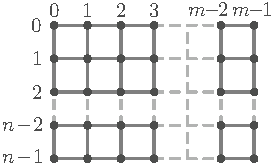
\includegraphics[scale=1,page=1]{networkAnalyzes/figures/GridGraph.pdf}
    % 
    \caption[A grid graph.]{%
    % 
    A grid graph~\glssymbol{graph} of size~$n\times m$ with~$n, m \geq 2$.
    %
    }%
    % 
    \label{ch:network-analysis:fig:grid-graph}%
    % 
\end{wrapfigure}% 
% 
\noindent To understand the next result, we define grid graphs and minors. A
(square)~\emph{grid graph}~$
    % 
    \glssymbol{graph}_{\mathrm{grid}} 
    = 
    (
    \glssymbol{vertices}_{\mathrm{grid}},
    \glssymbol{edges}_{\mathrm{grid}}
    )
    % 
$ (also known as lattice graph) is a plane graph, where each edge has unit
length and is drawn either by a horizontal or a vertical straight curve. The
grid points are crossings represented by vertices
(\cref{ch:network-analysis:fig:grid-graph}). A~\emph{minor} is a graph that can
be obtained from a graph~\glssymbol{graph} by contracting edges and by deleting
vertices and edges.

\noindent We use the following results to provide a first algorithm
for~\gls{dc}~\gls{feas} and~\gls{mpfp} on
plane~\source-\sink-graphs~\glssymbol{graph}.
%%%%%%%%%%%%%%%%%%%%%%%%%%%%%%%%%% ALGORITHM %%%%%%%%%%%%%%%%%%%%%%%%%%%%%%%%%%%
%
% \wormhole{bit:ch:switching:sec:exploit_structural_characteristics:subsec:dtp:alg:shortest_theta_path}
% \def\HiLi{\leavevmode\rlap{\hbox to \hsize{\color{HiLi}\leaders\hrule
% height .9\baselineskip depth 1.3ex\hfill}}}
\begin{algorithm}[tb!]%
\SetAlgoLined
%%%%%%%%%%%%%%%%%%%%%%%%%%%%%%%%%%
% 
\KwData{A network~\dcnetworktuple with~$\fmagnitude{\glssymbol{generators}} = 1$ (\ie,
$\{\source\} = \glssymbol{generators}$), $\fmagnitude{\glssymbol{consumers}} = 1$ 
(\ie, $\{\sink\} = \glssymbol{consumers}$), 
$\realpowergeneration = \realpowergenerationmin = \realpowergenerationmax$, 
and $\realpowerdemand = \realpowerdemandmin = \realpowerdemandmax$.}
% 
\KwResult{Flow~$\glssymbol{flow}(\vertexa,\vertexc)$ for all $
(\vertexa,\vertexc)\in\glssymbol{edges}$, flow value~$\glssymbol{flowvalue}(\glssymbol{flow},\glssymbol{network})$, and
voltage angles~$\glssymbol{voltageangle} (\vertexa)$
with~$\vertexa\in\glssymbol{vertices}$.}
% 
% INITIALIZATION %%%%%%%%%%%%%%%%%%%%%%%%%%%%%%%%%%%%%%%%%%%%%%%%%%%%%%%%%%%%
% 
$\embedding\hspace{4mm} = \algoplanarembedding(\glssymbol{graph})$
\hspace*{-1mm}%
\label{ch:network-analyzes:algo:stpf:planarEmbedding}
\Comment*{\color{KITblack30} PQ-Tree; see~\cref{ch:network-analyzes:sec:planar-embedding-dual-graph-construction}}%
% 
$\embedding_{\mathrm{grid}} 
= 
\algoGridEmbeddingOfPlanarGraph(\glssymbol{graph}(\embedding))$
\label{ch:network-analyzes:algo:stpf:gridEmbedding}
\Comment*{\color{KITblack30} see~\cref{ch:network-analyzes:sec:mathematical-model:lemma:embedding-into-a grid}}%
% 
$
\big( 
    \gls{network} = \gls{network}_0
    ,\dots
    ,\gls{network}_k 
        = \big( 
            (\{\source,\sink\}, \{\edge'\})
            , \{\source\}
            , \{\sink\}
            ,\gls{capacity}'
            ,\gls{susceptance}'
            ,\realpowergeneration
            ,\realpowerdemand) 
          \big)
\big) \allowbreak
\hspace*{5mm}= 
\algoContractGridGraphToEdge(\gls{network}(\embedding_{\mathrm{grid}}))$
\label{ch:network-analyzes:algo:stpf:contractGridGraphToEdge}%
\Comment*{\color{KITblack30} see~\cref{ch:network-analyzes:sec:mathematical-model:lem:grid-graph-deltawye-reducible}}%
$\gls{flow}(\edge') = \realpowergeneration = \realpowerdemand$
\label{ch:network-analyzes:algo:stpf:flowAssignment}%
\;
% 
$
    \glssymbol{flow}
    \hspace{5mm}=
    \algoDecontractEdgeToGridGraph((\gls{network}_0,\dots,\gls{network}_k),\flow(\edge'))
$
\label{ch:network-analyzes:algo:stpf:decontractGridGraphToEdge}%
\;
% 
$
    \gls{flow} 
    \hspace{5mm}= 
    \algoRescalePowerFlow(\gls{network},\gls{flow})$%
\label{ch:network-analyzes:algo:stpf:rescaling}%
\Comment*{\color{KITblack30} see~\cref{ch:network-analyzes:sec:mathematical-model:lem:rescalling-an-pf}}%
% 
\Return~\glssymbol{flow}\;
%
%%%%%%%%%%%%%%%%%%%%%%%%%%%%%%%%%%
%
\caption{\source-\sink Planar~\gls{dc}~\gls{feas}(\glssymbol{network})
 \&~\source-\sink Planar~\gls{mpfp}(\glssymbol{network})}
\label{ch:network-analyzes:algo:s-t-power-flow-transformation-algorithm}% 
\end{algorithm}% 
%%%%%%%%%%%%%%%%%%%%%%%%%%%%%%%%%%%%%%%%%%%%%%%%%%%%%%%%%%%%%%%%%%%%%%%%%%%%%%%%
% 
\begin{lemma}[{{\parencite[p.144; Lemma~6]{Tru89}}}]
    % 
    Every plane graph is a minor of some grid graph.
    % 
    \label{ch:network-analyzes:sec:mathematical-model:lem:plane-graph-grid-graphs}
    % 
\end{lemma}
% 
Let a grid graph~$
    % 
    \glssymbol{graph}_{\mathrm{grid}} 
    = 
    (
    \glssymbol{vertices}_{\mathrm{grid}},
    \glssymbol{edges}_{\mathrm{grid}}
    )
    % 
$ be a graph that is numbered column-wise from left to right with~$1, \dots, m$
and row-wise from top to bottom with~$1, \dots, n$
(see~\cref{ch:network-analysis:fig:grid-graph}).
% 
Similar to~\textcite{Tru89}, we define an \emph{extended grid graph}~$
\glssymbol{graph}_{\mathrm{ex}}^\ell$ as a graph on a grid with~$\ell \geq 2$, 
where~$\ell \in \naturals$ represents the number of columns and rows with~$0
\leq i \leq \ell-1$. Since the grid is quadratic, we have~$\ell^2$ vertices, and
edges connecting a vertex~$\vertex_{i,0}$ on the left border at row~$i$
% 

\begin{wrapfigure}{r}{4.25cm}%
    % 
    \vspace*{-0.75cm}
    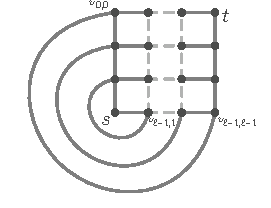
\includegraphics[scale=1,page=1]{networkAnalyzes/figures/ExtendedGridGraph.pdf}
    % 
    \caption[An extended grid graph.]{%
        % 
        An extended grid graph~$\glssymbol{graph}_{\mathrm{ex}}^\ell$ with
        a grid of dimension~$\ell\times\ell$ and~$\ell^2$ vertices.
        %
        \vspace*{-1.0cm}
    }%
    % 
    \label{ch:network-analysis:fig:extended-grid-graph}%
    % 
\end{wrapfigure}% 
% 
\noindent column~$0$ of the grid to a vertex~$\vertex_{\ell-1,i}$ on the bottom
border (see~\cref{ch:network-analysis:fig:extended-grid-graph}) such that either
the source~\source or the sink~\sink is located on the inner face
(in~\cref{ch:network-analysis:fig:extended-grid-graph} the source~\source is on
the inner face). We illustrated such a
graph~$\glssymbol{graph}_{\mathrm{ex}}^\ell$
in~\cref{ch:network-analysis:fig:extended-grid-graph}.
% 
\begin{lemma}[{{\parencite[p.145; Lemma~13]{Tru89}}}]
    % 
    Any plane graph~\glssymbol{graph} with~$(\source,\sink)\in\glssymbol{edges}$
    and with one of the two terminals (\ie, source~\source or sink~\sink) on the
    outer face, is a minor of some extended grid
    graph~$\glssymbol{graph}_{\mathrm{ex}}^\ell$ with~$\ell \geq 2$.
    % 
    \label{ch:network-analyzes:sec:mathematical-model:lem:plane-graph-grid-graphs}
    % 
\end{lemma}
% 
Note that it is always possible to use the inverse of all reduction rules
but~\cref{ch:network-analyzes:sec:mathematical-model:sim:star-polygon-transformation}.
In the following, we try to embed the graph~\glssymbol{graph} such that the
embedding has the form of an extended grid graph. We need the concept of a face
in the following
(\cref{ch:network-analyzes:sec:mathematical-model:subsec:planar-graphs}). For a
plane graph~\glssymbol{graph} a face~\cycle is a region that is bounded by the
edges and vertices of~\glssymbol{graph}. Two faces are incident if they share at
least one edge.
% 
\begin{lemma}
    % 
    Any plane \source-\sink-electrical-network~\glssymbol{network} with at least
    one terminal on the outer face can be embedded into a grid
    in~$\bigO(\fmagnitude{\glssymbol{vertices}})$ time.
    % 
    \label{ch:network-analyzes:sec:mathematical-model:lemma:embedding-into-a grid}
    % 
\end{lemma}
% 
\begin{figure}[t!]
    % 
    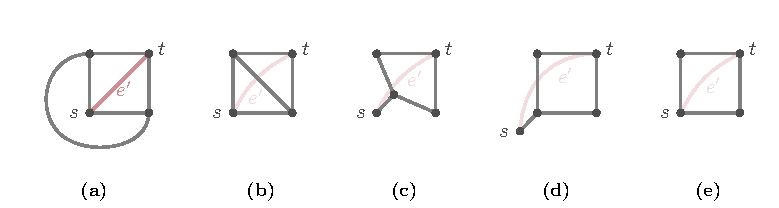
\includegraphics{networkAnalyzes/figures/Delta-Wye-Reducibility-Case-1.pdf}
    % 
    \caption[The delta-wye-reducibility of the smallest extended grid graph.]{A
    graph with four vertices, five edges, and one additional edge~$\edge' =
    (\source,\sink) \in \glssymbol{edges}$. The shown steps represent the
    reduction of the smallest possible extended grid
    graph~$\glssymbol{graph}_{\mathrm{ex}}^\ell$ with~$\ell = 2$. The steps are
    given in~\textcite{Tru89} for graphs in general. From (a) to (b) we just
    swap the outer edge to the inner face. From (b) to (c), we do a triangle to
    star transformation
    (see~\cref{ch:network-analyzes:sec:mathematical-model:sim:deltawye_transformation})
    of the lower left triangle. In the last step from (d) to (e), we do a series
    contraction
    (see~\cref{ch:network-analyzes:sec:mathematical-model:sim:series_contraction})
    and contract the edge in the bottom left with~$\edge'$. To contract the
    remaining graph to one edge~$\edge'=\{\source,\sink\}$, we do two series
    contractions and one parallel contraction.
    % 
    }
    %
    % Delta-Wye-Reducibility case 1 
    \label{ch:network-analyzes:sec:mathematical-model:fig:delta-wye-reducibility-case-1}
    % 
\end{figure}
% 
\begin{proof}
Note that the maximum degree of a grid graph~$
    % 
    \glssymbol{graph}_{\mathrm{grid}} 
    = 
    (
    \glssymbol{vertices}_{\mathrm{grid}},
    \glssymbol{edges}_{\mathrm{grid}}
    )
    % 
$ is at most~$4$. Thus, we split all vertices~$
    % 
    \vertex \in \glssymbol{vertices}(\glssymbol{graph})
    % 
$ with degree of at least~$
    % 
    \degree(\vertex)\geq 5
    % 
$. With~$\degree(\vertex)\leq 2 n_\vertex + 2$, we split them into~$
    % 
    n_\vertex 
    =
    \ceil{\nicefrac{\degree(\vertex)-2}{2}}
    =
    \ceil{\nicefrac{\degree(\vertex)}{2}}-1
    % 
$ vertices~$\vertex_i$ with $1\leq i \leq n_\vertex$ with~$
    % 
    \glssymbol{vertices}_{\vertex} 
    \coloneqq
    \left\{
        % \bigcup_{1\leq i \leq n_\vertex}
        \vertex_i
        \mid
        1\leq i \leq n_\vertex,
        \vertex\in\glssymbol{vertices} \colon
        \degree(\vertex) \geq 5
    \right\}
    % 
$ such that~$
    % 
    \glssymbol{vertices}_{\mathrm{grid}} 
    = 
    % \left\{
        \bigcup_{
            \{
                \vertex
                \in
                \glssymbol{vertices}
                \mid
                \degree(\vertex) \geq 5
            \}
        }
        \glssymbol{vertices}_{\vertex} 
    \cup
    \left(
        \glssymbol{vertices}(\glssymbol{graph})
        \setminus
        \{\vertex\}
    \right)
    % 
$ and~$
    % 
    \glssymbol{edges}_{\mathrm{grid}} 
    = 
    \glssymbol{edges}(\glssymbol{graph})
    \cup
    \big\{
        \{\vertex_i, \vertex_{i+1}\}
        \mid
        \vertex_i, \vertex_{i+1}\in\glssymbol{vertices}_{\vertex},
        \forall
        \vertex
        \in
        \glssymbol{vertices}_{\mathrm{grid}} 
        \setminus
        \glssymbol{vertices}(\glssymbol{graph})
    \big\}
    % 
$ with susceptance~$
    % 
    \glssymbol{susceptance}(\edge)
    =
    \infty
    % 
$ with~$
    % 
    \edge
    \in
    \glssymbol{edges}_{\mathrm{grid}}
    \setminus
    \glssymbol{edges}(\glssymbol{graph})
    % 
$. We set the susceptance to infinity such that~$
    % 
    \glssymbol{voltageangledifference}(\vertex_i,\vertex_{i+1})
    =
    \nicefrac{
        \glssymbol{flow}(\vertex_i,\vertex_{i+1})
    }{
        \glssymbol{susceptance}(\vertex_i,\vertex_{i+1})
    }
    =
    \nicefrac{
        \glssymbol{flow}(\vertex_i,\vertex_{i+1})
    }{
        \infty
    }
    \approx
    0
    % 
$ meaning that the voltage angles~$\glssymbol{voltageangle}(\vertex_i)$ are the
same for all~$\vertex_i\in\glssymbol{vertices}_{\vertex}$ with~$1\leq i\leq
n_{\vertex}$. Since the average degree of a finite plane graph is strictly less
than~$6$, we get~$2$ new vertices per vertex on average and thus, we
have~$\bigO(\fmagnitude{\glssymbol{vertices}})$ vertices.

Assume an arbitrary planar embedding of~$\glssymbol{graph}_{\mathrm{grid}}$.
Thus, we choose an inner face~$\cycle_{\source_1}$ that is incident to the
vertex~\source and choose a cut in the dual graph~$S\subseteq\glssymbol{edges}$
between~$\cycle_{\source_1}$ and the outer face~$\cycle_{o}$. Let~$
    % 
    \glssymbol{graph}_{\mathrm{grid}}' 
    =
    (
        \glssymbol{vertices}_{\mathrm{grid}}',
        \glssymbol{edges}_{\mathrm{grid}}'
    )
    % 
$ be a new graph with vertex set~$
    % 
    \glssymbol{vertices}' 
    =
    \glssymbol{vertices}
    \cup
    \{\source'\}
    % 
$ and edge set~$
    % 
    \glssymbol{edges}(\glssymbol{graph}') 
    =
    \glssymbol{edges}(\glssymbol{graph})
    \cup
    \big\{
        \{\source,\source'\}
    \big\}
    \setminus 
    S
    % 
$ with~$\glssymbol{susceptance} (\source,\source') = \infty$. This graph can be
embedded in~$
    % 
    \bigO(
        \fmagnitude{\glssymbol{vertices}}
    )
    % 
$ time into a grid of size at
most~$
    % 
    \fmagnitude{\glssymbol{vertices}}
    \times
    \fmagnitude{\glssymbol{vertices}}
    % 
$ using, \eg, the algorithm of~\textcite{Bie98}. Thus, we need~$
    % 
    \bigO(\fmagnitude{\glssymbol{vertices}}^2)
    % 
$ space.
This takes~$\bigO(\fmagnitude{\glssymbol{vertices}})$ time.
% 
\end{proof}
% 
% -Sch\"affter showed that is possible to draw any graph onto a~$2n\times 2n$ grid
% with at most 2 bends per edge "Drawing graphs on rectangular grids"
% - graphs with max degree 3 can be embedded in an 
% % $\ceil{\frac{n}{2}}\times\ceil{\frac{n}{2}}$ grid with~$\ceil{\frac{n}{2}}+2$ bends
% if the graph is planar it can be embedded in an $n\times n$ grid with $2n+4$
% bends if biconnected and $2.4n+2$ bends otherwise [23,25]
% - choose an arbitrary planar embedding of \glssymbol{graph}
% - choose an incident face of t as outer-face
% - choose a vertex s not = t on the outer-face
% - obtain a st-ordering
% 
We note that the outer edges that make the grid graph into an extended grid
graph
can be added by applying the following steps: 
% 
We add the remaining edges in~$S$. We place~$\source'$ on the bottom left
corner. Each time we add an edge~$
    % 
    \{\vertexa,\vertexb\}
    \in
    \glssymbol{undirectededges}
    % 
$ we check if~$\vertexa_{i_{\vertexa},0} = \vertexb_{\ell-1,i_{\vertexb}}$. If
neither is true then we add~$i_{\vertexb} - i_{\vertexa}$ new rows 
if~$i_{\vertexa}<i_{\vertexb}$ or new columns if~$i_{\vertexb}<i_{\vertexa}$.

Every plane electrical network can be embedded into a grid by using the
aforementioned algorithm. Thus, we make use of the following lemma.
% 
\begin{lemma}[{{\parencite[pp.142ff.; Theorem~2 \& Lemma~14]{Tru89}}}]
    % 
    Every (extended) grid graph with one source and one sink is 1-edge
    reducible.
    % 
    \label{ch:network-analyzes:sec:mathematical-model:lem:grid-graph-deltawye-reducible}
    % 
\end{lemma}
% 
So far we explained the different parts of the algorithm. Note that we assume a
plane~\source-\sink-graph~\glssymbol{graph} for the
algorithm. The algorithm (see~\cref{ch:network-analyzes:algo:s-t-power-flow-transformation-algorithm}) works as follows.
From~\cref{ch:network-analyzes:sec:mathematical-model:lemma:embedding-into-a
grid,ch:network-analyzes:sec:mathematical-model:lem:grid-graph-deltawye-reducible},
we know that any plane graph can be embedded into a grid
(see~\cref{ch:network-analyzes:algo:s-t-power-flow-transformation-algorithm}~\cref{ch:network-analyzes:algo:stpf:gridEmbedding})
and that every grid graph can be contracted to a single edge~$\edge'$
(see~\cref{ch:network-analyzes:algo:s-t-power-flow-transformation-algorithm}~\cref{ch:network-analyzes:algo:stpf:contractGridGraphToEdge}
and~\cref{ch:network-analyzes:sec:mathematical-model:fig:delta-wye-reducibility-case-1}).
In each~\deltawye-reduction, we compute the susceptances by the aforementioned
rules
(see~\cref{ch:network-analyzes:sec:mathematical-model:sim:deltawye_transformation,ch:network-analyzes:sec:mathematical-model:sim:wyedelta_transformation}).
% 
In the decontraction step
(see~\cref{ch:network-analyzes:algo:s-t-power-flow-transformation-algorithm}~\cref{ch:network-analyzes:algo:stpf:decontractGridGraphToEdge}),
we compute based on the given susceptances on the different contraction levels
the voltage angles~$\gls{voltageangle}(\vertexa)$
with~$\vertexa\in\gls{vertices}_i$ and the flow for each contraction level~$i$.
We start with~$\gls{network}_k$ consisting of a single edge~$\edge'$,
over~$\gls{network}_{k-1}$, and in the end we compute the voltage angles and the
flow for the original network~$\gls{network}_0$. For each level transition, we
apply the reverse of the applied transformation rules given
in~\cref{ch:network-analyzes:sec:mathematical-model:sim:series_contraction,ch:network-analyzes:sec:mathematical-model:sim:parallel_contraction,ch:network-analyzes:sec:mathematical-model:sim:loop_contraction,ch:network-analyzes:sec:mathematical-model:sim:degree_1_contraction,ch:network-analyzes:sec:mathematical-model:sim:deltawye_transformation,ch:network-analyzes:sec:mathematical-model:sim:wyedelta_transformation}.
% 
Note from~\cref{ch:network-analyzes:sec:mathematical-model:lem:rescalling-an-pf}
on 
Page~\pageref{ch:network-analyzes:sec:mathematical-model:lem:rescalling-an-pf}
that the capacities can be neglected, since we are always able to rescale a 
nontrivial electrical flow. This rescaling is not necessary
for~\gls{dc}~\gls{feas}, since a capacity violation would imply a non-existing
feasible electrical flow. However, assume that we apply an arbitrary flow
on~$\edge'$
(see~\cref{ch:network-analyzes:algo:s-t-power-flow-transformation-algorithm}~\cref{ch:network-analyzes:algo:stpf:flowAssignment})
resulting in an electrical flow that is not necessarily feasible, since the
capacity constraint might be violated. To fix the violation, we
use~\cref{ch:network-analyzes:sec:mathematical-model:lem:rescalling-to-mpf} on
Page~\pageref{ch:network-analyzes:sec:mathematical-model:lem:rescalling-to-mpf}
on the decontracted graph~\glssymbol{graph} with flow~\glssymbol{flow} to
rescale the flow to a feasible, \eg~\gls{mpf} 
(see~\cref{ch:network-analyzes:algo:s-t-power-flow-transformation-algorithm}~\cref{ch:network-analyzes:algo:stpf:rescaling}).
From~\textcite{Tru89}, we get the following running time.
% 
\begin{figure}[t!]
    % 
    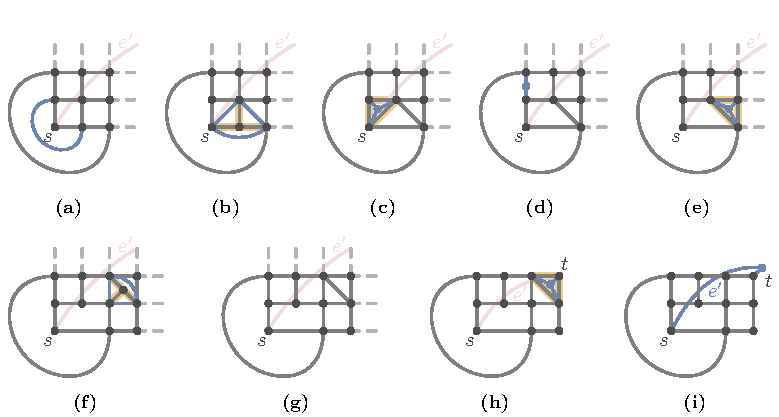
\includegraphics{networkAnalyzes/figures/Delta-Wye-Reducibility-Case-2.pdf}
    % 
    \caption[The delta-wye-reducibility of a general extended grid graph.]{A
    general extended grid graph~$\glssymbol{graph}_{\mathrm{ex}}^\ell$
    with~$\ell^2$ vertices. Blue edges and blue vertices represent the edges and
    vertices of the transformation and replace the orange marked edges. The
    steps are basically given by~\textcite{Tru89} for graphs in general. From
    (a) to (b) we use the steps already shown
    in~\cref{ch:network-analyzes:sec:mathematical-model:fig:delta-wye-reducibility-case-1}.
    % 
    }    % Delta-Wye-Reducibility case 2
    \label{ch:network-analyzes:sec:mathematical-model:fig:delta-wye-reducibility-case-2}
    % 
\end{figure}

\begin{lemma}
    % 
    The algorithm runs in~$\bigO(\fmagnitude{\glssymbol{vertices}}^3)$ time. 
    % and
    % needs~$\bigO(\fmagnitude{\glssymbol{vertices}}^2)$ space.
    % 
    \label{ch:network-analyzes:sec:mathematical-model:obs:arbitrary-capacities}
    % 
\end{lemma}
% 
% Algo decontraction notes:\\
% - note that the voltage angles in a parallel decontraction stay the same as the
% edge itself\\
% - In a series contraction however these angles do not change either, but the
% inner vertices get a voltage angle between the outer ones\\
% - the voltage angles at the triangle vertices stay the same in
% \deltawye-contraction and thus \wyedelta-decontraction do not change voltage
% angles at all\\
% - in the \wyedelta-contraction and thus, \deltawye-decontraction we have to
% calculate the center new, but in  single-source and single-sink graphs the
% voltage angle is equivalent to one of the triangle ones, since the flow is
% zero\\
The contraction step of the
algorithm~\cref{ch:network-analyzes:algo:s-t-power-flow-transformation-algorithm}~\cref{ch:network-analyzes:algo:stpf:contractGridGraphToEdge}
is illustrated
in~\cref{ch:network-analyzes:sec:mathematical-model:fig:delta-wye-reducibility-case-1,ch:network-analyzes:sec:mathematical-model:fig:delta-wye-reducibility-case-2}
for an extended grid graph.
% 
\begin{lemma}
    A planar~\source-\sink-graph~\glssymbol{graph} can always be contracted to one
    edge by a series of reduction rules (see~\parencite{Tru89}).
    % 
    \label{ch:network-analyzes:sec:mathematical-model:con:planar-graph-single-edge}
\end{lemma}
% 
For the reverse operation, we remark that the voltage angles in a parallel and
series contraction do not change. For the series contraction, we have to compute
the voltage angles for the inner vertices
using~\cref{ch:network-analyzes:sec:mathematical-model:eq:kvl-ohm-function-writing}.
For the~\deltawye- and~\wyedelta-transformation, the voltage angles at the three
outer vertices do not change. For the center of the star, we have to compute the
voltage angle
using~\cref{ch:network-analyzes:sec:mathematical-model:eq:kvl-ohm-function-writing}.
The reconstruction steps can be done during the recursive return. If the
capacities are violated, we rescale the flow~\glssymbol{flow}
using~\cref{ch:network-analyzes:sec:mathematical-model:lem:rescalling-an-pf}.
From the previous discussion follows the next theorem.
% 
\begin{theorem}
    The algorithm computes a feasible electrical flow for a
    planar~\source-\sink-graph~\glssymbol{graph}.
    % 
    \label{ch:network-analyzes:sec:mathematical-model:thm:algo-pf-1}
\end{theorem}
% 
% \franzi{Cholesky Factorization}
% \franzi{Conjugate Gradient and Precondioned Conjugate Gradient -> Improve
% Preconditioners by using the structure from this and the section before }
% \franzi{
%     * We can probably improve the bounds for linear solvers, since we know what preconditioners they would like to have
%     * They use as preconditioners minimum fundamental weighted bases. 
%     * From the structure we observed in the beginning, we know that the fundamental is not necessary. 
%     * Thus, we do not need to solve an NP-hard problem, but one that is easy to solve and where polynomial time algorithm exist such as Horton and the improvements from Mehlhorn.
% }
% 
%%%%%%%%%%%%%%%%%%%%%%%%%%%%%%%%%%%%%%%%%%%%%%%%%%%%%%%%%%%%%%%%%%%%%%%%%%%%%%%
\section{Representations and Formulations of Electrical Flows}
\label{ch:network-analyzes:sec:representations}
%%%%%%%%%%%%%%%%%%%%%%%%%%%%%%%%%%%%%%%%%%%%%%%%%%%%%%%%%%%%%%%%%%%%%%%%%%%%%%%
% 
\textcite[p.13]{Cai12} mention that power grids are planar
(see~\cref{ch:network-analyzes:sec:mathematical-model:subsec:planar-graphs}) and
undirected. Recall from~\cref{ch:foundations:sec:graph-theory} that we can
transform any undirected graph to a directed graph, which we do for notational
conveniences. The planarity of graph~\glssymbol{graph} is a crucial property of
the network~\glssymbol{network} for this section. In addition, we assume that
the graph~\glssymbol{graph} is biconnected.
% 
%%%%%%%%%%%%%%%%%%%%%%%%%%%%%%%%%%%%%%%%%%%%%%%%%%%%%%%%%%%%%%%%%%%%%%%%%%%%%%%% 
\subsection{The Duality Concept for Graphs}
\label{ch:network-analyzes:sec:duality-concept}
%%%%%%%%%%%%%%%%%%%%%%%%%%%%%%%%%%%%%%%%%%%%%%%%%%%%%%%%%%%%%%%%%%%%%%%%%%%%%%%%
% 
Using the duality of the incidence matrix~\glssymbol{incidenceMatrix} and
circuit matrix~\glssymbol{cycleMatrix} that was shown
in~\cref{ch:network-analyzes:sec:mathematical-model:subsec:matroids-independence-systems},
we translate the algebraic duality of the two matrices into a graph theoretical
duality
(\cref{ch:network-analyzes:sec:mathematical-model:subsec:planar-graphs}). Recall
that a base of a
matroid~(see~\cref{ch:network-analyzes:sec:mathematical-model:def:base}) is a
maximum independent set. The complement of a base in the primal
graph~\glssymbol{graph} is the base in the dual graph~\glssymbol{dualgraph}
(see~\cref{ch:network-analyzes:sec:mathematical-model:cor:incidence-circuit-matrix-duals}).
% 
\begin{theorem}[{{\parencite[p.522; Theorem 23]{Whi35}}}]
    % 
    Let~$\glssymbol{embedding}$ be a planar embedding of a
    graph~\glssymbol{graph}. The graphs~\glssymbol{graph}
    and~\glssymbol{dualgraph} are duals if and only if there is a bijection~$
        % 
        \oneToOneMap
        \colon
        \glssymbol{edges}(\glssymbol{graph}) 
        \to
        \glssymbol{edges}(\glssymbol{dualgraph})
        % 
    $ between their edges such that bases in one correspond to base complements
    in the other.
    % 
    \label{ch:network-analyzes:sec:mathematical-model:thm:Matroids-one-to-one-corrspondence}
    % 
\end{theorem}
% 
The construction
in~\cref{ch:network-analyzes:sec:mathematical-model:subsec:planar-graphs}
implies a bijection of edges in the primal graph~\glssymbol{graph} to edges in
its dual graph~\glssymbol{dualgraph}.
% 
It is called a combinatorial dual in terms of the Whitney duality (bijection of
edges; and a set of edges forming a cut corresponds to a cycle
in the combinatorial dual). Note that the dual of a dual
graph~\glssymbol{dualgraph} is isomorphic to the primal graph~\gls{graph} as
long as~\glssymbol{graph} is connected.

From~\crefrange{ch:network-analyzes:sec:mathematical-model:eq:KCL-intermediate-vertex}{ch:network-analyzes:sec:mathematical-model:eq:KCL-consumer-vertex}, we know
that a feasible~\gls{kcl} flow on the primal graph~\gls{graph} is equivalent to
a graph theoretical flow in the primal graph~\gls{graph}.
% 
It follows
from~\cref{ch:network-analyzes:sec:mathematical-model:cor:incidence-circuit-matrix-duals}
that a feasible~\gls{kvl} flow corresponds to a graph theoretical flow in the
dual graph. Thus, we get the following lemma.
% 
\begin{lemma}
    % 
    A feasible~\gls{kvl} flow~$\glssymbol{flow}_{\glssymbol{graph}}$ in the
    primal graph~\glssymbol{graph} is equivalent to a feasible~\gls{kcl}
    flow~$\glssymbol{flow}_{\glssymbol{dualgraph}}$ in the corresponding dual
    graph~\glssymbol{dualgraph}.
    % 
    \label{ch:network-analyzes:sec:mathematical-model:lem:KVL-flow-in-dual}
    % 
\end{lemma}
% 
Note that we can apply any flow~\glssymbol{flow} on a self-loop~$
    % 
    \edge 
    =
    (\vertexa,\vertexa)
    % 
$, since it is redundant. Thus, we get the following observation.
% 
\begin{observation}
    % 
    Let the primal graph~\glssymbol{graph} be a tree. Thus, there is only one
    face that is equivalent to the outer-face~$\cycle_t$. The dual graph
    consists of self-loops only. Let~\glssymbol{flow} be any feasible flow
    on~\glssymbol{graph}. Then, flow~\glssymbol{flow} is also a feasible
    electrical flow.
    % 
    \label{ch:network-analyzes:sec:mathematical-model:eq:bnorm}
    % 
\end{observation}
%
Recall from~\cref{ch:network-analyzes:sec:reduction-transformation-rules} that
every self-loop can be removed
(see~\cref{ch:network-analyzes:sec:mathematical-model:sim:loop_contraction}).
The aforementioned observation is a geometrical explanation for planar graphs of
the results of~\textcite[p.9; Lemma 4]{Leh15a} and~\textcite{Lei15b} that on
trees any graph-theoretical flow is also electrical feasible.

We note that a series contraction
(see~\cref{ch:network-analyzes:sec:mathematical-model:sim:series_contraction})
in~\glssymbol{graph} is an equivalent transformation to the parallel contraction
(see~\cref{ch:network-analyzes:sec:mathematical-model:sim:parallel_contraction})
in the dual graph~\glssymbol{dualgraph}. We highlight that by the following
structural observation.
% 
\begin{observation}
    The series contraction in the primal graph~\glssymbol{graph} is equivalent to the parallel
    contraction in its dual~\glssymbol{dualgraph} and vice versa.
    \label{ch:network-analyzes:sec:mathematical-model:obs:parallel-series-duality}
\end{observation}
% 
\begin{observation}
    The~\deltawye-transformation in the primal graph~\glssymbol{graph} is equivalent to
    the~\wyedelta-transformation in the dual graph~\glssymbol{dualgraph} and
    vice versa.
    \label{ch:network-analyzes:sec:mathematical-model:obs:deltawye-wyedelta-duality}
\end{observation}
% 
In the following section, we will make use of the duality by reformulating the
problem.
% 
%%%%%%%%%%%%%%%%%%%%%%%%%%%%%%%%%%%%%%%%%%%%%%%%%%%%%%%%%%%%%%%%%%%%%%%%%%%%%%%%
% 
\begin{figure}[t!]
    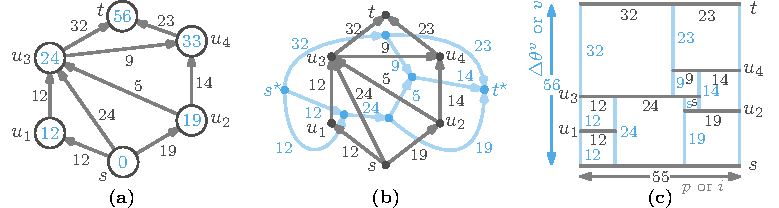
\includegraphics[page=1]{networkAnalyzes/figures/AnalogiesFlowDualSquares.pdf}
    % 
    \caption[Different representation for the power flow feasibility problem.]
    {We use the example graph of~\textcite[p.18]{Fel13}. The susceptances
    are~$\textcolor{SUSCEPTANCE}{\glssymbol{susceptance} \equiv 1}$, the
    feasible electrical flow~$\textcolor{PRIMALGRAPH}{\glssymbol{flow}(\edge)}$
    is written on each edge~$\edge\in\glssymbol{edges}$, and we neglect the
    capacities meaning~$\textcolor{CAPACITY}{\glssymbol{capacity}\equiv\infty}$.
    (a) The example graph's feasible electrical flow is in this case the minimum
    integer feasible electrical flow~\textcolor{PRIMALGRAPH}{\glssymbol{flow}}
    and the corresponding voltage
    angles~\textcolor{THETA}{\glssymbol{voltageangle}}. (b) The
    flow~\textcolor{PRIMALGRAPH}{\glssymbol{flow}} and the voltage angle
    differences~\textcolor{THETA}{\glssymbol{voltageangledifference}} can be
    separated into two graphs, which are the primal graph~\textcolor{KITblack50}
    {\glssymbol{graph}} and its dual
    graph~\textcolor{DUALGRAPH}{\glssymbol{dualgraph}}, respectively. (c) Since
    the susceptances are~$\textcolor{SUSCEPTANCE}{\glssymbol{susceptance} \equiv
    1}$ a similar representation is a squaring of
    a~$\textcolor{PRIMALGRAPH}{55}\times\textcolor{DUALGRAPH}{56}$ rectangle,
    where the \textcolor{PRIMALGRAPH}{width} and the
    \textcolor{DUALGRAPH}{height} of each square is represented by the flow in
    the \textcolor{PRIMALGRAPH}{primal} and \textcolor{DUALGRAPH}{dual graph},
    respectively. Each vertex in the \textcolor{PRIMALGRAPH}{primal} and
    \textcolor{DUALGRAPH}{dual graph} represents a
    \textcolor{PRIMALGRAPH}{horizontal} or \textcolor{DUALGRAPH}{vertical
    segment}, respectively. For clarity we labeled the vertices for the primal
    graph only, since otherwise this figure seems overloaded. An edge represents
    a side of a square. }
    % 
    \label{ch:network-analyzes:fig:AnalogiesFlowDualSquares}
    % 
\end{figure}
% 
% 
%%%%%%%%%%%%%%%%%%%%%%%%%%%%%%%%%%%%%%%%%%%%%%%%%%%%%%%%%%%%%%%%%%%%%%%%%%%%%%%% 
\subsection{Simultaneous Flow Representation}
\label{ch:network-analyzes:simultaneous-flow-representation}
%%%%%%%%%%%%%%%%%%%%%%%%%%%%%%%%%%%%%%%%%%%%%%%%%%%%%%%%%%%%%%%%%%%%%%%%%%%%%%%%
% 
We use the aforementioned duality and structure of the problem to
reformulate~\gls{dc}~\gls{feas} in terms of the~\emph{\acrlong{sfp}}
(\gls{sfp}). For~\gls{sfp} the graphs are not necessarily duals, but share some
edges.
% 
\begingroup
    %%%%%%%%%%%%%%%%%%%%%%%%%%%%%%%%%%% Problem %%%%%%%%%%%%%%%%%%%%%%%%%%%%%%%%%%%%
\begin{problem}[framed]{
% 
\acrlong{sfp}~\footnote{After showing our results to Guido Br\"uckner, he
mentioned the~\gls{sfp} generalization to us. We would like to thank him for
that generalization of the biconnected
planar~\source-\sink-\gls{dc}~\gls{feas}-problem.}~$\gls{sfp}(
\glssymbol{network})$
% 
}%
% 
% 
  Instance: & Two graphs~$\glssymbol{graph}_1$ and~$\glssymbol{graph}_2$,
  subsets $
    % 
    \glssymbol{edges}_1
    \subseteq
    \glssymbol{edges}(\glssymbol{graph}_1)
    % 
  $ and~$
    % 
    \glssymbol{edges}_2
    \subseteq
    \glssymbol{edges}(\glssymbol{graph}_2)
    % 
  $, and a bijection~$
    % 
    % \oneToOneMap
    \foneToOneMap{\gls{sfp}}
    \colon 
    \glssymbol{edges}_1 
    \to
    \glssymbol{edges}_2$.
  % 
  \\
  % 
  Question: & Are there nonzero~\gls{kcl}-feasible flows~$
    % 
    \glssymbol{flow}_{\glssymbol{graph}_1}
    % 
  $ and~$
    % 
    \glssymbol{flow}_{\glssymbol{graph}_2}
    % 
  $ in~$\glssymbol{graph}_1$ and~$\glssymbol{graph}_2$  
  % 
  % with~$\glssymbol{flowvalue}(\glssymbol{graph}_1)\not=0$ and~$
  % \glssymbol{flowvalue}(\glssymbol{graph}_2)\not=0$ 
  %  
  such that for every edge~$\edge\in\glssymbol{edges}_1$ we have~$
    % 
    \glssymbol{flow}_{\glssymbol{graph}_1}(\edge) 
    =
    \glssymbol{flow}_{\glssymbol{graph}_2}(\foneToOneMap{\gls{sfp}}(\edge))
    % 
  $?
\end{problem}%
%%%%%%%%%%%%%%%%%%%%%%%%%%%%%%%%%%%%%%%%%%%%%%%%%%%%%%%%%%%%%%%%%%%%%%%%%%%%%%%%
    \label{ch:networkAnalysis:problems:SimultaneousFlowProblem-Decision_Problem}
\endgroup
%
The reformulation of~\gls{dc}~\gls{feas} separates the
constraints---meaning~\gls{kcl} and~\gls{kvl}---by the usage of two graphs,
which we define in the following. Recall that our graph is planar and
biconnected, and that we denote by~$\oneToOneMap\colon \glssymbol{edges}
(\glssymbol{graph}(\glssymbol{embedding}))\to \glssymbol{edges}(
\glssymbol{dualgraph})$ the bijection of the edges
with~$\edge_i\mapsto\oneToOneMap(\edge_i) = \edge_i^\star$. An
edge~$(\vertexa,\vertexc) = \edge_i \in\glssymbol{graph}$ corresponds to an edge
$(\cycle_1,\cycle_2)=\edge_i^\star\in\glssymbol{dualgraph}$ and vice versa if
and only if $\edge_i$ is incident to both faces~$\cycle_1$ and~$\cycle_2$, and
$\edge_i^\star$ is incident to the faces~\vertexa and~\vertexc. Since there is
no unique embedding of a biconnected planar graph the mapping is not unique.
This means that the bijection is always related to some planar embedding of
graph~\glssymbol{graph}.

Without loss of generality, we assume that flow~$\glssymbol{flow}$ is a
function~$\glssymbol{flow}\colon\glssymbol{edges}\to\integers$. Recall that we
can always rescale~\glssymbol{flow} to a feasible electrical flow that is
non-integral (meaning~$\glssymbol{flow}\colon\glssymbol{edges}\to\reals$) by
using the scaling
from~\cref{ch:network-analyzes:sec:mathematical-model:lem:rescalling-an-pf}.

From~\cref{ch:network-analyzes:sec:mathematical-model:thm:matrix-and-its-circuit-matrix-are-duals},
we know that a graph's base of the incidence matrix and the corresponding base
of the circuit matrix are duals. Given a graph and its dual, we know
from~\cref{ch:network-analyzes:sec:mathematical-model:cor:incidence-circuit-matrix-duals}
that the incidence matrix of either graphs is equivalent to the circuit matrix
of the other, whereby equivalent means here that an edge-cut at a vertex in one
graph represents a simple cycle in the other graph and vice versa. The latter
means that for a spanning tree~\tree in graph~\glssymbol{graph} the set~$
    % 
    \glssymbol{edges}' 
    = 
    \glssymbol{edges}(\glssymbol{graph})
    \setminus
    \glssymbol{edges}(\tree)
    % 
$ of chords in one graph corresponds to a set~$
    \glssymbol{edges}'' 
    =
    \{
        \oneToOneMap(\edge)
        \mid
        \edge
        \in
        \glssymbol{edges}'
    \}
    % 
$ of edges in the dual graph, where~$\glssymbol{edges}''$ constitutes a tree.
Now,
\cref{ch:network-analyzes:sec:mathematical-model:thm:Matroids-one-to-one-corrspondence}
and~\cref{ch:network-analyzes:sec:mathematical-model:lem:KVL-flow-in-dual} can
be used to transform~\gls{dc}~\gls{feas} in terms of simultaneous flows. An edge
cut~\glssymbol{cuts} at vertex~$
% 
\vertexa
\in
\glssymbol{vertices}(\glssymbol{dualgraph})
% 
$ with~$
% 
\glssymbol{cuts}(\vertexa)
=
\{
    \edge
    \in
    \glssymbol{undirectededges}(\glssymbol{dualgraph})
    \mid
    \vertexa
    \in
    \edge
\}
% 
$ is a cycle~\glssymbol{cycle} in the biconnected planar
graph~$\glssymbol{graph}$. A conservation of flow at~\vertexa means that the
incoming flow is equivalent to the outgoing flow. For the corresponding
cycle~\glssymbol{cycle} this means that flows along the cycle sum up to zero.
Note that a flow direction in~\glssymbol{graph} corresponds to a flow direction
in~\glssymbol{dualgraph} and vice versa.

The following problem is equivalent to~\gls{dc}~\gls{feas} on~\source-\sink
plane graphs.
%
\begingroup
    %%%%%%%%%%%%%%%%%%%%%%%%%%%%%%%%%%% Problem %%%%%%%%%%%%%%%%%%%%%%%%%%%%%%%%%%%%
\begin{problem}[framed]{\source-\sink Planar~\gls{dc}~\gls{feas}(\glssymbol{network})
 % \&~\source-\sink Planar~\gls{mpfp}(\glssymbol{network}) 
 % 
 % $\source-\sink P~\gls{dc}~\gls{feas}(\glssymbol{network})$
 % $\source-\sink P~\gls{mpfp}(\glssymbol{network})$
 % 
 }%
  Instance: & A plane~\source-\sink-graph~\glssymbol{graph}, its
  dual graph~\glssymbol{dualgraph}, and the corresponding
  bijection~$\oneToOneMap\colon \glssymbol{edges}(\glssymbol{graph}) \to
  \glssymbol{edges}(\glssymbol{dualgraph})$.
  \\
  % 
  Question: & Are there simultaneous flows on~\glssymbol{graph}
  and~\glssymbol{dualgraph} such that~$
  % 
  \glssymbol{flow}_{\glssymbol{graph}}(\edge) 
  = 
  \glssymbol{flow}_{\glssymbol{dualgraph}}
  \big(
    \oneToOneMap(\edge)
  \big)
  \cdot
  \glssymbol{susceptance}(\edge)
  % 
  $ for all~$\edge\in\glssymbol{edges}(\glssymbol{graph})$?
\end{problem}%
    \label{ch:networkAnalysis:problems:DC_FEAS_simultaneous_flow-Decision_Problem}
\endgroup
% 
In the objective of the reformulated \source-\sink planar~\gls{dc}~\gls{feas}
and~\gls{dc}~\gls{mpfp}, we can easily see that this is a restatement
of~\cref{ch:network-analyzes:sec:mathematical-model:eq:kvl-ohm-function-writing}
by replacing the phase angle difference~$\glssymbol{voltageangledifference}
(\vertexa,\vertexc)\coloneqq\glssymbol{voltageangle}(\vertexc)-
\glssymbol{voltageangle}(\vertexa)$ with the flow in the dual
graph~$\glssymbol{flow}_{\glssymbol{dualgraph}}(\oneToOneMap(\edge))$ with~$\edge =
(\vertexa,\vertexc)\in\glssymbol{edges}$. An example for the reformulation is
given in~\cref{ch:network-analyzes:fig:AnalogiesFlowDualSquares}\screen{b}.
In~\cref{ch:network-analyzes:fig:AnalogiesFlowDualSquares}\screen{a}
and~\screen{b} an electrical flow with its unique voltage angle assignment and
its translation to simultaneous flows is shown, respectively. Using simultaneous
flows~\cref{ch:network-analyzes:sec:mathematical-model:eq:kvl-ohm-function-writing}
becomes~\cref{ch:network-analyzes:eq:KVL-reformulation}.
% 
\begin{equation}
    \glssymbol{flow}_{\glssymbol{graph}}(\edge) 
    =
    \glssymbol{flow}_{\glssymbol{dualgraph}} 
    \big(\oneToOneMap(\edge)\big)
    \cdot
    \glssymbol{susceptance}(\edge)
    % 
    \qquad\qquad
    \forall \edge \in \glssymbol{edges}
    % 
    \label{ch:network-analyzes:eq:KVL-reformulation}
\end{equation}
% 
Roughly speaking, the susceptance~\glssymbol{susceptance} represents a gear
ratio between the primal graph's flow~$\glssymbol{flow}_{\glssymbol{graph}}$ and
the dual graph's flow~$\glssymbol{flow}_{\glssymbol{dualgraph}}$. 
% 
\begin{theorem}
    A flow~\glssymbol{flow} in~\glssymbol{graph} is an electrical flow if and
    only if the primal flow~$\glssymbol{flow}_{
    \glssymbol{graph}}\equiv\glssymbol{flow}$ and the
    flow~$\glssymbol{flow}_{\glssymbol{dualgraph}}$ in the dual
    graph~\glssymbol{dualgraph} comply the flow conservation (\gls{kcl}) and if
    for every edge~$\edge\in\glssymbol{edges}$ the flow
    complies~$\glssymbol{flow}_{\glssymbol{graph}}(\edge) =
    \glssymbol{flow}_{\glssymbol{dualgraph}}\big(\oneToOneMap
    (\edge)\big)\cdot\glssymbol{susceptance}(\edge)$.
    % 
    \label{ch:network-analyzes:thm:electrical-flow-based-definition}
\end{theorem}
% 
\begin{proof}
    The left-hand side
    of~\cref{ch:network-analyzes:thm:electrical-flow-based-definition:1}
    and~\cref{ch:network-analyzes:thm:electrical-flow-based-definition:2} comes
    from~\cref{ch:network-analyzes:sec:mathematical-model:eq:kcl-matrix-writing}
    and~\cref{ch:network-analyzes:sec:mathematical-model:eq:kvl-matrix-writing},
    respectively. Recall that we can
    reformulate~\cref{ch:network-analyzes:sec:mathematical-model:eq:kvl-matrix-writing}
    with~$
        % 
        \glssymbol{cycleMatrix}(\glssymbol{graph})
        \cdot
        \vv{\glssymbol{voltageangledifference}} 
        =
        \vv{0}
        % 
    $ in terms of flows
    using~\cref{ch:network-analyzes:sec:mathematical-model:eq:voltage-angle-diff-replacement-to-flows:allg}
    with~$
        % 
        \glssymbol{cycleMatrix}'(\glssymbol{graph})
        \cdot
        \vv{\glssymbol{flow}} 
        =
        \vv{0}
        % 
    $.
    From~\cref{ch:network-analyzes:sec:mathematical-model:cor:incidence-circuit-matrix-duals},
    we know that the incidence matrix~\glssymbol{incidenceMatrix} and the
    circuit matrix~\glssymbol{cycleMatrix} are duals meaning~$
        % 
        \glssymbol{incidenceMatrix}(\glssymbol{graph}) 
        = 
        \glssymbol{cycleMatrix}'(\glssymbol{dualgraph})
        % 
    $ and~$
        % 
        \glssymbol{cycleMatrix}'(\glssymbol{graph}) 
        = 
        \glssymbol{incidenceMatrix}(\glssymbol{dualgraph})
        % 
    $. Using the duality, we get
    for~\cref{ch:network-analyzes:sec:mathematical-model:eq:kcl-matrix-writing}
    and~\cref{ch:network-analyzes:sec:mathematical-model:eq:kvl-matrix-writing}
    the following.
    % 
    % 
    % From~\cref{ch:network-analyzes:sec:mathematical-model:thm:Matroids-one-to-one-corrspondence}
    % and~\cref{ch:network-analyzes:sec:mathematical-model:thm:basis-contain-no-cylces}
    % follows the equivalence given for the incidence
    % matrix~$\glssymbol{incidenceMatrix}(\glssymbol{graph})$ and the circuit
    % matrix~$\glssymbol{cycleMatrix}(\glssymbol{graph})$ of the primal
    % graph~\glssymbol{graph} 
    % in~\cref{ch:network-analyzes:thm:electrical-flow-based-definition:1}
    % and~\cref{ch:network-analyzes:thm:electrical-flow-based-definition:2},
    % respectively.
    % 
    \begin{subequations}
    \begin{align}
        % 
        \glssymbol{incidenceMatrix}(\glssymbol{graph})\cdot 
        \hspace{1mm}
        \vv{\glssymbol{flow}_{\glssymbol{graph}}}
        &=
        % \frighthandsidevector{\glssymbol{incidenceMatrix}}
        \vv{0}
        % 
        &\Leftrightarrow&\hspace{0.5cm}
        % 
        \glssymbol{cycleMatrix}(\glssymbol{dualgraph})\cdot
        \vv{\glssymbol{voltageangledifference}_{\glssymbol{dualgraph}}}
        &=
        \vv{0}
        % 
        \label{ch:network-analyzes:thm:electrical-flow-based-definition:1}
        % 
        \\
        % 
        \glssymbol{cycleMatrix}(\glssymbol{graph})\cdot
        \vv{\glssymbol{voltageangledifference}_{\glssymbol{graph}}}
        &=
        \vv{0}
        % 
        &\Leftrightarrow&\hspace{0.5cm}
        % 
        \glssymbol{incidenceMatrix}(\glssymbol{dualgraph})\cdot 
        \hspace{1mm}
        \vv{\glssymbol{flow}_{\glssymbol{dualgraph}}}
        &=
        % \frighthandsidevector{\glssymbol{incidenceMatrix}}
        \vv{0}
        % 
        \label{ch:network-analyzes:thm:electrical-flow-based-definition:2}
        % 
    \end{align}
    \label{ch:network-analyzes:thm:electrical-flow-based-definition}
    \end{subequations}
    % 
    % We define~$
    % % 
    %     \glssymbol{voltageangledifference}
    %     \equiv
    %     \glssymbol{flow}_{\glssymbol{dualgraph}}
    % % 
    % $. From the aforementioned equivalence and
    % using~\cref{ch:network-analyzes:sec:mathematical-model:eq:voltage-angle-diff-replacement-to-flows:allg},
    % we get the following relationship.
    % 
    % \begin{align}
    %     \glssymbol{incidenceMatrix}(\glssymbol{graph})
    %     \cdot
    %     \vv{\glssymbol{flow}}_{\glssymbol{graph}}
    %     &=
    %     \glssymbol{cycleMatrix}(\glssymbol{dualgraph})
    %     \cdot
    %     \vv{\glssymbol{voltageangledifference}}_{\glssymbol{dualgraph}}
    %     % 
    %     \label{ch:network-analyzes:sec:mathematical-model:eq:thm:1.48:a}
    %     \\
    %     &=
    %     \glssymbol{cycleMatrix}(\glssymbol{dualgraph})
    %     \cdot
    %     (
    %         \vv{x}
    %         \circ
    %         \vv{\glssymbol{flow}}_{\glssymbol{graph}}
    %     )
    %     % 
    %     \label{ch:network-analyzes:sec:mathematical-model:eq:thm:1.48:b}
    %     \\
    %     \glssymbol{incidenceMatrix}(\glssymbol{graph})
    %     &=
    %     \glssymbol{cycleMatrix}(\glssymbol{dualgraph})
    %     \circ    
    %     (
    %         \mathbb{1}^{ 
    %             \fmagnitude{\glssymbol{edges}} 
    %             \times 
    %             1 
    %         }
    %         \cdot
    %         \transpose{ \vv{\glssymbol{reactance}} }
    %     )
    %     % 
    %     \label{ch:network-analyzes:sec:mathematical-model:eq:thm:1.48:c}
    %     \\
    %     \glssymbol{incidenceMatrix}(\glssymbol{graph})
    %     &=
    %     \glssymbol{cycleMatrix}'(\glssymbol{dualgraph})
    %     % 
    %     \label{ch:network-analyzes:sec:mathematical-model:eq:thm:1.48:d}
    % \end{align}
% 
% 
    % From the aforementioned equation, we get the following
    % 
    % get the relationships of the flows
    % and voltage angle differences 
    % in~\cref{ch:network-analyzes:thm:electrical-flow-based-definition:4-5}. 
    % 
    % \cref{ch:network-analyzes:sec:mathematical-model:eq:voltage-angle-diff-replacement-to-flows:allg}
    %
    % \begin{subequations}
    % \begin{align}
    %     \glssymbol{flow}_{\glssymbol{graph}}(\edge) 
    %     &=
    %     \glssymbol{voltageangledifference}_{\glssymbol{dualgraph}}(\oneToOneMap(\edge)) 
    %     % 
    %     &\forall \edge \in \glssymbol{edges}(\glssymbol{graph})
    %     % 
    %     \label{ch:network-analyzes:thm:electrical-flow-based-definition:3}
    %     % 
    %     \\
    %     \glssymbol{flow}_{\glssymbol{dualgraph}}(\edge) 
    %     &=
    %     \glssymbol{voltageangledifference}_{\glssymbol{graph}}(\oneToOneMap^{-1}
    %     (\edge))
    %     % 
    %     &\forall \edge \in \glssymbol{edges}(\glssymbol{dualgraph})
    %     % 
    %     \label{ch:network-analyzes:thm:electrical-flow-based-definition:4}
    %     % 
    % \end{align}
    % \label{ch:network-analyzes:thm:electrical-flow-based-definition:4-5}
    % \end{subequations}
    % 
    % The aforementioned relationship is similar to the findings of~\textcite
    % [p.404, Section 3]{For56} introducing the duality between maximum flows and
    % shortest paths in which a minimum cut in~\glssymbol{graph} corresponds to a
    % shortest path in the dual graph~\glssymbol{dualgraph}. However, in our case
    % this relationship means that all paths are shortest paths. We discuss this
    % in more detail in~\cref{ch:network-analyzes:sec:balancing-property}.
    % 
    From~\cref{ch:network-analyzes:sec:mathematical-model:eq:kvl-ohm-function-writing}
    and~\cref{ch:network-analyzes:thm:electrical-flow-based-definition:2} we
    get~\cref{ch:network-analyzes:thm:electrical-flow-based-definition:5-6}.
    % 
    \begin{subequations}
    \begin{align}
        \glssymbol{flow}_{\glssymbol{graph}}(\edge) 
        &= 
        \glssymbol{susceptance}(\edge)\cdot
        \glssymbol{voltageangledifference}_{\glssymbol{graph}}(\edge)
        % 
        \label{ch:network-analyzes:thm:electrical-flow-based-definition:5}
        \\
        \glssymbol{flow}_{\glssymbol{graph}}(\edge) 
        &= 
        \glssymbol{susceptance}(\edge)\cdot
        \glssymbol{flow}_{\glssymbol{dualgraph}}(\oneToOneMap(\edge)) 
        % 
        \label{ch:network-analyzes:thm:electrical-flow-based-definition:6}
    \end{align}
    \label{ch:network-analyzes:thm:electrical-flow-based-definition:5-6}
    \end{subequations}
    % 
    % \cref{ch:network-analyzes:thm:electrical-flow-based-definition:6} concludes
    % our proof. 
    The illustration of the relationship is given
    in~\cref{ch:network-analyzes:fig:AnalogiesSusceptanceScaling}.
\end{proof}
% 
Another equivalent representation is given
in~\cref{ch:network-analyzes:fig:AnalogiesFlowDualSquares}\screen{c}, which we
describe in the following.
% 
%%%%%%%%%%%%%%%%%%%%%%%%%%%%%%%%%%%%%%%%%%%%%%%%%%%%%%%%%%%%%%%%%%%%%%%%%%%%%%%% 
\subsection{Rectangular Representation}
\label{ch:network-analyzes:rectangular-representation}
%%%%%%%%%%%%%%%%%%%%%%%%%%%%%%%%%%%%%%%%%%%%%%%%%%%%%%%%%%%%%%%%%%%%%%%%%%%%%%%%
% 
Another representation of simultaneous flows was given by~\textcite[p.18]{Fel13}
and is shown
in~\cref{ch:network-analyzes:fig:AnalogiesFlowDualSquares}\screen{c}. We note
that this is basically an adopted idea of~\textcite{Ros86} that use a similar
construction for rectilinear planar layouts but do not use it for a squaring of
an outer rectangle.
% 
This representation is in general denoted by \emph{rectangular
dissection}~\rectangulardissection. Within this representation a vertex is
either a horizontal or vertical line segment dependent on whether the vertex is
in the primal graph~\glssymbol{graph} or dual graph~\glssymbol{dualgraph}.
In~\cref{ch:network-analyzes:fig:AnalogiesFlowDualSquares}\screen{c}, a
horizontal segment corresponds to a vertex in the primal graph~\glssymbol{graph}
and a vertical segment corresponds to a vertex in the dual
graph~\glssymbol{dualgraph}. We illustrate the latter
in~\cref{ch:network-analyzes:fig:AnalogiesFlowDualSquares}\screen{c} for the
primal graph by labeling the segments with the corresponding
vertices~$\source,\vertexa_1,\vertexa_2,\vertexa_3,\vertexa_4,\sink\in
\glssymbol{vertices}$. An edge represents a side of a square. Dependent on the
graph a flow on that edge affects either the horizontal or vertical side ratio
(\ie, the width or height of a rectangle).

\citeauthor{Fel13} shows that a special case of simultaneous flow can be
represented by squaring of an outer rectangle. The case
in~\cref{ch:network-analyzes:fig:AnalogiesFlowDualSquares}\screen{c} shows such
a special case, where all inner partitions of an outer rectangle are squares.
The reason for that is that the susceptance~\glssymbol{susceptance} is~$
\glssymbol{susceptance}\equiv 1$ and thus,
\cref{ch:network-analyzes:eq:KVL-reformulation} becomes~$
% 
\glssymbol{flow}_{\glssymbol{graph}}(\edge) 
=
\glssymbol{flow}_{\glssymbol{dualgraph}}
\big(\oneToOneMap(\edge)\big)
% 
$ for all~$\edge\in\glssymbol{edges}$. 

However, a more general definition that is closer to power grids would be to
allow arbitrary susceptances~$\glssymbol{susceptance}(\undirectededge)$
with~$\undirectededge\in\glssymbol{undirectededges}$. Than the representation is
not a \emph{squaring} of an outer rectangle. Meaning that the inner partitions
are not necessary squares, but can be rectangles with differing aspect ratio
dependent on the susceptance~\glssymbol{susceptance}. An example is given
in~\cref{ch:network-analyzes:fig:AnalogiesSusceptanceScaling}.

Note that
from~\cref{ch:network-analyzes:sec:mathematical-model:lem:KVL-flow-in-dual} we
know that a feasible flow in the primal graph~\glssymbol{graph} models the
actual (power) flow that is equivalent to a current flow~\glssymbol{current}
(see~\cref{ch:foundations:sec:power-flow-analyses:analogies-to-the-dc-model} on
Page~\pageref{ch:foundations:sec:power-flow-analyses:analogies-to-the-dc-model})
and that a feasible flow in the dual graph~\glssymbol{dualgraph} models the
voltage angle differences~$\glssymbol{voltageangledifference}$ that is
equivalent to the voltage drops~$\glssymbol{voltage}$
(see~\cref{ch:foundations:sec:power-flow-analyses:analogies-to-the-dc-model} on
Page~\pageref{ch:foundations:sec:power-flow-analyses:analogies-to-the-dc-model}).
Recall that a flow~$
\glssymbol{flow}_{\glssymbol{graph}}$ in the primal
graph~\glssymbol{graph} represents one side of the rectangle
(in~\cref{ch:network-analyzes:fig:AnalogiesSusceptanceScaling}\screen{c} this
would be the width) and the~$\glssymbol{flow}_{\glssymbol{dualgraph}}$ in the
dual graph~\glssymbol{dualgraph} represents the other side of the rectangle
(in~\cref{ch:network-analyzes:fig:AnalogiesSusceptanceScaling}\screen{c} this
would be the height). Thus, the surface of a rectangle represents the
power~$\glssymbol{realpower}$, which explains the quadratic relationship
(see~\cref{ch:network-analyzes:obs:quadratic-relationship}).
%
\begin{lemma}
    The primal graph~\glssymbol{graph} and the dual graph~\glssymbol{dualgraph}
    model the quadratic relationship between voltage~\glssymbol{voltage}
    and current~\glssymbol{current} meaning~$\glssymbol{realpower} =
    \glssymbol{voltage}\cdot\glssymbol{current}$
    (see~\cref{ch:foundations:sec:power-flow-analyses:eq:complex-power-vi}).
    % 
    \label{ch:network-analyzes:obs:quadratic-relationship}
    % 
\end{lemma}
% 
\textcite[p.8]{Fel13} restricted~\rectangulardissection to the case, where there
is no point where four rectangles meet each other. However,
in~\cref{ch:network-analyzes:fig:AnalogiesSusceptanceScaling}\screen{c} we can
see that this is possible and does not cause any problem. Such a representation
can be also seen as a segment contact representation. We refer for the latter
representation to~\textcite{Fel13}.
% 
% To draw squarings of a rectangle without demands this might lead to
% exponential size drawings showing that the given graph represents a bad
% squaring. 
% Note that constructing a squaring is in general~\NP-hard~\parencite{Oer14} as it
% falls in the category of switching (see~\cref{ch:switching}) and~\gls{tnep}.

For a given graph the drawing of a squaring of rectangles is unique, which
follows from~\cref{ch:network-analyzes:sec:mathematical-model:lem:unique-flow}.
% 
In~\cref{ch:network-analyzes:sec:bipolar-orientation}, we will see that a
bipolar orientation exists if the graph is biconnected. The embedding of
biconnected planar graph is not unique, since we can switch for example the
order of parallel paths. However,
from~\cref{ch:network-analyzes:sec:mathematical-model:lem:unique-flow} we know
that the flows are unique.
% 
\begin{lemma}[Unique Partition of a Rectangular Representation]
    The rectangles of a rectangular representation have unique minimum integral
    sizes. The embedding of these rectangles can vary.
    % 
    \label{ch:network-analyzes:lem:unique-partition-rectangular-representation}
\end{lemma}
% 
This concludes a very important property of simultaneous flows and a rectangular
representation. 
% In addition, we can restrict the size of such a drawing by the
% result given in~\cref{ch:network-analyzes:sec:mathematical-model:lem:integral-e-flow-poly-size}.
% 
% \begin{lemma}
%     The size of the rectangular representation is polynomial in the input size. 
%     % 
%     \label{ch:network-analyzes:sec:representation:rectangular:lem:size}
% \end{lemma}
% 
These representations separates the quadratic relationship and help to
understand important properties of electrical flows, which we will see in the
next section. In the following, we will discuss the balancing property that will
be used as a criteria for termination and basically describes the conflict
resolution in each graph.
% 
\begin{figure}
    % 
    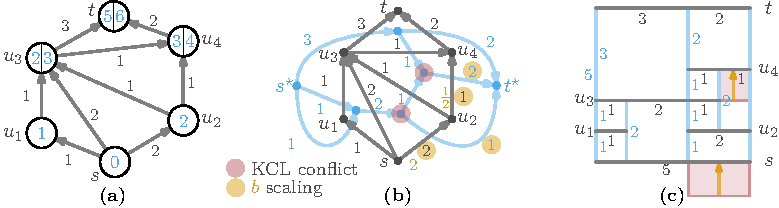
\includegraphics[page=1]{networkAnalyzes/figures/AnalogiesSusceptanceScaling.pdf}
    % 
    \caption[The geometric interpretation of a susceptance scaling.]{We use the
    example graph of~\textcite[p.18]{Fel13} that is also used
    in~\cref{ch:network-analyzes:fig:AnalogiesFlowDualSquares}. The
    \textcolor{SUSCEPTANCE}{susceptances}
    are~$\textcolor{SUSCEPTANCE}{\glssymbol{susceptance}\equiv 1}$ and we
    neglect the \textcolor{CAPACITY}{capacities} meaning~$\textcolor{CAPACITY}{
    \glssymbol{capacity}\equiv\infty}$. We write the flows~\glssymbol{flow} on
    the edges or on the rectangle's side. (a) We apply some feasible
    flow~\textcolor{PRIMALGRAPH}{\glssymbol{flow}} (\ie, complying the~\gls{kcl}
    and capacity constraints only)
    on~\textcolor{PRIMALGRAPH}{graph~\glssymbol{graph}}. The feasible
    flow~\textcolor{PRIMALGRAPH}{\glssymbol{flow}} is not a feasible electrical
    flow, since the voltage angles (distance
    labels))~\textcolor{THETA}{\glssymbol{voltageangle}} at the
    vertices~\tikzVertex are not unique. The latter can be seen in the double
    assignments at~$\vertexa_3,\vertexa_4,\sink\in\glssymbol{vertices}$. Thus,
    the~\gls{kvl} is violated. (b) It is always possible to transform a feasible
    flow~\textcolor{PRIMALGRAPH}{\glssymbol{flow}} into a feasible electrical
    flow~$\textcolor{PRIMALGRAPH}{\glssymbol{flow}'}$ by scaling the
    susceptances~$\textcolor{SUSCEPTANCE}{\glssymbol{susceptance}}$ at certain
    edges such that the
    ratio~$\nicefrac{\textcolor{PRIMALGRAPH}{\glssymbol{flow}}}
    {\textcolor{DUALGRAPH}{\glssymbol{voltageangledifference}}} \equiv
    \nicefrac{\textcolor{PRIMALGRAPH}{\glssymbol{flow}_{\glssymbol{graph}}}}{
    \textcolor{DUALGRAPH}{\glssymbol{flow}_{\glssymbol{dualgraph}}}}
    \equiv \textcolor{SUSCEPTANCE}{\glssymbol{susceptance}}$ changes the flow~$
    \textcolor{DUALGRAPH}{\glssymbol{flow}_{\glssymbol{dualgraph}}}$ in such a
    way that it becomes feasible (\ie, complying~\gls{kcl} and thus, \gls{kvl})
    as long as the \textcolor{SUSCEPTANCE}{susceptance~\glssymbol{susceptance}}
    is not restricted
    meaning~$\textcolor{SUSCEPTANCE}{\glssymbol{susceptance}\in[0,\infty]}$. (c)
    In the geometric setting a \textcolor{SUSCEPTANCE}{susceptance} scaling
    represents an aspect ratio scaling (indicated by the
    \textcolor{SUSCEPTANCE}{arrows $\uparrow$}). The bottom right box would
    exceed the outer rectangle by one unit without the susceptance scaling
    of~$\textcolor{SUSCEPTANCE}{2}$. Without the susceptance scaling of~$
    \textcolor{SUSCEPTANCE}{\nicefrac{1} {2}}$ there would be a gap of one unit
    in the right center.}
    % 
    \label{ch:network-analyzes:fig:AnalogiesSusceptanceScaling}
\end{figure}
% 
%%%%%%%%%%%%%%%%%%%%%%%%%%%%%%%%%%%%%%%%%%%%%%%%%%%%%%%%%%%%%%%%%%%%%%%%%%%%%%%
\section{The Balancing Property}
\label{ch:network-analyzes:sec:balancing-property}
%%%%%%%%%%%%%%%%%%%%%%%%%%%%%%%%%%%%%%%%%%%%%%%%%%%%%%%%%%%%%%%%%%%%%%%%%%%%%%%
% 
Electrical flows have a property of balancing meaning the flows do not congest
certain edges but spread the load over multiple paths from~\source to~\sink.
Note that this is the main difference to graph-theoretical flows that
try---while maximized---to congest all edges as much as possible. The balancing
property of electrical flows is equivalent to flows that minimize the total
losses (\cref{ch:network-analyzes:eq:minimize-losses-quadratic-eq}).
% 
\begin{equation}
    % 
    \min~\sum_{\edge\in\glssymbol{undirectededges}}
    \nicefrac{\glssymbol{flow}(\edge)^2}{\glssymbol{susceptance}(\edge)},
    % 
    \label{ch:network-analyzes:eq:minimize-losses-quadratic-eq}
\end{equation}
% 
which is a quadratic function~\parencite[p.275; Section~2.2, Energy
Equation]{Chr11}. In this section, we describe this property in terms of
simultaneous flows using algorithmic properties that exploit the aforementioned
structure (see~\cref{ch:network-analyzes:obs:quadratic-relationship})

\textcite[p.404; Section~3]{For56} introduced the duality between maximum flows
and shortest paths in which a minimum cut in~\glssymbol{graph} corresponds to a
shortest path in the dual graph~\glssymbol{dualgraph}. To use shortest paths, we
first introduce a distance metric for power grids. The distance between two
vertices is usually the length of an edge or time to pass that edge. The
distance in an electrical network, is given by the potential
difference~$
    % 
    \glssymbol{voltageangle}(\vertexc) 
    -
    \glssymbol{voltageangle}(\vertexa)
    % 
$ that is the voltage angle difference~$
    % 
    \glssymbol{voltageangledifference}(\vertexa,\vertexc)
    % 
$.
 
For a given flow~\glssymbol{flow} the voltage angle difference on
any~\vertexa-\vertexc-path~$\fpath{}{\vertexa}{\vertexc}$ is given
in~\cref{ch:network-analyzes:sec:mathematical-model:eq:actual-voltage-angle-difference}
and is derived
from~\cref{ch:network-analyzes:sec:mathematical-model:eq:kvl-ohm-function-writing}.
We now give a generalization of the voltage angle difference~$
\glssymbol{voltageangledifference}$ that is original defined on edges to the
voltage angle difference on paths that is a distance
function~$\glssymbol{voltageangledifference}\colon\glssymbol{pathset}\to\mathbb{F}$,
where~$
\mathbb{F}$ is a field (\eg, \reals) and~$\glssymbol{pathset}$ is a set of
paths. Note that the equations that are build
from~\cref{ch:network-analyzes:sec:mathematical-model:eq:actual-voltage-angle-difference}
constitute a matrix and the generalization is a simple sum of the rows that
result
in~\cref{ch:network-analyzes:sec:mathematical-model:eq:kvl-ohm-function-writing}.
%
\begin{equation}
    \glssymbol{voltageangledifference}(\fpath{}{\vertexa}{\vertexc})
    \coloneqq
    \sum_{(i,j)\in\fpath{}{\vertexa}{\vertexc}}\frac{\glssymbol{flow}(i,j)}
    {\glssymbol{susceptance}(i,j)},
    % 
    \label{ch:network-analyzes:sec:mathematical-model:eq:actual-voltage-angle-difference}
\end{equation}
% 
for a path~$\fpath{}{\vertexa}{\vertexc}\in\glssymbol{pathset}$
with~$\vertexa,\vertexc\in\glssymbol{vertices}$. 
% 
For electrical flows the metric is~$\nicefrac{\glssymbol{flow}(\edge)}{
\glssymbol{susceptance}(\edge)}$ deduced from~\cref{ch:network-analyzes:sec:mathematical-model:eq:actual-voltage-angle-difference}.
% 
The~\acrlong{sppp} (\gls{sppp}) computes a path with minimum length~$
\fpath{\gls{spp}}{\source}{\sink}\coloneqq$
$\min_{\fpath{}{\source}{\sink}\in\glssymbol{pathset}} $
$\sum_{\edge\in\fpath{}{\source}{\sink}}$
$\nicefrac{\glssymbol{flow}(\edge)}{\glssymbol{susceptance}(\edge)}
$. Contrary, the~\acrlong{lppp} (\gls{lppp}) computes a
path that has the longest distance between two vertex pairs~$
\fpath{\gls{lpp}}{\source}{\sink}\coloneqq $
$\max_{\fpath{}{\source}{\sink}\in\glssymbol{pathset}}$
$\sum_{\edge\in\fpath{}{\source}{\sink}}$
$\nicefrac{\glssymbol{flow}(\edge)}{\glssymbol{susceptance}(\edge)}$.  

From the previous section (see
especially~\cref{ch:network-analyzes:sec:mathematical-model:eq:kvl-matrix-writing,ch:network-analyzes:sec:mathematical-model:eq:kvl-ohm-function-writing})
we know that the voltage angle assignments are unique and thus, we get the
following observation that is illustrated
in~\cref{ch:network-analyzes:fig:LongestVsShortestPathAnalogies}.

The distance between to vertices~$\vertexa,\vertexc\in\glssymbol{vertices}$
with~$(\vertexa,\vertexc)\in\glssymbol{edges}$ is given by the voltage angle
difference~$
% 
\glssymbol{voltageangledifference}(\vertexa,\vertexc) 
\coloneqq
\glssymbol{voltageangle}(\vertexc) - \glssymbol{voltageangle}(\vertexa)
% 
$ with voltage angles~\glssymbol{voltageangle} that can be interpreted as 
distance labels. The voltage angle difference (\ie, the electrical distance)
for a path~$\glssymbol{path}(\source,\sink)$ is given by~$
\glssymbol{voltageangledifference}(\glssymbol{path}(\source,\sink))
\!=\!
\sum_{(\vertexa,\vertexc)\in\glssymbol{path} (\source,\sink)}\! 
\glssymbol{voltageangledifference}(\vertexa,\vertexc) 
\!=\!
\sum_{(\vertexa,\vertexc)\in\glssymbol{path}(\source,\sink)}\! 
\nicefrac{\glssymbol{flow}(\vertexa,\vertexc)}{
\glssymbol{susceptance}(\vertexa,\vertexc)}
$.
% 
\begin{lemma}[Balancing Flow Property]
    Given a primal graph~\glssymbol{graph} and its dual
    graph~\glssymbol{dualgraph}, for which the shortest path~$
    % 
        \fpath{
            \gls{spp}
        }{\source}{\sink}
        \in
        \glssymbol{pathset}(\glssymbol{graph})
    % 
    $ in~\glssymbol{graph} (respectively longest path~$
        % 
        \fpath{
            \gls{lpp}
        }{\source}{\sink}
        \in
        \glssymbol{pathset}(\glssymbol{graph})
        % 
    $) can differ to the shortest path~$
    % 
        \fpath{
            \gls{spp}
        }{\source}{\sink}
        \in
        \glssymbol{pathset}(\glssymbol{dualgraph})
    % 
    $ 
    in~\glssymbol{dualgraph} (respectively longest path~$
        % 
        \fpath{
            \gls{lpp}
        }{\source}{\sink}
        \in
        \glssymbol{pathset}(\glssymbol{dualgraph})
        % 
    $). A flow~\glssymbol{flow} is an electrical flow if and only if the longest
    and shortest path have the same length~$
    % 
        \glssymbol{voltageangledifference}(\fpath{\gls{spp}}{\source}{\sink})
        = 
        \glssymbol{voltageangledifference}(\fpath{\gls{lpp}}{\source}{\sink})
    % 
    $ in~$\glssymbol{graph}$
    with~$\source,\sink\in\glssymbol{vertices}(\glssymbol{graph})$ and~$
    % 
        \glssymbol{voltageangledifference}(
            \fpath{\gls{spp}}{\source^\star}{\sink^\star}
        )
        = 
        \glssymbol{voltageangledifference}(
            \fpath{\gls{lpp}}{\source^\star}{\sink^\star}
        )
    % 
    $ in~$\glssymbol{dualgraph}$
    with~$\source^\star,\sink^\star\in\glssymbol{vertices}(\glssymbol{dualgraph})$
    (\wrt~the distance
    metric~$\nicefrac{\glssymbol{flow}}{\glssymbol{susceptance}}$).
    % 
    \label{ch:network-analyzes:lem:balancing-flow-property}
\end{lemma}
% 
\begin{proof}
    $\Rightarrow\colon$ 
    % 
    First we show the one direction, where~\glssymbol{flow} is a feasible
    electrical flow, which implies that the length of all paths is equivalent~$
        \glssymbol{voltageangledifference}(\fpath{\gls{spp}}{\source}{\sink})
        =
        \glssymbol{voltageangledifference}(\fpath{\gls{lpp}}{\source}{\sink})
    $.

    Let~\glssymbol{flow} be a feasible electrical flow. 
    If~$
        % 
        \glssymbol{voltageangledifference}(\fpath{\gls{spp}}{\source}{\sink}) 
        \neq
        \glssymbol{voltageangledifference}(\fpath{\gls{lpp}}{\source}{\sink}) 
        % 
    $ in~\glssymbol{graph} with~$
    \source,
    \sink
    \in
    \glssymbol{vertices}(\glssymbol{graph})
    % 
    $ then there is no unique voltage angle
    assignment~$\glssymbol{voltageangle}(\vertexa)$ for all~$\vertexa\in
    \glssymbol{vertices}(\glssymbol{graph})$. This implies that~\glssymbol{flow}
    does not comply with the~\gls{kvl}
    (see~\cref{ch:network-analyzes:sec:mathematical-model:eq:kvl-ohm-function-writing}).
    If~$
        % 
        \glssymbol{voltageangledifference}(\fpath{\gls{spp}}{\source^\star}
        {\sink^\star})
        \neq
        \glssymbol{voltageangledifference}(\fpath{\gls{lpp}}{\source^\star}{\sink^\star})
        % 
    $ in~\glssymbol{dualgraph} with~$
    \source^\star,
    \sink^\star
    \in
    \glssymbol{vertices}(\glssymbol{dualgraph})
    % 
    $ then there is no unique voltage angle assignment in~\glssymbol{dualgraph} 
    (see~\cref{ch:network-analyzes:thm:electrical-flow-based-definition}), 
    % 
    which means that~\glssymbol{flow} does not comply with the~\gls{kcl}
    (see~\crefrange{ch:network-analyzes:sec:mathematical-model:eq:kcl-matrix-writing:1}{ch:network-analyzes:sec:mathematical-model:eq:kcl-matrix-writing:3}).
    Any one of the two cases would be a contradiction to~\glssymbol{flow} being
    a feasible electrical flow
    (see~\cref{ch:network-analyzes:sec:mathematical-model:def:kvl-kcl-feasible-flow}).

    $\Leftarrow\colon$
    With the other direction, we show that if~$
        % 
        \glssymbol{voltageangledifference}(\fpath{\gls{spp}}{\source}{\sink})
        =
        \glssymbol{voltageangledifference}(\fpath{\gls{lpp}}{\source}{\sink})
        % 
    $ then this implies that~\glssymbol{flow} is a feasible electrical flow.
    % 
    Given two paths from~\source to~\sink denoted by~$
        % 
        \fpath{1}{\source}{\sink},
        \fpath{2}{\source}{\sink}
        \in
        \glssymbol{pathset}
        % 
    $ that merge at vertex~$x$, meaning~$
        % 
        \fpath{1}{x}{\sink} 
        = 
        \fpath{2}{x}{\sink} 
        \eqqcolon 
        \glssymbol{path}
        % 
    $. In addition, we have given the distance metric~$
        % 
        \nicefrac{
            \glssymbol{flow}(\vertexa,\vertexc)
        }{
            \glssymbol{susceptance}(\vertexa,\vertexc)
        }
        % 
    $ then from~$
    % 
        \glssymbol{voltageangledifference}\big(\fpath{1}{\source}{\sink}\big)
        =
        \glssymbol{voltageangledifference}\big(\fpath{2}{\source}{\sink}\big)
    % 
    $ using the distance metric follows 
    % 
    \begin{align*}
        % 
        \sum_{(\vertexa,\vertexc)\in\fpath{1}{\source}{\sink}}
        \frac{
            \glssymbol{flow}(\vertexa,\vertexc)
        }{
            \glssymbol{susceptance}(\vertexa,\vertexc)
        }
        &=
        \sum_{(\vertexa,\vertexc)\in\fpath{2}{\source}{\sink}}
        \frac{
            \glssymbol{flow}(\vertexa,\vertexc)
        }{
            \glssymbol{susceptance}(\vertexa,\vertexc)
        }.
    \end{align*}
    % 
    We define the voltage angles on the source~\source and sink~\sink to
    be~$\glssymbol{voltageangle} (\source)\coloneqq 0$, and~$
    % 
        \glssymbol{voltageangle}(\sink)
        \coloneqq 
        \glssymbol{voltageangledifference}
        \big(
            \fpath{1}{\source}{\sink}
        \big)
        =
        \glssymbol{voltageangledifference}
        \big(
            \fpath{2}{\source}{\sink}
        \big)
    % 
    $. 

    \begin{align*}
        \glssymbol{voltageangle}(\source) 
        + 
        \sum_{ (\vertexa,\vertexc) \in \fpath{1}{\source}{x} }
        \frac{
            \glssymbol{flow}(\vertexa,\vertexc)
        }{
            \glssymbol{susceptance}(\vertexa,\vertexc)
        }
        +
        \glssymbol{path}
        =
        \glssymbol{voltageangle}(\sink)
        \\
        \glssymbol{voltageangle}(\source) 
        + 
        \sum_{ (\vertexa,\vertexc) \in \fpath{2}{\source}{x} }
        \frac{
            \glssymbol{flow}(\vertexa,\vertexc)
        }{
            \glssymbol{susceptance}(\vertexa,\vertexc)
        }
        +
        \glssymbol{path}
        =
        \glssymbol{voltageangle}(\sink)
    \end{align*}

    Since~$\glssymbol{path} = \fpath{1}{x}{\sink} = \fpath{2}{x}{\sink}$,
    $\glssymbol{voltageangle} (\source) = 0$, and the voltage angle~$
    % 
        \glssymbol{voltageangle}(\sink) 
        = 
        \glssymbol{voltageangledifference}
        \big(
            \fpath{1}{\source}{\sink}
        \big)
        = 
        \glssymbol{voltageangledifference}
        \big(
            \fpath{2}{\source}{\sink}
        \big)
    % 
    $. It follows that 
    \begin{align*}
        % 
        \sum_{(\vertexa,\vertexc)\in\fpath{1}{\source}{x}}
        \frac{
            \glssymbol{flow}(\vertexa,\vertexc)
        }{
            \glssymbol{susceptance}(\vertexa,\vertexc)
        }
        &=
        \sum_{(\vertexa,\vertexc)\in\fpath{2}{\source}{x}}
        \frac{
            \glssymbol{flow}(\vertexa,\vertexc)
        }{
            \glssymbol{susceptance}(\vertexa,\vertexc)
        }
        &=
        \glssymbol{voltageangle}(\sink) 
        -
        \glssymbol{voltageangle}(\source)
        -
        \glssymbol{path} 
        .
    \end{align*}
    % 
    Thus, the distances from the source~\source to the vertex~$x$ are the same
    meaning~$
    % 
        \glssymbol{voltageangledifference}\big(\fpath{1}{\source}{x}\big)
        $
        $
        =
        \glssymbol{voltageangledifference}\big(\fpath{2}{\source}{x}\big)
        \eqqcolon 
        \glssymbol{voltageangle}(x)
    % 
    $.
    % 
    We can recursively proceed, which gives us the following equality. 
    % 
    \begin{align*}
        % 
        \sum_{(\vertexa,\vertexc)\in\fpath{1}{\source}{x}}
        \glssymbol{voltageangledifference}(\vertexa,\vertexc)
        &=
        \sum_{(\vertexa,\vertexc)\in\fpath{2}{\source}{x}}
        \glssymbol{voltageangledifference}(\vertexa,\vertexc)
        % 
    \end{align*}
    % 
    This relationship is known
    from~\cref{ch:network-analyzes:sec:mathematical-model:eq:kvl-ohm-function-writing} 
    and restated by~$
    % 
        \glssymbol{voltageangledifference}(\vertexa,\vertexc)
        \coloneqq
        \big(
            \glssymbol{voltageangle}(\vertexc) 
            - 
            \glssymbol{voltageangle}(\vertexa)
        \big) 
        = \frac{
            \glssymbol{flow}(\vertexa,\vertexc)
        }{
            \glssymbol{susceptance}(\vertexa,\vertexc)
        }
    % 
    $.
    % 
    The phase angles on each side cancel each other out, but the source~\source
    and the sink~\sink.
    % 
    \begin{align*}
        \begin{aligned}
            \big(
                \glssymbol{voltageangle}(\vertexa_1) 
                - \glssymbol{voltageangle}(\source)
            \big)
            &+
            \big(
                \glssymbol{voltageangle}(\vertexa_2) 
                - 
                \glssymbol{voltageangle}(\vertexa_1)
            \big)
            &+&
            \big(
                \glssymbol{voltageangle}(\vertexa_3) 
                - 
                \glssymbol{voltageangle}(\vertexa_2)
            \big)
            +
            \dots
            \\
            % +
            \dots
            &+
            \big(
                \glssymbol{voltageangle}(\vertexa_n) 
                - 
                \glssymbol{voltageangle}(\vertexa_{n-1})
            \big)
            &+&
            \big(
                \glssymbol{voltageangle}(\vertexa_{\sink}) 
                - 
                \glssymbol{voltageangle}(\vertexa_n)
            \big)
            =
            \big(
                \glssymbol{voltageangle}({\sink}) 
                - 
                \glssymbol{voltageangle}({\source})
            \big)
        \end{aligned}
    \end{align*}
    % 
    Since the source~\source and the sink~\sink are for both
    paths~$\fpath{1}{\source}{\sink},\fpath{2}{\source}
    {\sink}\in\glssymbol{pathset}$ the same and both paths have the same
    distance~$
    % 
        \glssymbol{voltageangledifference}\big(\fpath{1}{\source}{\sink}\big)
        =
        \glssymbol{voltageangledifference}\big(\fpath{2}{\source}{\sink}\big)
    % 
    $ the voltage angle assignments are unique. We get
    $
    % \glssymbol{flow}(\source,\sink)
    % =
    % \glssymbol{susceptance}(\source,\sink)
    \big(
        \glssymbol{voltageangle}(\sink) 
        - 
        \glssymbol{voltageangle}(\source)
    \big) 
    =
    \sum_{(\vertexa,\vertexc)\in\fpath{1}{\source}{\sink}}
    \frac{
        \glssymbol{flow}(\vertexa,\vertexc)
    }{
        \glssymbol{susceptance}(\vertexa,\vertexc)
    }
    =
    \sum_{(\vertexa,\vertexc)\in\fpath{2}{\source}{\sink}}
    \frac{
        \glssymbol{flow}(\vertexa,\vertexc)
    }{
        \glssymbol{susceptance}(\vertexa,\vertexc)
    }
    = \frac{
        \glssymbol{flow}(\source,\sink)
    }{
        \glssymbol{susceptance}(\source,\sink)
    }.
    $

    % % 
    % From~\cref{ch:network-analyzes:sec:mathematical-model:eq:kvl-ohm-function-writing}
    % we know that~$
    % \glssymbol{voltageangledifference}(\vertexa,\vertexc)
    % \coloneqq
    % \big(
    %     \glssymbol{voltageangle}(\vertexc) 
    %     - 
    %     \glssymbol{voltageangle}(\vertexa)
    % \big) 
    % = \frac{
    %     \glssymbol{flow}(\vertexa,\vertexc)
    % }{
    %     \glssymbol{susceptance}(\vertexa,\vertexc)
    % }$. 
\end{proof}

\begin{figure}[t!]
    % 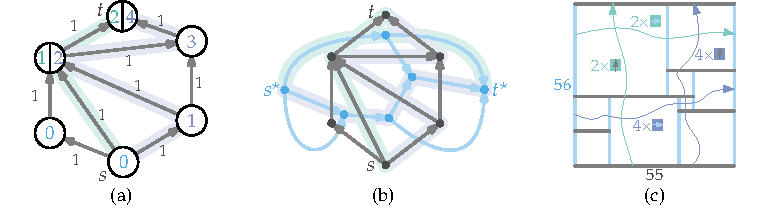
\includegraphics[page=1]{networkAnalyzes/figures/LongestVsShortestPathAnalogies.pdf}
    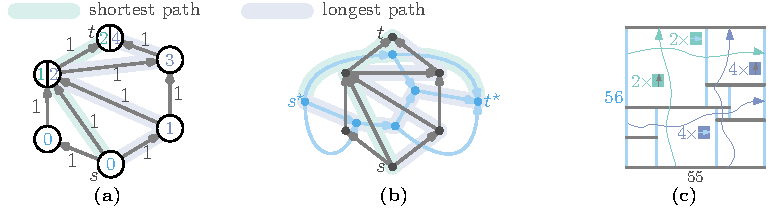
\includegraphics[page=1]{networkAnalyzes/figures/Property-of-Balancing.pdf}
    % 
    \caption[The property of balancing.]{We use the example graph
    of~\textcite[p.18]{Fel13}. The~\textcolor{SUSCEPTANCE}{susceptances
    are~$\glssymbol{susceptance}\equiv 1$} and we neglect the capacities
    meaning~\textcolor{CAPACITY}{$\glssymbol{capacity}\equiv\infty$}. (a)
    Assuming unit distances the \textcolor{KITgreen70}{shortest
    path~$\fpath{\gls{spp}}{\source}{\sink}$} and \textcolor{KITblue70}{longest
    path~$\fpath{\gls{lpp}}{\source}{\sink}$} in the original graph with the
    corresponding distance labels at the vertices have length
    \textcolor{KITgreen70}{2} and \textcolor{KITblue70}{4}, respectively. (b)
    The \textcolor{KITgreen70}{shortest} and \textcolor{KITblue70}{longest} path
    in the~\textcolor{PRIMALGRAPH}{primal graph~\glssymbol{graph}}
    and~\textcolor{DUALGRAPH}{dual graph~\glssymbol{dualgraph}} have the same
    length. However, adding an edge from~\source to~\sink describes that this is
    not always the case. (c) The \textcolor{KITgreen70}{shortest path~$
    \fpath{\gls{spp}}{\source}{\sink}$} and
    \textcolor{KITblue70}{longest path~$\fpath{\gls{lp}}{\source}{\sink}$}
    describe the \textcolor{KITgreen70}{minimum} and \textcolor{KITblue70}
    {maximum} number of rectangles (here squares) that are stacked in either
    directions.}
    % 
    \label{ch:network-analyzes:fig:LongestVsShortestPathAnalogies}
\end{figure}
% 
The intuition that electricity follows the path of the least resistance and
tries to balance itself leads us to a~\emph{balanced flow}, where all paths have
the same length from any vertex to any other vertex. First, we introduce
shortest paths for power grids that represent one part of the intuition namely
the path with the least resistance. Note that vertex label differences always
sum up to zero and thus, these labels, too. Recall that this is exactly the same
behavior as
in~\cref{ch:network-analyzes:sec:mathematical-model:eq:kvl-ohm-function-writing}
for the voltage angles.
% 
A vertex~\vertex that
violates~\crefrange{ch:network-analyzes:sec:mathematical-model:eq:kcl-matrix-writing:1}{ch:network-analyzes:sec:mathematical-model:eq:kcl-matrix-writing:3}
has an excess~$\glssymbol{netflow}(\vertex)\not= 0$. The excess represents the
amount of flow that has to be reduced or increased in~\vertex's incoming or
outgoing flow, respectively. From the duality of the~\acrlong{mfp}
and~\acrlong{sppp}~\parencite[p.404; Section~3]{For56} and the aforementioned
discussion on the duality of the~\gls{kcl} and~\gls{kvl} constraints, we get the
following observation.
%
\begin{observation}
A feasible~\gls{kvl} flow can be computed by a shortest path in the primal
graph~\glssymbol{graph}.
% 
\label{ch:network-analyzes:sec:mathematical-model:lem:KVL-voltage-angles}
\end{observation}
% 
Note that a feasible~\gls{kvl} flow is not restricted to shortest paths as long
as the voltage angle assignment is unique. Contrary a feasible~\gls{kcl} flow
can be computed by a shortest path in the dual graph~\glssymbol{dualgraph}. This
provides us a deeper understanding of why shortest paths work in some cases
quite well~\parencite{Gra18}.
% 
In addition, the maximum flow values of the primal
graph~$\glssymbol{flowvalue}(\glssymbol{graph})$ and dual
graph~$\glssymbol{flowvalue}(\glssymbol{dualgraph})$ represent upper bounds for
the maximum feasible electrical flow.
% 
\begin{lemma}%
    A~\acrlong{mf} (\gls{mf}) in graph~\glssymbol{graph} and its dual
    graph~\glssymbol{dualgraph} represent two upper bounds for
    the~\acrlong{mpfp} (\gls{mpfp}).
\end{lemma}%
% 
However, the electrical flow does not always reach a~\gls{mf}. We discuss this
in more detail in~\cref{ch:switching,ch:facts}. 
% 
We use the balancing property in the next section to tackle~\gls{kcl} conflicts.
% 
%%%%%%%%%%%%%%%%%%%%%%%%%%%%%%%%%%%%%%%%%%%%%%%%%%%%%%%%%%%%%%%%%%%%%%%%%%%%%%%
\section{An Algorithm for Electrical Flows on s-t Planar Graphs}
\label{ch:network-analyzes:sec:algorithm}
%%%%%%%%%%%%%%%%%%%%%%%%%%%%%%%%%%%%%%%%%%%%%%%%%%%%%%%%%%%%%%%%%%%%%%%%%%%%%%%
% 
In this section, we discuss an algorithm for s-t planar graphs
for~\gls{dc}~\gls{feas} and~\gls{mpfp}. For the algorithm, we mainly use the
duality concepts of the aforementioned sections and the reformulation
of~\gls{dc}~\gls{feas} using simultaneous flow on~\glssymbol{graph}
and~\glssymbol{dualgraph}
(\cref{ch:network-analyzes:simultaneous-flow-representation}).

The basic idea of the algorithm is that we switch between the primal
graph~\glssymbol{graph} and the dual graph~\glssymbol{dualgraph} and fix each
time the~\gls{kcl} property of the flow that might lead to~\gls{kcl} conflict in
its dual graph. The property of balancing
(see~\cref{ch:network-analyzes:sec:balancing-property}) is used to describe how
we fix~\gls{kcl} conflicts and that the algorithm terminates. 
% The integrality of
% an electrical flow is then used to show that the algorithm terminates.
In~\cref{ch:network-analyzes:algo:s-t-power-flow-algorithm}, we show the
algorithm to compute an electrical flow in an~\source-\sink biconnected planar
graph. In the following, we will describe each part of the algorithm in more
detail.
% 
%%%%%%%%%%%%%%%%%%%%%%%%%%%%%%%%%% ALGORITHM %%%%%%%%%%%%%%%%%%%%%%%%%%%%%%%%%%%
%
\wormhole{bit:ch:switching:sec:exploit_structural_characteristics:subsec:dtp:alg:shortest_theta_path}
\def\HiLi{\leavevmode\rlap{\hbox to \hsize{\color{HiLi}\leaders\hrule
height .9\baselineskip depth 1.3ex\hfill}}}
\begin{algorithm}[tb!]%
\SetAlgoLined
%%%%%%%%%%%%%%%%%%%%%%%%%%%%%%%%%%
% 
\KwData{A network~\dcnetworktuple with~$\fmagnitude{\glssymbol{generators}} = 1$ (\ie,
$\{\source\} = \glssymbol{generators}$), $\fmagnitude{\glssymbol{consumers}} = 1$ 
(\ie, $\{\sink\} = \glssymbol{consumers}$), $\underline{\glssymbol{capacity}}\equiv 0$, and~$
\overline{\glssymbol{capacity}}\equiv\infty$.}
% 
\KwResult{Flow~$\glssymbol{flow}(\vertexa,\vertexc)$ for all $
(\vertexa,\vertexc)\in\glssymbol{edges}$, flow value~$\glssymbol{flowvalue}(\glssymbol{flow},\glssymbol{network})$, and
voltage angles~$\glssymbol{voltageangle} (\vertexa)$
with~$\vertexa\in\glssymbol{vertices}$.}
% 
% INITIALIZATION %%%%%%%%%%%%%%%%%%%%%%%%%%%%%%%%%%%%%%%%%%%%%%%%%%%%%%%%%%%%
$\glssymbol{graph} =
\algoBipolarSubgraphOf(\glssymbol{graph},\source,\sink)$\hspace*{-1mm}%
\label{ch:network-analyzes:algo:stpf:bipolarSubgraph}
\Comment*{\color{KITblack30} see~\cref{ch:network-analyzes:sec:bipolar-orientation}}%
% 
$\embedding = \algoplanarembedding(\glssymbol{graph})$\hspace*{-1mm}%
\label{ch:network-analyzes:algo:stpf:planarEmbedding}
\Comment*{\color{KITblack30} PQ-Tree; see~\cref{ch:network-analyzes:sec:planar-embedding-dual-graph-construction}}%
% 
$\big(
    \glssymbol{dualgraph}, 
    \glssymbol{susceptance}^\star, 
    \oneToOneMap
        \colon
        \glssymbol{edges}(\glssymbol{graph})
        \to
        \glssymbol{edges}(\glssymbol{dualgraph})
\big) 
= 
\algoconstructDualGraphOf(
    \glssymbol{graph}(\embedding),
    \glssymbol{susceptance}
)$\hspace*{-1mm}%
\label{ch:network-analyzes:algo:stpf:constructDualGraph:1}
% \Comment*{\color{KITblack30} Bijective fct.~\oneToOneMap}%
\Comment*{\color{KITblack30}\cref{ch:network-analyzes:sec:planar-embedding-dual-graph-construction}}
% 
\Comment{\color{KITblack30} Augment flow along an incident edge at
 source~\source}%
$\glssymbol{flow}\equiv 0$;~$\glssymbol{flow}(\source,\vertexa) = 1$ for
some edge~$(\source,\vertexa)\in\glssymbol{edges}
(\glssymbol{graph})$\;
\label{ch:network-analyzes:algo:stpf:initialFlow}
% 
$(\subgraph, \glssymbol{susceptance}, \source, \sink) = (\glssymbol{graph},
\glssymbol{susceptance}, \source, \sink)$\;
\label{ch:network-analyzes:algo:stpf:GraphRenaming}
% 
$\excessSet = \{\vertexa\in\glssymbol{vertices}(\subgraph)\mid\glssymbol{netflow}(\vertexa)\not=0\}$\;
\label{ch:network-analyzes:algo:stpf:set-of-vertices-with-excess:1}
% 
% LOOP UNTIL QUEUE IS EMPTY %%%%%%%%%%%%%%%%%%%%%%%%%%%%%%%%%%%%%%%%%%%%%%%%%
\While(\Comment*[f]{\color{KITblack30}Check~\gls{kcl} property in \subgraph})
{$\excessSet\not=\emptyset$}
{ % while
    $\glssymbol{flow}_{\subgraph}$ = \resolveConflict{\subgraph, \excessSet,
    \glssymbol{susceptance}, \source, \sink, $\glssymbol{flow}_{\subgraph}$
    }\hspace*{-1mm}%
    \label{ch:network-analyzes:algo:stpf:ResolveKclConflict}\;
    % \Comment*{\color{KITblack30}
    % see~\cref{ch:network-analyzes:algo:resolve-kcl-Conflict}
    % }%
    % 
    $(\subgraph^\star, \glssymbol{susceptance}^\star, \source^\star,
    \sink^\star) = (\subgraph, \glssymbol{susceptance}, \source, \sink)$;
    % 
    $(\subgraph, \glssymbol{susceptance}, \source, \sink) 
    = 
    \algoDualGraphOf(\subgraph^\star, \glssymbol{susceptance}^\star,
    \source^\star, \sink^\star)$\;
    % 
    \label{ch:network-analyzes:algo:stpf:constructDualGraph:2}
    % 
    $\glssymbol{flow}_\subgraph(\edge) = \glssymbol{flow}_{\subgraph^\star}(\oneToOneMap(\edge))\cdot\glssymbol{susceptance}
    (\edge)$\;
    \label{ch:network-analyzes:algo:stpf:flowOneToOneMapping:2}
 %    \Comment{\color{KITblack30} Invariant squares with same aspect ratio, \ie,
 % flow on the edge and dual edge have the same value }%
    % 
    $\excessSet = \{\vertexa\in\glssymbol{vertices}(\subgraph)\mid
    \glssymbol{netflow}
    (\vertexa)\not=0\}$\hspace*{-1mm}%
    \label{ch:network-analyzes:algo:stpf:set-of-vertices-with-excess:2}
    \Comment*{\color{KITblack30} New~\gls{kcl} conflicts in the dual graph}%
}
%%%%%%%%%%%%%%%%%%%%%%%%%%%%%%%%%%
% \caption{\source-\sink-\PFu~(\gls{pf}) Algorithm}%
\caption{\source-\sink Planar~\gls{dc}~\gls{feas}(\glssymbol{network})
 \&~\source-\sink Planar~\gls{mpfp}(\glssymbol{network})}
\label{ch:network-analyzes:algo:s-t-power-flow-algorithm}% 
\end{algorithm}% 
% 
%%%%%%%%%%%%%%%%%%%%%%%%%%%%%%%%%%%%%%%%%%%%%%%%%%%%%%%%%%%%%%%%%%%%%%%%%%%%%%%
\subsection{Bipolar Orientation}
\label{ch:network-analyzes:sec:bipolar-orientation}
%%%%%%%%%%%%%%%%%%%%%%%%%%%%%%%%%%%%%%%%%%%%%%%%%%%%%%%%%%%%%%%%%%%%%%%%%%%%%%%
% 
In this section, we focus on the function~$\algoBipolarSubgraphOf(
\glssymbol{graph},\source,\sink)$
in~\cref{ch:network-analyzes:algo:stpf:bipolarSubgraph}
of~\cref{ch:network-analyzes:algo:s-t-power-flow-algorithm}. 
% 
Each simultaneous flow has a specific direction, which is naturally given by an
electrical flow that is in general a~\acrlong{dag} (\gls{dag}). Another
interpretation can be given from the rectangular representation that has
a~\gls{dag} as a visibility graph~\parencite[pp.12f.]{Fel13}. The latter means
that there is an edge between two vertices if there is a segment between them.
See for
example~\cref{ch:network-analyzes:fig:AnalogiesFlowDualSquares}\screen{c},
where the horizontal segments~$\vertexa_3$ and~$\sink$ are visible to each
other, since there is a vertical segment that connects both segments directly.
The visibility graph is given
in~\cref{ch:network-analyzes:fig:AnalogiesFlowDualSquares}\screen{b}, where we
represent the visibility of~$\vertexa_3$ and~\sink by an edge~$
(\vertexa_3,\sink)$. So if we define a visibility direction, \eg, from bottom to
top (horizontal segment visibility) and from left to right (vertical segment
visibility), we get two directed acyclic visibility graphs as shown
in~\cref{ch:network-analyzes:fig:AnalogiesFlowDualSquares}\screen{b}. Note that
the \acrlong{dag}s (\gls{dag}s) are either called bipolar
orientation~\parencite{Fra95} or~\source-\sink-numbering~\parencite{Eve76}. Such
a numbering gives each vertex~$\vertexa\in\glssymbol{vertices}$ a number within
the range of~$[\source=1,\dots,\fmagnitude{\glssymbol{vertices}}=\sink]$, which
represents a topological order of the vertices.
%
\begin{observation}[Bipolar Duals~{{\parencite[p.13]{Fel13}}}]
    A bipolar orientation in the primal graph~\glssymbol{graph} implies a
    bipolar orientation in the dual graph~\glssymbol{dualgraph}.
\end{observation}
% 
To see the latter, observation let us assume a directed edge~$
(\vertexa_1,\vertexa_2)\in\glssymbol{edges}(\glssymbol{graph})$. This edge is incident to two
faces~$\cycle_1,\cycle_2\in\glssymbol{vertices}(\glssymbol{dualgraph})$. Looking in the direction of
the edge~$(\vertexa_1,\vertexa_2)$, meaning that we look from~$\vertexa_1$
to~$\vertexa_2$ then the face~$\cycle_1$ is to the left of that edge
and~$\cycle_2$ is to the right of that edge. Since we have a bijection of the
edges there is an edge~$
\{\cycle_1,\cycle_2\}\in\glssymbol{undirectededges}(\glssymbol{dualgraph})$. We
define that a direction from~$\vertexa_1$ to~$\vertexa_2$ implies a direction
from~$\cycle_1$ to~$\cycle_2$ and thus, a direction from left to right. Thus, if
there is a bipolar orientation for graph~\glssymbol{graph} this implies a
bipolar orientation for its dual graph~\glssymbol{dualgraph} by definition. An
illustration is given
in~\cref{ch:network-analyzes:fig:AnalogiesFlowDualSquares,ch:network-analyzes:fig:AnalogiesSusceptanceScaling}
b.
% 
\begin{observation}[Biconnectivity Assumption~{{\parencite[p.13]{Fel13}}}]
    If graph~\glssymbol{graph} has a bipolar orientation then it is biconnected.
\end{observation}
% 
Calculating a bipolar orientation takes~$\bigO(\fmagnitude{
\glssymbol{vertices}})$ time~\parencite{Fel13}. An overview of the graph classes
that fulfill the latter property are given by~\textcite[p.212; Theorem 6.19]
{Bat98}. The most interesting classes to us are planar \source-\sink-graphs,
series-parallel digraphs, and planar bipartite digraphs.
% 
%%%%%%%%%%%%%%%%%%%%%%%%%%%%%%%%%%%%%%%%%%%%%%%%%%%%%%%%%%%%%%%%%%%%%%%%%%%%%%%
\subsection{Planar Embedding and Dual Graph Construction}
\label{ch:network-analyzes:sec:planar-embedding-dual-graph-construction}
%%%%%%%%%%%%%%%%%%%%%%%%%%%%%%%%%%%%%%%%%%%%%%%%%%%%%%%%%%%%%%%%%%%%%%%%%%%%%%%
%
Recall that we assume that graph~\glssymbol{graph} is planar. To compute a
planar embedding~\glssymbol{embedding}, we use
in~$\algoplanarembedding(\glssymbol{graph})$
(\cref{ch:network-analyzes:algo:s-t-power-flow-algorithm}
in~\cref{ch:network-analyzes:algo:stpf:planarEmbedding}) a linear-time planarity
testing algorithm~\parencite{Hop74}\parencite[p.345]{Ros86}. These algorithms
construct circular lists in~$\bigO(\fmagnitude{\glssymbol{vertices}})$ that
represent for each vertex an ordered list of its incident edges in clock-wise
order. The latter represents a set of rotations, which we will use to construct
the dual graph~\glssymbol{dualgraph}. This can be done by selecting any edge~$
\{\vertexa,\vertexc\}\in\glssymbol{undirectededges}$ and traverse it in one
direction such as from~$\vertexa$ to~$\vertexc$. Then select the next edge
clockwise at~$\vertexc\in\glssymbol{vertices}$. We proceed this method until we
reach~$\vertexa$. The walk represents a traversal of a face, where~$
(\vertexa,\vertexc)$ represents one boundary edge. We traverse the edge in the
other direction meaning~$(\vertexc,\vertexa)$ that gives us the boundary edges
of the other face that is incident to
edge~$\{\vertexa,\vertexc\}\in\glssymbol{undirectededges}$. We proceed with an
edge that was not traversed in both direction and apply the aforementioned
method. This extracts for each edge the left face~$\cycle_{\leftish}$ and right
face~$\cycle_{\rightish}$ with~$
    % 
    \cycle_{\leftish},
    \cycle_{\rightish}
    \in
    \glssymbol{vertices}(\glssymbol{dualgraph})
    % 
$ and within that, we construct implicitly the edge~$
    % 
    \{
    \cycle_{\leftish}, 
    \cycle_{\rightish}
    \}
    \in
    \glssymbol{undirectededges}(\glssymbol{dualgraph})
    % 
$. The dual graph~\glssymbol{dualgraph} of a graph~\glssymbol{graph} can be
constructed in~$\bigO(\fmagnitude{\glssymbol{vertices}})$.

Since we use the same construction as~\textcite[pp.344ff.; Section~2]{Ros86}, we
assume that the graph is biconnected for the aforementioned construction.
Otherwise, we add---similar to~\textcite[p.345]{Ros86}---dummy edges such
that~\glssymbol{graph} stays planar and becomes biconnected, which is possible
in~$\bigO(\fmagnitude{\glssymbol{vertices}})$. After the construction of the
layout, we will remove the dummy edges, otherwise we would get an electrical
flow for another graph than the input graph.
% 
In addition, to simplify the translation from one graph into the other one, we
define the susceptance~$\glssymbol{susceptance}(\edge)$
for~$\edge\in\glssymbol{undirectededges}(\glssymbol{graph})$ for the dual
graph~$\glssymbol{dualgraph}$ by~$
    % 
    \glssymbol{susceptance}^\star(\oneToOneMap(\edge))
    \coloneqq
    \nicefrac{1}{\glssymbol{susceptance}(\edge)}
    % 
$. This is necessary
for~\cref{ch:network-analyzes:algo:stpf:flowOneToOneMapping:2}
in~\cref{ch:network-analyzes:algo:s-t-power-flow-algorithm}.
%
% \begin{algorithm}[tb!]%
% \SetAlgoLined
% %%%%%%%%%%%%%%%%%%%%%%%%%%%%%%%%%%
% % 
% \KwData{A directed \source-\sink-graph~$\subgraph$,
% $\excessSet\subseteq\glssymbol{vertices}$
% with~$\glssymbol{netflow}(\vertexa)\neq 0$ for all~$\vertexa\in\excessSet$, one
% source~$\source$, one sink~$\sink$, and flows~$\glssymbol{flow}
% (\vertexa,\vertexc)$ with~$(\vertexa,\vertexc)\in\glssymbol{edges}$.}%
% \KwResult{Modified flow~$\glssymbol{flow}(\vertexa,\vertexc)$ for all $
% (\vertexa,\vertexc)\in\glssymbol{edges}(\subgraph)$.}
% % 
% % INITIALIZATION %%%%%%%%%%%%%%%%%%%%%%%%%%%%%%%%%%%%%%%%%%%%%%%%%%%%%%%%%%%%
% % 
% \While(\Comment*[f]{\color{KITblack30}Check~\gls{kcl} property in \subgraph})
% {$\excessSet\not=\emptyset$}
% { % while
%     $\vertexa\in\excessSet$;~$\excessSet\setminus\vertexa$\; 
%     % 
%     % if
%     \uIf(\Comment*[f]{\color{KITblack30} Invariant all paths from~\vertexa
%     to~\sink have the same length})
%     {$\vertexa\in\terminals_{\source}$\label{ch:network-analyzes:algo:resolve-kcl-Conflict:temp-source}}%$\glssymbol{netflow}(\vertexa) > 0$
%     {
%         $\subgraph' = \shortestPathGraph(\vertexa, \terminals_{\sink})$\;
%         % \label{ch:network-analyzes:algo:stpf:PositiveExcess}
%     }
%     \ElseIf(\Comment*[f]{\color{KITblack30} Invariant all paths from~\source
%     to~\vertexa have the same length}) 
%     {$\vertexa\in\terminals_{\sink}$\label{ch:network-analyzes:algo:resolve-kcl-Conflict:temp-sink}}%$\netflow(\vertexa) < 0$ 
%     {
%         $\subgraph' = \shortestPathGraph(\vertexa, \terminals_{\source})$\;
%     %     \label{ch:network-analyzes:algo:stpf:NegativeExcess}
%     }
%     % 
%     % 
%     $\glssymbol{flow} = \sweepLineFlowAlgorithm(\vertexa,\glssymbol{netflow}
%     (\vertexa),\subgraph', \glssymbol{flow})$
%     \Comment*{\color{KITblack30}Modified~\gls{bfs}}
% }
% % 
% %%%%%%%%%%%%%%%%%%%%%%%%%%%%%%%%%%
% \caption{\texttt{resolveKclConflict}}%
% \label{ch:network-analyzes:algo:resolve-kcl-Conflict}%
% \end{algorithm}% 
%
%%%%%%%%%%%%%%%%%%%%%%%%%%%%%%%%%%%%%%%%%%%%%%%%%%%%%%%%%%%%%%%%%%%%%%%%%%%%%%%%
\subsection{KCL Conflict Resolution}
\label{ch:network-analyzes:sec:kcl-conflict-resolution}
%%%%%%%%%%%%%%%%%%%%%%%%%%%%%%%%%%%%%%%%%%%%%%%%%%%%%%%%%%%%%%%%%%%%%%%%%%%%%%%%
% 
% 
Recall that an \source-\sink electrical flow on planar graphs is a simultaneous
flow on~\glssymbol{graph} and~\glssymbol{dualgraph} with a
weighting~$\glssymbol{susceptance}(\edge)$ for all~$\edge\in\glssymbol{edges}$
that represents the susceptance of an edge
(see~\cref{ch:network-analyzes:thm:electrical-flow-based-definition}). For now,
we assume that the source~\source and the sink~\sink lie on the outer face. From
the previous step we have given a plane graph~\glssymbol{graph} (\ie, a planar
graph with a planar embedding) and its dual graph~\glssymbol{dualgraph}. We
assume that the given bipolar direction represents the direction of an
electrical flow. \Wlog we neglect the mapping step by assuming that~$
\glssymbol{flow}_{\glssymbol{graph}}
\equiv
\glssymbol{susceptance}\cdot\glssymbol{flow}_{\glssymbol{dualgraph}}
\equiv\glssymbol{flow}$ meaning a change in~$\glssymbol{flow}_{
\glssymbol{graph}}$ represents a direct change
in~$\glssymbol{flow}_{\glssymbol{dualgraph}}$ without applying an explicit
mapping step.

Let the initial flow be~$\glssymbol{flow}\equiv 0$. The distance labeling is a
function~$\glssymbol{voltageangle}\colon\glssymbol{vertices}\to\posreals$ such
that the initial labels are~$\glssymbol{voltageangle} \equiv 0$. To find an
electrical flow---meaning a feasible electrical flow with
capacities~$\glssymbol{capacity}\equiv\infty$---in a plane graph we use the
duality between the incidence matrix~\glssymbol{incidenceMatrix} and circuit
matrix~\glssymbol{cycleMatrix} described in the aforementioned section
(\cref{ch:network-analyzes:sec:mathematical-model:cor:incidence-circuit-matrix-duals}).
Initially, we apply one unit of flow to an~\source incident edge~$
(\source,\vertexa)\in\glssymbol{edges}$.
% 
Recall that the net flow is defined by~$
    % 
    \glssymbol{netflow}(\vertexa) 
    \coloneqq
    \sum_{\{\vertexa,\vertexc\}\in\glssymbol{undirectededges}}
    \glssymbol{flow}(\vertexa,\vertexc)
    % 
$ for all~$\vertexa\in\glssymbol{vertices}$. 
% 
Applying a unit flow yields either in an excess at~\vertexa or if not, we
switch the graphs (\cref{ch:network-analyzes:algo:s-t-power-flow-algorithm}
in~\cref{ch:network-analyzes:algo:stpf:constructDualGraph:2}).
% 
If there is an excess at a
vertex~$\vertexa\in\glssymbol{vertices}\setminus
\{\source,\sink\}$ then~$\glssymbol{netflow}(\vertexa) \neq 0$. Thus, a conflict
can be expressed by the net flow
(see~\cref{ch:network-analyzes:sec:algorithm:def:kcl-kvl-conflict}).
% 
\begin{definition}[\gls{kcl} \& \gls{kvl} Conflict]
    A~\gls{kcl} or a~\gls{kvl} conflict at a
    vertex~$\vertexa\in\glssymbol{vertices}$ is defined by a net flow with an
    excess unequal zero~$\glssymbol{netflow}(\vertexa) \neq 0$ in the primal
    graph~\glssymbol{graph} or dual graph~\glssymbol{dualgraph}, respectively.
    We distinguish between the following cases dependent on the net flow~$
    \glssymbol{netflow}(\vertexa)$.
    % 
    \begin{compactenum}[\hspace*{1cm}(CC--1) ]
        \item $\glssymbol{netflow}(\vertexa) > 0$: Vertex~\vertexa is defined as
        temporary source~$\vertexa_{\source}\in\terminals_{\source}$, and
        \label{ch:network-analyzes:CC:1}
        % 
        \item $\glssymbol{netflow}(\vertexa) < 0$: Vertex~\vertexa is defined as
        temporary sink~$\vertexa_{\sink}\in\terminals_{\sink}$.
        \label{ch:network-analyzes:CC:2}
    \end{compactenum}
    % 
    \label{ch:network-analyzes:sec:algorithm:def:kcl-kvl-conflict}
\end{definition}
% 
% Within the algorithm, we detect the appropriate conflict in~\cref{ch:network-analyzes:algo:resolve-kcl-Conflict} either for
% CC--\ref{ch:network-analyzes:CC:1}
% in~\cref{ch:network-analyzes:algo:resolve-kcl-Conflict:temp-source}
% % 
% or for 
% CC--\ref{ch:network-analyzes:CC:2}
% in~\cref{ch:network-analyzes:algo:resolve-kcl-Conflict:temp-sink}. 
% 
From the previous discussion we know that a conflict resolution in
graph~\glssymbol{graph} creates a conflict in its dual
graph~\glssymbol{dualgraph} and vice versa until the flow~\glssymbol{flow}
corresponds to an electrical flow.

One na{\"i}ve implementation to solve the~\gls{kcl} conflict would be to define
the excess vertices as local source or local sink and run an ordinary flow
algorithm. However, using this na{\"i}ve implementation would skip a feasible
solution. The latter approach can lead to an algorithm that does not terminate
at all. We made the following observation, which is illustrated
in~\cref{ch:network-analyzes:sec:algorithm:fig:geometric-interpretation-of-a-kcl-conflict}.
% 
\begin{observation}[Resolve~\gls{kcl} Conflicts]
    In each~$\texttt{resolveConflict}$ step, we have to minimize the total
    resizing of the outer rectangle, since a too large increase might skip a
    valid solution.
    % 
    \label{ch:network-analyzes:sec:mathematical-model:obs:resolve-kcl-conflict}
\end{observation}
% 
This observation leads us to the definition of a minimum conflict resolution.
Recall that a~\gls{kcl} resolution means a~\gls{kvl} resolution in the dual
graph. Resolving a~\gls{kvl} conflict leads to an alignment of the length of the
longest path~$\fpath{\gls{lpp}}{\source}{\sink}$ and the shortest
path~$\fpath{\gls{spp}}{\source} {\sink}$ in the dual graph.
% 
%
\begin{figure}[t!]
    % 
    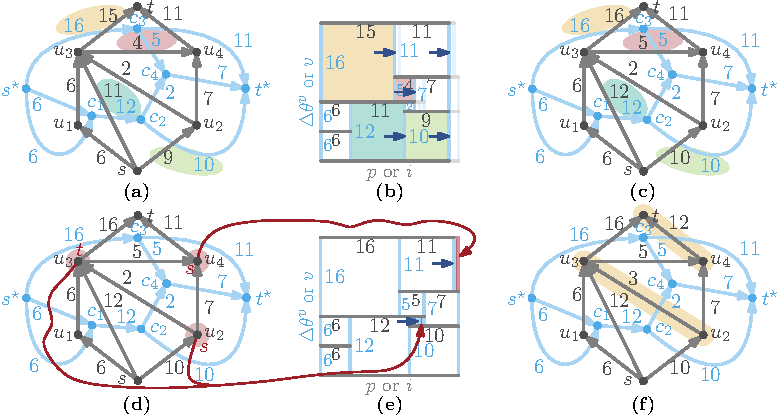
\includegraphics{networkAnalyzes/figures/geometric-interpretation-of-a-kcl-conflict.pdf}
    %
    \caption[KCL Conflict Resolution.]{A \textcolor{PRIMALGRAPH}{primal
    graph~\glssymbol{graph}} and its \textcolor{DUALGRAPH}{dual
    graph~\glssymbol{dualgraph}} that have each six vertices, nine edges, one
    source and one sink are shown in (a), (c), (d), and (f). A geometrical
    representation of both graphs is given in (b) and (e). Each edge in either
    graphs represents a line segment in the appropriate color and the flow on an
    edge defines the aspect ratio of a rectangle, \eg, the
    edges~$\textcolor{DUALGRAPH}{(\cycle_3,\sink^\star)}$ and~$
    \textcolor{PRIMALGRAPH}{(\vertexa_4,\sink)}$ describe
    the~\textcolor{DUALGRAPH}{height} and~\textcolor{PRIMALGRAPH}{width} of the
    upper right rectangle, respectively. (a) A change in flow in the dual graph
    causes a mapping, which effect is shown in (b) and (c). (b) The mapping
    causes a rescaling of some rectangles sides, \ie, in this case the width of
    four rectangles are changed. The outer hull changes from a rectangle to a
    non-rectangle (shown in the background). (c) After the mapping step the
    one-to-one-correspondence is retained. (d) In this case the mapping result
    in a~\gls{kcl} conflict (red) in the primal
    graph~\textcolor{PRIMALGRAPH}{\gls{graph}}. (e) Resizing the two rectangles
    resolves the conflict. (f) The flow on the edges~$(\vertexa_2,\vertexa_3),
    (\vertexa_4,\sink)\in\glssymbol{edges}(\glssymbol{graph})$ resolves the
    conflict. }
    % 
    \label{ch:network-analyzes:sec:algorithm:fig:geometric-interpretation-of-a-kcl-conflict}
\end{figure}
% 
% 
\begin{definition}[Minimal Conflict Resolution]
    % 
    The shortest path~$\glssymbol{path}_{\gls{spp}}$ and the longest
    path~$\glssymbol{path}_{\gls{lpp}}$ are defined by~$
    % 
        \fpath{\gls{spp}}{\source}{\sink}
        \coloneqq
        \argmin_{ \fpath{}{\source}{\sink} \in \glssymbol{pathset} } 
        \sum_{\edge\in\fpath{}{\source}{\sink}}
        \nicefrac{
            \glssymbol{flow}(\edge)
        }{
            \glssymbol{susceptance}(\edge)
        }
    % 
    $ with a length of $
        % 
        \glssymbol{voltageangledifference}(\fpath{\gls{spp}}{\source}{\sink})
        % 
    $ and~$
        % 
        \fpath{\gls{lpp}}{\source}{\sink}
        \coloneqq \argmax_{\fpath{}{\source}{\sink} \in \glssymbol{pathset} } 
        % 
    $ 
    % 
    $
    % 
        \sum_{\edge\in\fpath{}{\source}{\sink}}
        \nicefrac{\glssymbol{flow}(\edge)}{\glssymbol{susceptance}(\edge)}
    % 
    $ with a length of $
        % 
        \glssymbol{voltageangledifference}(\fpath{\gls{lpp}}{\source}{\sink})
        % 
    $, respectively. A conflict resolution in one graph causes a flow change in
    either graphs and thus, the minimum conflict resolution is defined
    in~\glssymbol{graph} and~\glssymbol{dualgraph} by:
    % 
    \begin{compactenum}[\hspace*{1cm}(CR--1)]
    % 
    \item
    Let~$\fpath{\gls{spp}}{\source^\star}{\sink^\star},\fpath{\gls{lpp}}{\source^\star}
    {\sink^\star}\in\glssymbol{pathset}(\glssymbol{dualgraph})$ then a conflict
    resolution in~$\glssymbol{dualgraph}$ is of minimum size if and only
    if~$    
        % 
        \glssymbol{voltageangledifference}(
            \fpath{\gls{spp}}{\source^\star}{\sink^\star}
        ) 
        = 
        \glssymbol{voltageangledifference}(
            \fpath{\gls{lpp}}{\source^\star}{\sink^\star}
        )
        % 
    $.
    % 
    \label{ch:network-analyzes:CR:1}
    % 
    \item
    Let~$
        % 
        \fpath{\gls{lpp}}{\source}{\sink}
        \in
        \glssymbol{pathset}(\glssymbol{graph})
        % 
    $, and
    let~$
        % 
        \glssymbol{voltageangledifference}'(
            \glssymbol{path}_{\gls{lpp}}(\source,\sink)
        )
        % 
    $ and~$
        % 
        \glssymbol{voltageangledifference}(
            \glssymbol{path}_{\gls{lpp}}(\source,\sink))
        % 
    $ be the longest path before and after the change. Then a conflict
    resolution in~$\glssymbol{graph}$ is minimum if and only if the change of
    the longest path~$
    % 
    \Delta_{\gls{lpp}}(\source,\sink)
    \coloneqq
    \glssymbol{voltageangledifference}'(\glssymbol{path}_{\gls{lpp}}(\source,\sink))
    -
    \glssymbol{voltageangledifference}(\glssymbol{path}_{\gls{lpp}}(\source,\sink))
    % 
    $
    is minimized~$
    \min\Delta_{\gls{lpp}}(\source,\sink)
    $.
    % 
    \label{ch:network-analyzes:CR:2}
    % 
    \end{compactenum}
    % 
    We call a conflict resolution minimum if and only
    if~\mbox{CR--\ref{ch:network-analyzes:CR:1}} and
    \mbox{CR--\ref{ch:network-analyzes:CR:2}} holds.
    % 
    \label{ch:network-analyzes:CR}
    % 
\end{definition}
% 
% \begin{proof}
    The conflict resolution~CR--\ref{ch:network-analyzes:CR:1} does not change
    the length of the longest path, but adjusts the length of the shortest path
    to the longest path resulting in a~\gls{kvl} feasible flow. The only
    conflict resolution that changes the length of the longest path
    is~CR--\ref{ch:network-analyzes:CR:2}. However, this represents the smallest
    possible change, since we chose the smallest change of the longest path
    among all choices of changes.% \end{proof}

This can be formulated as an~\gls{lp}, where~CR--\ref{ch:network-analyzes:CR:2}
is an objective and~CR--\ref{ch:network-analyzes:CR:1} is a constraint.
CR--\ref{ch:network-analyzes:CR:1} is illustrated
in~\cref{ch:network-analyzes:sec:algorithm:fig:geometric-interpretation-of-a-kcl-conflict}\screen{d--f},
where the width of the outer rectangle does not change, which is equivalent to
not changing longest path. CR--\ref{ch:network-analyzes:CR:2} is shown
in~\cref{ch:network-analyzes:sec:algorithm:fig:geometric-interpretation-of-a-kcl-conflict}\screen{a--c},
where we solved a conflict in the dual graph~\glssymbol{dualgraph}, which leads
in the mapping step to a change of the width (\ie, change in the longest path of
the primal graph~\glssymbol{graph}).
% 
We now use the aforementioned definition (see~\cref{ch:network-analyzes:CR}) for
a minimum conflict resolution to formulate an algorithm for the conflict
resolution step~\resolveConflict{$\subgraph,
\excessSet, \source, \sink,$ $\glssymbol{flow}_{\subgraph}$}. The set
of~\gls{kcl} conflicts is given by~$
    % 
    \excessSet 
    \coloneqq 
    \{
        \vertexa
        \in
        \glssymbol{vertices}(\subgraph)
        \mid
        \glssymbol{netflow}(\vertexa)
        \neq 
        0
    \}
    % 
$, where~\subgraph is either~\glssymbol{graph} or~\glssymbol{dualgraph}. The
conflict resolution CR--\ref{ch:network-analyzes:CR:1} implies that the edges
for the conflict resolution should lie on
path~$
    % 
    \fpath{ }{\source^\star}{\sink^\star}
    % 
$ with~$
    % 
    \fpath{ }{\source^\star}{\sink^\star} 
    < 
    \fpath{ \gls{lpp} }{\source^\star}{\sink^\star}
    % 
$ of~$
    % 
    \subgraph^{\star} 
    =
    \algoDualGraphOf(\subgraph, \source, \sink)
    % 
$. Thus, a possibility is to compute the shortest path graph
in~$\subgraph^\star$. We save all edges in a set of candidate
edges~$\glssymbol{edges}'$.
% 
% Since the length of~$\fpath{\gls{lpp}}{\source}
% {\sink}$ should not change, but the length of~$\fpath{\gls{spp}}{\source}
% {\sink}$ should be adjusted to the length of the longest path, it suffices to
% select two terminals. 
% 
We define excesses accordingly by~$
    % 
    \source, 
    \vertexa_{\source} 
    \in 
    T_{\source}
    % 
$ and~$
    \sink, 
    \vertexa_{\sink} 
    \in
    T_{\sink}
$.

The conflict resolution~CR--\ref{ch:network-analyzes:CR:2} corresponds to a
minimum change of the longest path in~\subgraph. We have to evenly distribute
the flow excess at each vertex~$
    % 
    \vertexa
    \in
    \excessSet
    \subseteq
    \glssymbol{vertices}
    % 
$ along all paths. Since we wish to minimize~$
    % 
    \Delta_{\gls{lpp}}(\source,\sink)
    \coloneqq
    \glssymbol{voltageangledifference}(\glssymbol{path}_{\gls{lpp}}'(\source,\sink))
    -
    \glssymbol{voltageangledifference}(\glssymbol{path}_{\gls{lpp}}(\source,\sink))
    % 
$, we increase the flow only at edges on the shortest paths~$
    % 
    \fpath{\gls{spp}}{\source'}{\sink'}
    % 
$ in the dual graph until either~$\source'$ or~$\sink'$ are saturated.

We augment iteratively one unit of flow along the shortest~\source-\sink-path
from~$
    % 
    \source' 
    \in 
    T_{\source}\setminus\source
    % 
$ to~$
    % 
    \sink' 
    \in 
    T_{\sink}\setminus\sink
    % 
$ using the metric~$
    % 
    \nicefrac{
        \glssymbol{flow}
    }{
        \glssymbol{susceptance}
    }
    % 
$ until all~$
    % 
    \source'
    \in 
    T_{\source}, 
    \sink'
    \in 
    T_{\sink}
    % 
$ have~$\glssymbol{netflow}(\vertexa) = 0$ with~$
    % 
    \vertexa
    \in
    (
        T_{\source}
        \cup 
        T_{\sink}
    )
    \setminus
    \{\source,\sink\}
    % 
$.
% 
% The sweep line algorithm~$\sweepLineFlowAlgorithm(\vertexa,\glssymbol{netflow}
% (\vertexa),\subgraph', \glssymbol{flow})$
% (see~\cref{ch:network-analyzes:algo:sweepline-algorithm}) is a simple
% modification of a~\gls{bfs} along the shortest path graph from u to t' and
% at each vertex in the BFS we split the flow according to the number of
% outgoing incident edges
% (see~\cref{ch:network-analyzes:algo:sweepline-algorithm}
% in~\cref{ch:network-analyzes:algo:sweepline-algorithm:split}).
% 
% \begin{algorithm}[tb!]%
% \SetAlgoLined
% %%%%%%%%%%%%%%%%%%%%%%%%%%%%%%%%%%
% % 
% \KwData{A directed \source-\sink-graph~$\subgraph$, one source~$\source$, one
% sink~$\sink$, an initial excess~$e'$, and flows~$\glssymbol{flow}
% (\vertexa,\vertexc)$ with~$(\vertexa,\vertexc)\in\glssymbol{edges}$.}%
% \KwResult{Modified flow~$\glssymbol{flow}(\vertexa,\vertexc)$ for all $
% (\vertexa,\vertexc)\in\glssymbol{edges}(\subgraph)$.}
% % 
% % INITIALIZATION %%%%%%%%%%%%%%%%%%%%%%%%%%%%%%%%%%%%%%%%%%%%%%%%%%%%%%%%%%%%
% $\netflow(\vertexa) = e'$\; % vertexa is initial source
% % 
% % LOOP UNTIL QUEUE IS EMPTY %%%%%%%%%%%%%%%%%%%%%%%%%%%%%%%%%%%%%%%%%%%%%%%%%
% \While(\Comment*[f]{\color{KITblack30}Sweep line Resolution of a~\gls{kcl}
% conflict for an~\source-\sink-pair in~\subgraph})% basically a simple BFS search
% % BFS search
% {$\mathcal{Q}\not=\emptyset$}
% { % while
%     $\vertexa = \mathcal{Q}.\deleteFirst()$\;
%     $\flow(\vertexa,\vertexc)
%             = 
%             \flow(\vertexa,\vertexc)
%             + 
%             \frac{\lceil\netflow(\vertexa)\rceil}{\fmagnitude{\outneighbor(\vertexa)}} 
%             \qquad\forall 
%             \vertexc\colon(\vertexa,\vertexc)\in\edges(\subgraph)$\;
%             \label{ch:network-analyzes:algo:sweepline-algorithm:split}
%     % 
%     $\mathcal{Q}.\pushBack(\vertexa)\qquad\forall\vertexa\in\outneighbor
%     (\vertexa)$\;
% }
% 
% %%%%%%%%%%%%%%%%%%%%%%%%%%%%%%%%%%
% \caption{\texttt{sweepLineFlowAlgorithm}}%
% \label{ch:network-analyzes:algo:sweepline-algorithm}%
% \end{algorithm}% 
% 
\begin{conjecture}
    \Cref{ch:network-analyzes:algo:s-t-power-flow-algorithm} computes a
    correct \source-\sink electrical flow of minimum integral size.
    % 
    \label{ch:network-analyzes:lem:minimum-integer-flow}%
\end{conjecture}
% 
% \begin{proof}
We give an idea how we think the proof could work.
% 
    Let~$\glssymbol{flow}(\edge)$ be a minimal integral electrical flow. Let~$
    \glssymbol{flow}'(\edge)$ be some flow with~$ %
        \glssymbol{flow}'(\edge) 
        \leq 
        \glssymbol{flow}(\edge)
        % 
    $ for all~$\edge\in\glssymbol{edges}$ and the flow~$\glssymbol{flow}'$
    fulfills the~\gls{kvl}. We claim that there is a~$
        % 
        \glssymbol{flow}''(\edge)
        =
        \glssymbol{flow}(\edge)
        % 
    $ for all~$\edge\in\glssymbol{edges}$. Assume that there is an edge~$
        % 
        \glssymbol{flow}''(\vertexa,\sink) 
        = 
        \glssymbol{flow}'(\vertexa,\sink) 
        + 1
        >
        \glssymbol{flow}(\vertexa,\sink) 
        % 
    $ meaning the flow would skip a minimal integral solution. This would mean
    that there is another path from~\vertexa to~\sink with~$
    \glssymbol{flow}'''$. Since~$
        % \glssymbol{flow}'(\vertexa,\sink) 
        % = 
        \min_{\fpath{}{\vertexa}{\sink}\in\glssymbol{pathset} } 
        \sum_{(\vertexa,\vertexb)\in\fpath{}{\vertexa}{\sink}}
        \frac{ 
            \glssymbol{flow}(\vertexa,\vertexb) 
        }{ 
            \glssymbol{susceptance}(\vertexa,\vertexb) 
        }
        =
        \min_{\fpath{}{\vertexa}{\sink}\in\glssymbol{pathset} } 
        \sum_{(\vertexa,\vertexb)\in\fpath{}{\vertexa}{\sink}}
        \glssymbol{voltageangledifference}(\vertexa,\sink)
    $ this represents a contradiction.

    % We proof the correctness of the lemma by induction. 
    % 
    We assume that the conjecture is correct for any \source-\sink plane
    graph~\glssymbol{graph} as long as~\glssymbol{graph} constitutes an
    electrical flow. Assuming a graph with~$
    \fmagnitude{\glssymbol{undirectededges}} = 1$ then applying a flow
    of~$\glssymbol{flow}(\source,\sink) = 1$ along an edge incident to~\source
    (which is here the only edge~$ (\source,\sink)$) results in a feasible
    flow~$\glssymbol{flow}_{\glssymbol{graph}}$ in~$\glssymbol{graph}$ and in a
    feasible flow~$\glssymbol{flow}_{\glssymbol{dualgraph}}$
    in~$\glssymbol{dualgraph}$ accordingly.

    Now, we assume an arbitrary \source-\sink plane graph~\glssymbol{graph}. The
    construction of the graph is correct
    (see~\cref{ch:network-analyzes:sec:planar-embedding-dual-graph-construction}).
    Since we resolve each conflict optimal meaning using the minimum number of
    changes in each conflict resolution (see~\cref{ch:network-analyzes:CR}) and
    we push only flow in the predefined direction, we get an order of increasing
    flows and using the minimum conflict resolution does not skip a solution.
    Since we know that
    \glssymbol{graph} has an electrical flow the algorithm terminates.
    % 
    % \franzi{This whole thing reminds me on Benders decomposition, structure is
    % very similar. (Maybe) establish connection to it. }
    % 
    % 
% \end{proof}
% 
% The algorithm terminates in polynomial time, since~\gls{dc}~\gls{feas}
% constitutes a rational polytope this is proven
% in~\cref{ch:network-analyzes:sec:mathematical-model:lem:integral-e-flow-poly-size}.
% 

% 
% Superposition and scaling gives us an electrical flow for multiple sources and
% sinks.
% 
% For Max power flow maybe dynamic programming.
% 
% \begin{figure}
%     % 
%     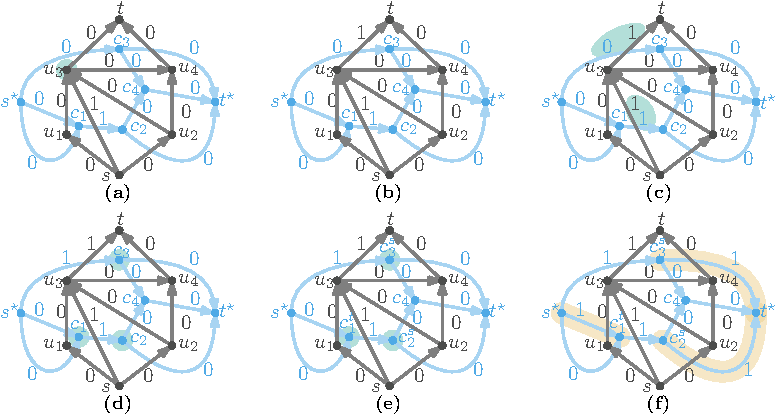
\includegraphics{networkAnalyzes/figures/AlgorithmicSteps.pdf}
%     % 
%     \caption[Example that shows the main steps of the algorithm.]{An example
%     showing the main steps of the algorithm to compute a
%     electrical flow~\glssymbol{flow} on a graph~\glssymbol{graph}. Note that
%     this is the exact same example provided by~\textcite[p.18]{Fel13}. (a)
%     Augmenting~$1$ unit along the shortest path from~\source to~\sink. (b)
%     Mapping step with~$\glssymbol{flow}_{\glssymbol{dualgraph}}(\edge) =
%     \glssymbol{flow}_{\glssymbol{graph}} (\oneToOneMap(\edge))$ for
%     all~$\edge\in\glssymbol{edges}$. (c) \gls{kcl} conflict
%     meaning~$\glssymbol{netflow}(\vertexa)\neq 0$ for
%     some~$\vertexa\in\glssymbol{vertices}$. (d) Define temporary sources and
%     sinks. (e) Compute flow from~$\glssymbol{generators}\coloneqq
%     \{\source,\vertexa_{\source},\vertexb_{\source}\}$
%     to~$\glssymbol{consumers}\coloneqq\{\vertexc_ {\sink},\sink\}$, where
%     temporary terminals have fixed demand and supply. (f) Resulting electrical
%     flow~\glssymbol{flow}.
%     % 
%     }
%     % 
%     \label{ch:network-analyzes:sec:mathematical-model:fig:algorithm}%
% \end{figure}
% 
%%%%%%%%%%%%%%%%%%%%%%%%%%%%%%%%%%%%%%%%%%%%%%%%%%%%%%%%%%%%%%%%%%%%%%%%%%%%%%%%
\section{Conclusion}
% \label{}
%%%%%%%%%%%%%%%%%%%%%%%%%%%%%%%%%%%%%%%%%%%%%%%%%%%%%%%%%%%%%%%%%%%%%%%%%%%%%%%%
% 
This chapter provides a thorough analysis of electrical flows. In the beginning,
we showed different properties of electrical flows as well as methods that are
essential in the first place to design an electrical flow algorithm for planar
graphs and matroids. We give a first algorithm for~\source-\sink electrical
flows that uses electrical preserving transformations and has a running time
of~$
    % 
    \bigO(\fmagnitude{\glssymbol{vertices}}^3)
    % 
$. This is better than the known exponential time algorithm mentioned
in~\cref{ch:network-analyzes:sec:mathematical-model:lem:current_edge_from_a_to_b}.
Even though both algorithms are constructive and exploit some structure, there
is a comparable computation of electrical flows that needs polynomial time for
arbitrary networks. To give electrical flows more structure, we present
different graph-theoretic representations. These representations help us to
separate the quadratic relationship and lead to the balancing property, which
will be used in an algorithmic approach that computes~\source-\sink electrical
flows by using two graphs that are dual
(see~\cref{ch:network-analyzes:sec:algorithm}).

There are still some open conjectures and research questions that we would like
to investigate. One of the first questions, we try to investigate is the running
time and correctness of~\cref{ch:network-analyzes:algo:s-t-power-flow-algorithm}
that depends on the unknown minimum integral generation and demand vector. For
arbitrary susceptances~\glssymbol{susceptance} the resolution can have
exponential size. However, if we restrict the resolution to some ratio, we might
be able to restrict the vector and the running time.

Recall that one assumption on our graphs is that they are planar. On general
graphs that cannot be embedded planar on a plane surface (\ie, surface with
genus 0), we do not have the concept of faces. However, if we chose a surface
with higher genus that allows a plane embedding of the graph, we can make use of
the aforementioned algorithms. Thus, we raise the following conjecture.
% 
\begin{conjecture}
    % 
    \footnote{We thank Peter Sanders for the discussion on that topic. In
    addition, we like to thank Thomas William Brown for mentioning and
    describing Cohomology to us.}
    % 
    \Cref{ch:network-analyzes:algo:s-t-power-flow-algorithm} or the algorithm
    from~\cref{ch:network-analyzes:sec:mathematical-model:thm:algo-pf-1}
    are~\gls{fpt} in the genus.
    % 
\end{conjecture}
% 
We note that computing all~\source-\sink electrical flows, adding them, and
scaling them leads to a multi-source multi-sink electrical flow algorithm that
is not very efficient. Though it might be in general inefficient, it is worth
investing these algorithms for dynamic power grids that make use of the
\source-\sink-decompositions while starting with some initial electrical flow.
%